\chapter{Origins of Multi-decadal Variability in Sudden Stratospheric Warming events}
\label{cha:models}
\begin{quotation}
  Much of the work presented in this chapter is based on \cite{dimdore-milesOrigins2020b} however the analysis has been extended here to include a more comprehensive diagnosis of stratospheric variability in the.
\end{quotation}


\section{Introduction}
\label{sec:origins_introduction}
Despite a significant body of work aimed at understanding the nature of vortex variability including SSWs, variations in this mode on decadal to multi-decadal timescales is not well understood. A formal diagnosis of such variability as well as a better understanding of factors which influence it may help to improve predictability of SSWs and subsequently NH mid-latitude surface climate \cite{.

There is some evidence of vortex variations with periods longer than a year in the observational record. In reanalysis datasets, SSWs occur at an average rate of $\sim$0.6 events/winter but this varies markedly within the record \citep{butlerDefining2015b} suggesting the possibility of variability on much longer timescales. For example, observational studies have noted a hiatus in the 1990s when very few major SSW events occurred \citep{butlerDefining2015b,pawsonCold1999b, Shindell1999} while, in contrast, the early 21st century displayed a remarkable number of consecutive winters containing SSW events \citep{manneyRemarkable2005}. Other studies have addressed the notion of low frequency variations in the vortex using GCMs. \cite{garfinkelStratospheric2017b} analyse decadal-scale variations in vortex strength in a set of historical simulations and propose that an observed hiatus in Eurasian surface warming was most likely due to variability in midwinter vortex strength. Similarly, \cite{cohenDecadal2009b} find decadal scale variations in planetary wave forcing of the vortex in a suite of CMIP3 models as well as NCEP–NCAR reanalysis. Whether the vortex variability was forced by greenhouse gas concentrations or arose through internal variability in these studies was not fully established but \cite{garfinkelEffect2015b} used a subset of the simulations analysed in \cite{garfinkelStratospheric2017b} and linked a decadal trend (1980-2009) in late winter vortex strength to SST variability. On the other hand, \cite{Seviour2017} analysed observed variations between 1980 and 2016 and concluded that the vortex variability was primarily internally generated. Other studies also point towards internally generated decadal fluctuations in vortex strength: \cite{manziniStratospheretroposphere2012b} explore causes of 20 year period variability in a simulation with prescribed, pre-industrial SSTs. They propose that, given the boundary conditions in the simulations are fixed, such variability must be internally generated. Finally, \cite{Butchart2000} suggest that decadal variability in vortex strength as well as SSW frequency may originate from feedbacks caused by the non linear nature of boreal winter stratospheric dynamics.

On longer timescales, \cite{schimankeMultidecadal2011b} note variations in SSW occurrence with periods of approximately 52 years in a multi-century GCM integration and demonstrated coherent variability in other parts of the climate system, including vertically propagating planetary wave activity, Eurasian snow cover and Atlantic SSTs. However, despite providing some indications of externally driven variability, results from this study are not conclusive, since the GCM used (EGMAM: ECHO‐G with Middle Atmosphere Model) exhibits significant bias in mean SSW rate compared to reanalyses (2 events per decade compare to $\sim$6 in reanalysis). The authors also note that further simulations are required to understand this variability. 

multi-decadal scale variations in climate features which can couple with the vortex has also been explored. There are clear decadal variations in the period and phase transition timing of the QBO \citep{pascoeQuasibiennial2005b,ansteyResponse2008b,Yang2016}. These may be linked to variations in the degree of 'stalling' of the QBO phase descent, which can cause more or less persistent wind direction at a given level.  A number of studies have also noted the transient nature of the strength of the HT relationship \citep{luDecadalscale2008,luMechanisms2014c,ansteyResponse2008b,ospreyClimatology2010b}. \cite{luDecadalscale2008,luMechanisms2014c} show that the mid-latitude wave-guide is modulated by the shape of the vortex so that planetary waves are diverted further equatorwards when the vortex is anomalously strong and wide, and this could temporarily reduce the influence of the QBO on the vortex. The Aleutian Low (see section \ref{sec:external_influence_AL}) also varies significantly on decadal to multi-decadal timescales. \cite{overlandDecadal1999b} note that 10 year mean values of SLP over the AL region exhibit fluctuations of up to 35\% of the climatological mean. Subsequent studies corroborate the presence of these decadal scale fluctuations: \cite{SUGIMOTO2009} and \cite{Minobe} show 20 year fluctuations in intensity and centre of action of the AL while \cite{Raible2005} propose a 50-60 year trend in AL intensity, suggesting the existence of even longer timescale variability. 

Although substantial effort has been applied to characterising SSWs and their underlying mechanisms, there is little understanding of periods of hiatus (such as that in the 1990s) and consecutive-event years (early-mid 2000s), primarily because of the short record of reliable observations as well as the complexities and often non-stationary nature of the multiple observed teleconnections. Much longer time-series are required to successfully identify and understand the source of decadal and multi-decadal scale variability. In the meantime, analysis of variability and teleconnections in long climate model simulations may help to understand these processes. 

In this chapter, we analyse long-term variability of the stratospheric polar vortex in a 1000-yr pre-industrial (pi-cntrl) simulation of the UK Earth System Model (UKESM). The absence of external forcings such as greenhouse gas increases, volcanic and solar variations allows us to examine sources of long-term variability that are internally generated within the climate system. We identify intervals containing high and low SSW rates and analyse their variability, with a focus on multi-decadal scales. A variety of techniques are employed to examine associations with those parts of the climate system that are known to exhibit long-term memory, namely the tropical SSTs and the related Aleutian Low. In particular, a wavelet spectral decomposition and cross-spectrum analysis is employed to overcome some of the difficulties with non stationary signals that may arise. We also investigate interactions between the polar vortex and the QBO as a potential source of internally-driven variability.

\section{Data And Methods}

\subsection{Model Configuration}
\label{sec:model_config}
For analysis of multi-decadal variability in the vortex and SSWs, we utilise a simulation of the first version of the UK Earth System Model (henceforth referred to as UKESM), a configuration of the MetOffice unified model (the UM) \citep{mulcahyImproved2018b}. UKESM is a stratosphere resolving coupled ocean-atmosphere-land-sea ice model. The Atmospheric component is GA7.1 with 85 vertical levels from the surface to 85km, 35 of which are above 18km \citep{waltersMet2019b, williamsMet2018b}. The model is run at N96 horizontal resolution (approximately 135 km near the equator). The ocean model used is GO6.0 \citep{Storkey2018} which contains 75 levels and runs at 1${^\circ}$ horizontal resolution. Land surface and sea-ice processes are represented by JULES \citep[GL7.0,][]{waltersMet2019b} and CICE  \cite[GSI8.1,][]{ridleySea2018b} models respectively, while ocean biochemistry is added through MEDUSA \citep{Yool2013}. UKESM also includes a fully interactive chemistry scheme via coupling with the UK Chemistry and Aerosols model \citep[UKCA,][]{mulcahyImproved2018b}.

We utilise a 1000 year pre-industrial (PI) control simulation of UKESM submitted to CMIP6 which is spun-up to achieve initial model equilibrium following the method outlined in \cite{yoolSpinup2020b}. This run is forced using CMIP6 pre-industrial values for concentrations of major GHGs (global mean 284.317ppm $CO_2$, 808.25ppb $CH_4$, 273.02ppb $N_2O$). While there are no volcanic eruptions in the simulation, background stratospheric volcanic aerosols are set to climatological values between 1850 and 2014 estimated from satellite products and other model simulations \citep{menaryPreindustrial2018b}. We choose a PI control for this analysis to examine internal variability in SSWs on multi-decadal timescales. 

\subsection{Reanalysis Data}
\label{sec:ERA_data}
To verify that the model reproduces relevant features of the climate system we compare with an observation based dataset produced by the ECMWF - ERA-Interim \cite{Dee2011}. The ERA-interim dataset is produced by a 4D-Var data assimilation method of a wide range of observations \citep{Uppala2005}. These include surface measurements, aircraft campaign data, radiosonde readings and satellite observations. The 4D-var data assimilation process involves supplying the ECMWF’s Integrated Forecast System (IFS) initial conditions from observations, letting the model evolve for a timestep and re-initialising for the next step with a combination of output and updated observations \citep{courtierECMWF1998, bouttierObservingsystem2001a}. This update is carried out to minimise a cost function defined to capture the difference between the latest model output and observations for that corresponding time. ERA-Interim provides data on 60 vertical levels at a maximum horizontal resolution of $\sim$ 80 km from 1979-2019 \citep{Berrisford}.

The majority of observations assimilated for ERA-Interim are satellite based radiance retrievals. These are gained from nadir facing satellites which measure spectral radiances (energy detected at difference wavelengths). A single detection device will consist of several channels which detect radiation from difference wavelengths. Different atmospheric layers absorb and emit at different wavelengths so measuring over a range of channels can build up a vertical profile of a variable such as temperature. However, the atmospheric layers that are detected by each channel may overlap resulting in measurements from multiple channels being used in the retrieval of a given layer. A weighting is applied to the channels at each height to account for the proportion of the total measurement that should be contributed by each channel. Channel weighting profiles (see figure \ref{fig:Satellite_channels}) are generally Gaussian (for Nadir Satellites) in pressure coordinates \citep{fujiwaraIntroduction2017}, the width of which signifying the vertical extent of the channel. The vertical resolution of the retrievals is determined by the density of channels covering a particular height range. 

During the ERA-Interim period, the set of observations used for assimilation have developed significantly. Between 1979 and 1998 only limited satellite based radiance retrievals are available to produce profiles. These satellite observations are primarily provided by the Stratosphere Sounding Unit (SSU) and Microwave Sounding Unit (MSU) which are parts of the TRIOS Operational Vertical Sounder (TOVS) suite. The SSU possesses only 3 channels (figure \ref{fig:Satellite_channels}a) and therefore provides data at relatively coarse vertical resolution. Over this period, ERA-interim relies heavily on direct measurement techniques such as radiosondes, dropsondes and aircraft \citep{fujiwaraIntroduction2017} which bring possible biases from the influence of shortwave solar heating on temperature sensors in radiosondes as well as warmer tendencies in aircraft based observations compared to radiosondes \citep{ballishSystematic2008}. After 1998 more extensive satellite based measurements are available for assimilation and are incorporated in ERA-interim. The new satellite products include improved versions of the SSU and MSU as a part of the Advanced TRIOS Operational Vertical Sounder (ATOVS) suite which provides profiles derived from the Advanced Microwave Sounding Unit A (AMSU, figure \ref{fig:Satellite_channels}b) from which ERA-interim calculates profiles using 11 channels (channels 5-14 from AMSU). ERA-Interim also makes use of a number of other satellite based instruments which are fully outlined in \citep{fujiwaraIntroduction2017}. Possible sources of biases in these satellite based observations include orbital drift and calibration offsets \citep{simmonsEstimating2014}.

As a result of including additional observations for assimilation after 1998, ERA-interim shows a shift in temperature structure of the middle and upper stratosphere between the two periods. Caution is therefore advised when using this data for trend analysis \citep{longClimatology2017} however such an analysis does not form part of the work in this thesis. Zonal wind fields show little change across the periods. Additionally, ERA-interim struggles (as the majority of modern reanalyses do) to constrain phase transition timing of the QBO correctly \citep{kawataniRepresentation2016}. Comparisons with wind profiles derived from a single radiosonde station (Singapore at $^{\circ}$1N, $104^{\circ}$E), which covers a large majority of the reanalysis period, show that ERA-interim also exhibits biases in the amplitude of both QBO phases. These biases reduce significantly with the transition to the use of ATOVS \citep{kawataniRepresentation2016,longClimatology2017}. Similar biases and improvements over the TOVS-ATOVS period are also observed for representation of the SAO \cite{baldwinTropical2005}. These biases must be taken into account when considering comparisons in stratospheric circulation between ERA-interim and GCMs. Nonetheless, \cite{longClimatology2017} stress that these datasets are in broad agreement with other major reanalyses in the stratosphere and lower mesosphere.

\begin{figure}[h!]
\centering
    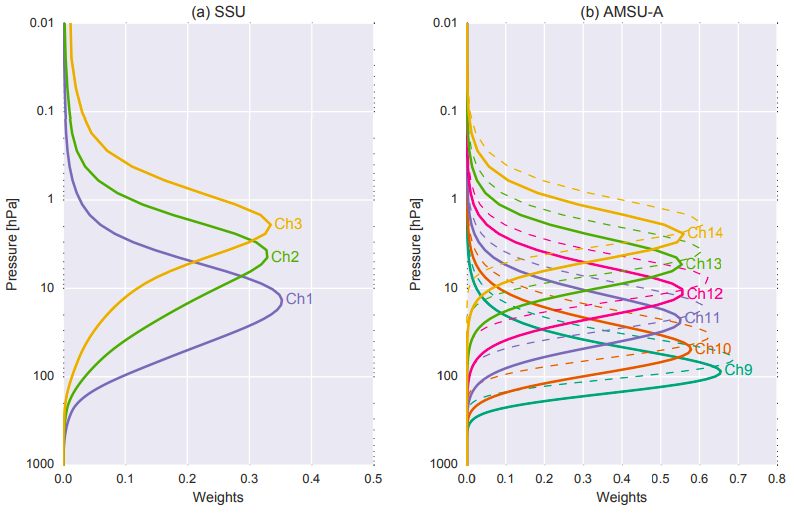
\includegraphics[width=0.85\textwidth]{Figures/Figures-origins/channels.png}
    \caption[Channel profiles for satellite retrievals assimilated by ERA-Interim]{Figure from \cite{fujiwaraIntroduction2017} \textbf{Left}: Channel weighting profiles for the TOVS Stratospheric Sounding Unit (SSU) used for ERA-Interim dataset in the period 1979-2005. \textbf{Right}: Weighting profiles from the ATOVS-suite Advanced Microwave Sounding Unit (AMSU) which provides measurements for ERA-Interim from 1998-present. Solid lines represent near Nadir profiles and dashed lines signify limb profiles (taken at an angle of $48.33^{\circ}$).}
    \label{fig:Satellite_channels}
\centering
\end{figure}

\subsection{Wavelet Analysis}
\label{sec:Wavelet_Analysis}
In order to study possible multi-decadal variability in SSW occurrence, we utilise a wavelet analysis method based on \cite{Torrence1998}. Such an analysis can be used to examine time series which displays non-stationary spectral power over multiple frequencies \citep{Daubechies} giving it a useful advantage over more traditional fourier methods for spectral analysis. The wavelet transform of a uniform 1-dimensional time series, $x$, of length $N$ and timestep $\delta t$ is given by the convolution between the series and a scaled and translated version of a wavelet function $\psi_0$ (equation \ref{wavelet_transform})

\begin{equation} \label{wavelet_transform}
W_n(s) = \sum^{N - 1}_{n' = 0} x_{n'} \psi^* \bigg[(n' - n) \frac{\delta t}{s}\bigg],
\end{equation}

where $*$ denotes the complex conjugate and $s$ is the wavelet scale indicating the frequency of the wavelet. Varying $s$ and translating along the time scale (the index $n$), $W_n$ indicates the amplitude of signals at different scales and their variation in time. \cite{Torrence1998} suggest an approach to varying the scale s as increasing in powers of 2 according to 

\begin{equation} \label{S}
s_j = s_0 2^{j \delta j},\\ j = 0, 1, ..., J
\end{equation}

\begin{equation} \label{S}
J = \delta j^{-1} log_2\bigg(\frac{N \delta t}{s_0}\bigg),
\end{equation}

where $s_0$ is the shortest resolvable scale of a signal, J corresponds to the longest and $\delta j$ is the scale resolution. The translated and scaled wavelet has the form

\begin{equation} \label{wavelet}
\psi^* \bigg[(n' - n) \frac{\delta t}{s}\bigg] = \bigg(\frac{\delta t}{s}\bigg)^{1/2} \psi_0\bigg[(n' - n) \frac{\delta t}{s}\bigg]
\end{equation}

and we select the form of $\psi_0$ following the recommendation of \cite{Torrence1998} as a Morlet wavelet, an oscillatory function enveloped by a Gaussian which is expressed as

\begin{equation} \label{psi0}
\psi_0(p) = \pi^{-1/4} e^{i\omega_0 p} e^{\frac{p^2}{2}}.
\end{equation}

The advantages of using a Morlet wavelet for analysing signals in climate time-series is discussed in \cite{lauClimate1995b} in which the authors acknowledge that, while truly physical signals should be detected regardless of which wavelet basis is chosen, for best results one should adopt a wavelet function reminiscent of the real signal. They show that when a Morlet wavelet form is utilised, spectral decomposition methods can detect common forms of behaviour exhibited in the variability of time series associated with the Earth's climate. These include time variations in period and amplitude of signals, abrupt changes in periodicity (sudden regime shift to different spectral behaviour) and some forms of rapid changes in series over time. These forms of behaviour are most likely relevant for our analysis of SSWs, therefore we proceed with a wavelet of this form. 

It is computationally quicker to compute the wavelet transform in discrete Fourier space. By the convolution theorem, the transform reduces to multiplication

\begin{equation} \label{wavelet_transform2}
W_n(s) = \sum^{N - 1}_{k = 0} \hat{x}_{k} \hat{\psi}^* (s\omega_k) e^{i \omega_k n \delta t},
\end{equation}

where $\hat{x}_{k}$ and $\hat{\psi}$ are the discrete Fourier transforms of the time series $x$ (equation \ref{fourier1}) and the wavelet function (equation \ref{fourier2}) respectively. These quantities are given by 

\begin{equation} \label{fourier1}
\hat{x}_k = \frac{1}{N} \sum^{N-1}_{n = 0} x_n e^{\frac{-2\pi i k n}{N}}
\end{equation}

\begin{equation} \label{fourier2}
\hat{\psi}(s\omega_k) = \bigg(\frac{2 \pi s}{\delta t}\bigg) \pi^{-1/4}H(\omega_k) e^{-(s\omega_k - \omega_0)^2/2}
\end{equation}

where $H(\omega_k)$ is the Heavyside function and $\hat{\psi}$ is normalised to have unit energy when integrated over all $\omega$. The square modulus of the wavelet transform gives the wavelet power spectrum which indicates relative strength of signals in the time series as a function of signal period and discretised time. In order to directly compare spectra of different indices we normalise all timeseries by subtracting the mean and dividing by its standard deviation before performing the wavelet transform. In order to effectively compare spectral power across a range of frequencies we additionally scale the power spectrum by dividing by the scale parameter ($s_j$ defined above) associated with each frequency. This is done following the methodology of \cite{liuRectification2007} which shows that un-scaled spectra exhibit a bias towards overestimated powers at longer periods and that an effective comparison across timescales is possible with such scaling. We also define a confidence interval for wavelet power observed at a given period and time for a series by assuming a mean background spectrum corresponding to that of a first order autoregressive (AR1, red noise) process modelled by

\begin{equation} \label{rednoise}
x_n = \alpha x_{n - 1} + z_n,
\end{equation}

where $\alpha$ is the lag-1 autocorrelation of the time series and $z_n$ is Gaussian white noise. \cite{Torrence1998} show that such a process's wavelet power spectrum is $\chi^2$ distributed and therefore can be used to define a 95\% confidence interval for any observed power. 

\subsection{Cross Wavelet Spectra}
The cross wavelet spectrum of two time series $x$ and $y$ with associated wavelet spectra $W^x_n$ and $W^y_n$ gives a measure of coincident power (the same period at the same timepoints) between the series. It is given by

\begin{equation} \label{wavelet_cross}
\vert W^{xy}_n(s)\vert = \vert W^{x*}_n(s) W^{y}_n(s)\vert,
\end{equation}

where $W^{x*}_n(s)$ is the complex conjugate of the wavelet power spectrum of $x$ \citep{grinstedApplication2004b}. The complex argument of $W^{xy}_n(s)$ gives the local phase difference between signals in $x$ and $y$ in frequency-time space. The phase relationship between the two time-series can be represented by a
vector that subtends an angle representing the phase difference: On all plots of cross spectra, arrows to the right (left) denoted signals which are in-phase and correlated (anti-correlated). Vertical arrows indicate a phase relationship of $\frac{\pi}{2}$ between the time-series, so that the evolution of
one is correlated with the rate-of-change of the other. As for individual power spectra, we define a confidence interval for which cross power of a larger amplitude is deemed significant (>95\% confidence interval) by comparing power exhibited by actual series with a theoretical red noise process. The cross power of two such AR1 processes is theoretically distributed such that the probability of obtaining cross power greater than a set of red-noise processes is

\begin{equation} \label{wavelet_cross_dist}
D\bigg(\frac{\vert W^{xy}_n(s)\vert}{\sigma_x \sigma_y} < p\bigg) = \frac{Z_\nu(p)}{\nu} \sqrt{P^x_k P^y_k},
\end{equation}

where $\sigma$ denotes the standard deviation of the time series, Z is the confidence interval defined by $p$ ($Z$ = 3.999 for 95\% confidence), $\nu$ is the degrees of freedom for a real wavelet spectrum ($\nu$ = 2) and $P^x_k$ is the theoretical Fourier spectrum of the AR1 process. For a given wavenumber k, this can be expressed as

\begin{equation} \label{theoretical_fourier}
P_k = \frac{1 - \alpha^2}{\vert 1 - \alpha e^{2i\pi k} \vert^2}.
\end{equation}

\subsection{Hilbert Transform}
We utilise a signal processing method known as a Hilbert transform to calculate the instantaneous phasor amplitude of a QBO time series. The Hilbert transform of a time series $x(t)$ can be expressed as

\begin{equation} \label{eq:hilbert1}
\tilde{x} = Hil[x(t)] = \frac{1}{\pi t} * x(t),
\end{equation}

where $\tilde{}$ denotes the transformed series, * signifies a convolution and $t$ is discretised time. Conversely, the original time series can be recovered using an inverse transform expressed as

\begin{equation} \label{eq:hilbert2}
{x(t)} = Hil^{-1}[\tilde{x}(t)] = -\frac{1}{\pi t} * \tilde{x}(t).
\end{equation}

A complex signal which consists of $x(t)$ and its transform is known as the analytic signal of $x$ and can be used to calculate an instantaneous phasor amplitude, $A(t)$, of the signal. $X(t)$ can be expressed as

\begin{equation} \label{eq:hilbert3}
X(t) = x(t) + \tilde{x}(t) i = A(t) e^{i\theta},
\end{equation}

where $A(t)$ is the instantaneous amplitude of the signal and $\theta(t)$ is the instantaneous phase angle - a measure of signal progression through a cycle at time $t$.

\subsection{Statistical Methods}
\label{sec:stat_methods}

\subsubsection*{Student's t-test}
Much of the analysis presented in this chapter, and indeed in the whole thesis, involves comparisons of composite and mean quantities. A two-tailed student's t-test is implemented to test the null hypothesis that two sampled quantities, $x_1$ and $x_2$, with means $\overline{x}_1$ and $\overline{x}_2$ and standard deviations $\sigma_{1}$ and $\sigma_{2}$ are drawn from the same underlying normal distribution. A $t$ statistic is defined by $t = \frac{\overline{x}_1 - \overline{x}_2}{\sigma_{12} \sqrt{\frac{1}{n_1} + \frac{1}{n_2}}}$ where $n_i$ is the number of samples for quantity $i$ and $\sigma_{12}$ is the pooled variance for the two quantities given by $\sigma_{12} = \sqrt{\frac{\sigma^2_2 (n_2-1) + \sigma^2_1(n_1 - 1)}{n_1+n_2-2}}$. Significance on the difference in means can then be estimated by comparing the value of $t$ with a Student's t-distribution to give an associated $p$ value. Differences which give a $p$ value greater than a deemed level (normally 95\%) are deemed significant in which case the null hypothesis of identical means is rejected to this level.

\subsubsection*{Linear Regression Analysis}
We employ a multi-linear regression technique to give an estimate of the relative contributions to SSW variability from the QBO, ENSO and the AL following the method outlined in \cite{Krzywinski}. We model an SSW timeseries of length $n$ which we denote $y$ as 

\begin{equation} \label{regression}
\hat{y} = \beta_0 + \beta_{1}QBO + \beta_{2}ENSO + \beta_{3}AL
\end{equation}

where $\beta_j$ denotes the coefficient of the corresponding index and $\hat{y}$ is the prediction of $y$. We calculate the best estimate for each $\beta$ using an ordinary least square (OLS) estimator which minimises the sum of squared error (SSE) between the predicted $\hat{y}$ and the real time series $y$ with respect to each coefficient. the SSE is given by $SSE = \sum_i^n{(\hat{y}_i - y_i)^2}$.

We can compare the estimated magnitude of the coefficient for each index to analyse the respective contributions to SSW variability. We can also calculate standard error ranges for $\beta$ estimates. The standard error on an estimated value of a true $\beta_j$ (denoted by $\hat{\beta_j}$) is given by 

\begin{equation} \label{regression}
se(\hat{\beta_j}) = \sqrt{\frac{SSR}{n - k} (X^TX)^{-1}_{jj}}
\end{equation}

where SSR is the sum of squared residuals which measures the sum of squared deviations of predicted values from the mean $y$ value, $\overline{y}$. This is given by $SSR = \sum_i^n{(\hat{y}_i - \overline{y})^2}$). $k$ is the number of predictors used in the linear model (in this case 3) and $X$ is an $n \times k$ matrix consisting of the predictor indices. We also define significance levels for $\hat{\beta_j}$ using a one-tailed $t$ statistic (similar to above) with $n-k$ degrees of freedom to test the null hypothesis that $\hat{\beta_j}$ = 0. The $t$ statistic is given by $t = \frac{\hat{\beta_j}}{se(\hat{\beta_j})}$.

\subsubsection*{EOF Analysis}
\label{sec:eof_analysis}
We also utilise a method for diagnosing patterns of variability in a quantity defined on a spatial and temporal grid. Such a method, known as Empirical Orthogonal Function (EOF) analysis decomposes a function, $y$, into a set of basis functions which indicate the spatial patterns that maximises variance in $y$. 

if $y$ is defined on $N$ time points and $M$ spatial points then the time anomalies of $y$, defined as $y' = y - \overline{y}$ ($\overline{y}$ = the time mean of $y$ at each spatial point) can be expressed as an $N \times M$ matrix denoted as $Y$. The EOFs, $e_n$, are subsequently defined as the eigenvectors of the covariance matrix of $Y$, $C = \frac{1}{N-1}Y^TY$, such that $C e_n = \lambda_n e_n$. $\lambda_n$ is the eigenvalue which can be used to give an indication of the proportion of total variance in $y$ explained by the EOF $e_n$. Such a metric, the variance fraction, is given as $v_n = \frac{\lambda_n}{\Sigma_i \lambda_i}$ - the ratio of a given eigenvalue to the sum of all eigenvalues. EOFs are ordered by eigenvalue size such that EOF1 explains the largest fraction of the total variance. Projecting the matrix $Y$ back onto a given EOF, $e_n$, gives the $n^{th}$ Principle Component (PC) timeseries given by $PC_n = Y e_n$. For the majority applications of EOF analysis for diagnosing climate variability, the first 2 EOF patterns sufficiently explains the variance in quantities such as mean sea level pressure (MSLP) or geopotential height. In the work presented here, we utilise EOF and PC analysis to construct climate variability indices such as the NAM, NAO and AL.  

\subsubsection*{SSW Statistics}
In order to assess model representation of vortex variability, we introduce a statistical framework which uses parametric and bootstrapping methods to asses significance levels for differences in SSW abundance across datasets. First, a parametric approach which assumes that the occurrence of any number of SSWs (denoted as $N$) in a given number of winters (denoted by $k$) can be modeled as a Poisson process and is distributed as 

\begin{equation} \label{Poisson}
P(N(k) = n) = \frac{(\lambda k)^n}{n!} e^{-\lambda k},
\end{equation}

where $\lambda$ is the intensity of the Poisson process calculated as the mean SSW rate over $k$ winters. For two such processes with intensities $\lambda_1$ and $\lambda_2$ the difference in intensity, $\Delta\lambda$ can be expressed as

\begin{equation} \label{Poisson}
\Delta\lambda = \frac{\lambda_1 - \lambda_2}{\sqrt{\frac{\lambda_1}{k_1} + \frac{\lambda2}{k_2}}},
\end{equation}

where $k_i$ is the number of instances of process $i$ (number of winters sampled). \cite{Charlton2007} suggest that if a pair of Poisson processes are recorded for more than 30 instances each then $\Delta\lambda$ can be assumed to be normally distributed. \cite{guTesting2008} and \cite{huffmanImproved1984} present an alternative test for the significance of $\Delta\lambda$ in cases where the datasets underlying each process are of different lengths (i.e. for comparing model and reanalysis data). For this analysis, we introduce the test statistic

\begin{equation} \label{deltalambda}
W(X_1, X_2) = 2 \frac{\sqrt{X_1 + 3/8} - \sqrt{\rho(X_2 - 3/8)}}
{\sqrt{1 + \rho}},
\end{equation}

where $\rho$ is the ratio of observation lengths of the datasets and $X_i$ is the number of observations of events (number of SSWs) in dataset $i$. W is distributed with associated an $p$ value, 

\begin{equation} \label{Pval}
p = 1-2\psi(W(X_1, X_2)),
\end{equation}

where $\psi(W)$ is the cumulative distribution function of the normal distribution. This statistic provides a parametric test for significance between different SSW rates and the associated p-value is referred to as $P_{para}$ to distinguish it from other tests. 

Additionally, we utilise a bootstrapping approach to test significance in SSW rate differences. For this method we assume two datasets produce a set of time series of the number of SSWs in each winter. These are denoted as $[X1,X2.....X_k]$ and $[Y1,Y2.....Y_j]$ and the mean SSW rate can be expressed as $\mu_X = \frac{\sum[X_1,X_2.....X_k]}{k}$. A confidence interval for an observed difference in mean SSW rate ($\Delta\mu = \mu_X - \mu_Y$) can be constructed by forming a pooled dataset, $Z = [X_1, X_2,....X_k,Y_1,Y_2,....Y_j]$ and randomly choosing (without replacement) synthetic datasets of the same length as $X$ and $Y$ from $Z$ and subsequently calculating synthetic mean differences. repeated choosing can build up a distribution for mean differences and a confidence interval for the real difference, $\Delta\mu$. We perform a set of 10000 random choices for this statistical test and the associated $p$ value is referred to as $P_{boot}$.


\subsection{Model Diagnostics}
\label{sec:model_diagnostics}
We utilise the definition of an SSW event from \cite{butlerDefining2015b}. An event is recorded when the ZMZW at 60$^\circ$N on the 10\,hPa level transitions from westerly to easterly during NH winter months (November - March). The day on which this reversal occurs is referred to as the central date. After this date, the ZMZW must recover to westerly for a period of at least 10 consecutive days (which is the approximate radiative timescale of the mid-stratosphere) before another event can be recorded.  If, after the central date, the ZMZW does not recover to westerly for at least 20 consecutive days before the end of April, the warming is classified as a final warming. While we do record all events in extended winter (Nov-Mar) for an initial analysis of mean SSW rates, we use mid-late winter warmings (Dec-Mar) for our analysis of multi-decadal variability and interaction with other other climate variables (this choice is addressed in section \ref{sec:strat_var_UKESM}). 

We analyse variability in tropical SSTs in four regions identified by \cite{scaifeTropical2017b} as key to affecting Rossby wave propagation and interactions with stratospheric winds. The regions are defined as the Tropical Atlantic ($5^{\circ}S$-$5^{\circ}N, 60^{\circ}W$–$0^{\circ}W$), Tropical East Pacific ($5^{\circ}S$–$10^{\circ}N, 160^{\circ}$–$270^{\circ}E$), Tropical West Pacific ($5^{\circ}S$–$25^{\circ}N, 110^{\circ}$–$140^{\circ}E$) and Tropical Indian Ocean ($5^{\circ}S$–$10^{\circ}N, 45^{\circ}$–$100^{\circ}E$). Additionally we calculate an El Ni\~{n}o Southern Oscillation (Ni\~{n}o3.4) index as the SST anomaly in the region $5^{\circ}S$-$5^{\circ}N, 170^{\circ}W$–$120^{\circ}W$ following \cite{trenberthIndices2001a}. We use an index to track the intensity of the Aleutian low pressure system based on the method of \cite{chenPotential2020b} as the projection of the first Principal Component of winter mean sea level pressure (MSLP) anomalies averaged over the region $120^{\circ}$–$240^{\circ}E, 20^{\circ}$–$70^{\circ}N$. We employ an EOF based method as opposed to a fixed box average to allow for the fact that the centre of the model AL may not line up well with observations. The month range used for studies into AL-vortex teleconnections varies somewhat with \cite{overlandDecadal1999b} using both Jan-Feb and Nov-Mar while \cite{huDecadal2018b} use a core winter metric (Dec-Feb). Unless stated otherwise we use the same month range as our SSW definition (Dec-Mar); for all analyses, tests were performed to check that the results were not unduly sensitive to the choice. An index for the Pacific Decadal Oscillation (PDO) was determined following the methodology of \cite{mantuaPacific1997a} using the leading Principal Component of Pacific basin ($120^{\circ}$–$240^{\circ}E$) SST anomalies poleward of 20$^{\circ}$N. Finally, a QBO index was defined by a variety of measures (see section 3 for further discussion), using the monthly mean ZMZW averaged between $\pm5^{\circ}$ latitudes at various stratospheric pressure levels (15\,hPa, 20\,hPa, 30\,hPa, 50\,hPa, 70\,hPa) as well as two 'deep QBO' indices computed  by taking the average of the ZMZW between  15-30\,hPa (as in \cite{andrewsObserved2019d}) and between 20-50\,hPa to identify QBO phases that exhibit winds of the same sign over a relatively large vertical extent. 

\section{Modes of Stratospheric Variability}
\label{sec:strat_var_UKESM}
We begin by analysing the representation of modes of stratospheric variability in the UKESM piControl simulation. The winter polar stratospheric vortex  exhibits substantial variability. In some years the westerly winds of the vortex are relatively strong and undisturbed while in other years the vortex is weakened by wave disturbances that in extreme cases can lead to SSWs. The average Nov-Mar SSW rate over the full 1000 years of the UKESM simulation is 0.54 events/winter (\ref{fig:SSW_histogram}a). This represents a marginal underestimation compared to ERA-Interim (0.62 events/winter between 1979 and 2019) but is within 1 standard error of the observations and the difference in SSW rates is not deemed significant to the 95\% level under both the parametric and bootstrapping significance tests outlined in section \ref{sec:stat_tests} ($P_{para} = 0.162$ and $P_{boot} = 0.159$). This is also reflected in the bootsrtapped PDFs of both consecutive and non-consecutive 40 year random samples of the simulation (figures \ref{fig:SSW_histogram}c and d) in which the SSW rate in ERA-Interim lies within the top 10 percentile value. The PDF of consecutive 40 year intervals ((figure \ref{fig:SSW_histogram}d) exhibits elements of double peak behaviour with a secondary peak corresponding to rates of 0.75 events/winter. This suggests that within the simulation there exists 40 year intervals with significantly different SSW rates implying the possibility of variability in these events on 40 year timescales and above. 
The model adequately represents the seasonal distribution of SSWs compared to the reanalysis dataset, as shown in figure \ref{fig:SSW_histogram}b, but exhibits too many warming events in November and an underestimation of Jan and Feb warming rates (see \cite{Andrews2020} and \cite{menaryPreindustrial2018b} for further details). This bias is well known and relatively common in GCMs \citep{Charlton2007, ayarzaguenaUncertainty2020b}. On the other hand, we note that validation of this pre-industrial control simulation with ERA-Interim data is not optimum. The sample sizes of the ERA-interim data and the model are very different and could give rise to differences in distributions \citep{Horan2017} but our use of the different significance testing methods attempts to account for this difference. the ERA-Interim SSW rates may also be influenced by anthropogenic forcing, the impact of which is not well understood \citep{ayarzaguenaUncertainty2020b}. In all analyses presented in the following sections, tests have been performed to ensure that the results are not sensitive to the inclusion or exclusion of November SSW rates. 

\begin{figure}[h!]
\begin{center}
\noindent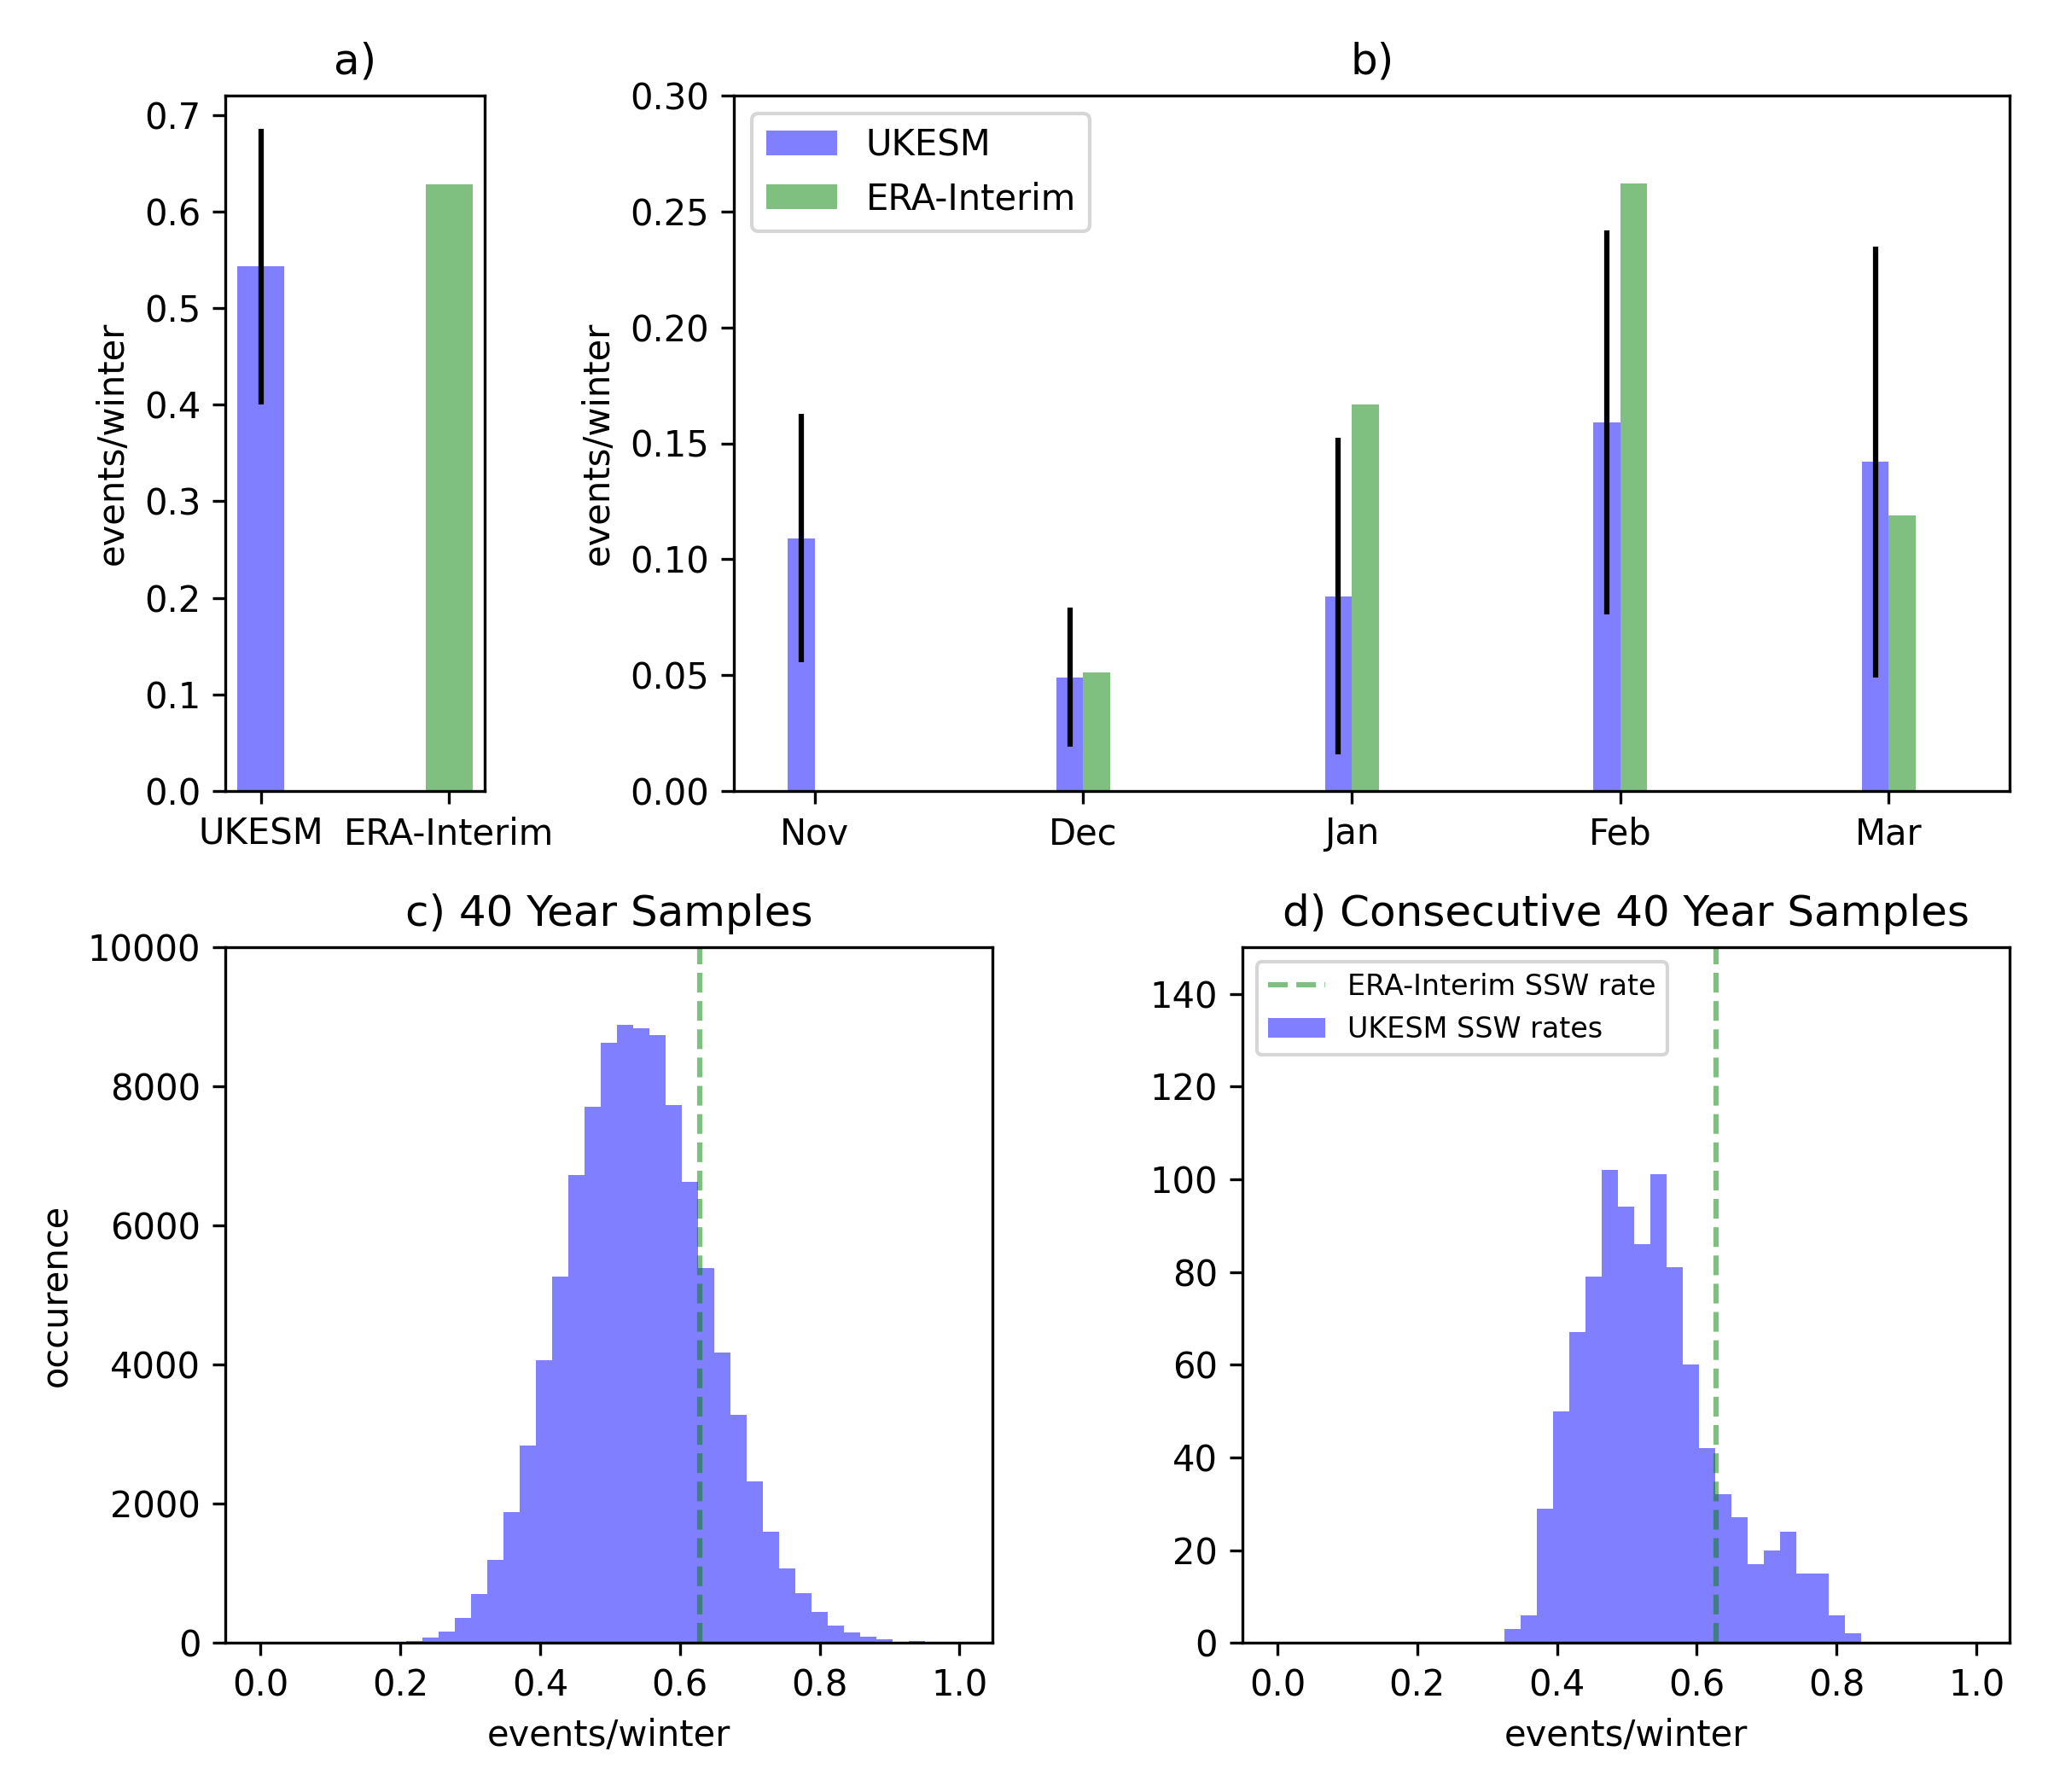
\includegraphics[width = 0.8\linewidth]{Figures/Figures-origins/SSW_hist_ERA_UKESM.png}
\caption[SSWs per NH winter season in the UKESM piControl and the ERA-Interim datasets.]{\textbf{a}: SSWs per NH winter season in the UKESM piControl and the ERA-Interim datasets. \textbf{b}: SSW rates separated by months. Error bars on a and b are derived using a bootstrap re-sampling method in which random selections of 40 years (the length of the reanalysis dataset) are chosen from the SSW data and the SSW rate recorded to build a PDF of events per season. 100000 such re-samples are carried out and the 95 and 5 percentile values are used as error bounds. This PDF is shown in blue bars in panel \textbf{c}. \textbf{d}: PDF of SSW rates in consecutive 40 year intervals of the UKESM simulation (blue bars). The SSW rate in ERA-Interim is indicated by the green dashed line in panels c and d.}
\label{fig:SSW_histogram}
\end{center}
\end{figure}

The model exhibits variability in SSW frequency comparable to observations, including both hiatus and consecutive SSW intervals. Figure \ref{fig:SSW_series_sample} shows a sample 40-yr interval of the polar vortex zonal wind strength and SSW occurrence from the UKESM simulation compared with a similar length from the ERA Interim reanalyses. An extended interval of mainly westerly anomalies indicating a strengthened vortex and lack of SSWs can be seen towards the end of the 40-yr interval, similar to the 1990s in ERA-Interim when only 2 SSW events were recorded in the decade. The simulation contains 8 such hiatus intervals with at least 10 consecutive years with no SSWs, the longest of which lasts 16 years. On the other hand, the simulation only contains 2 intervals in which 10 consecutive years exhibit at least 1 SSW. However, if the threshold interval width for identifying hiatus and consecutive-SSW intervals is shortened from 10 to 5 years, then 9 consecutive-SSW intervals and 25 hiatus intervals are found. These statistics indicate that UKESM is not only able to reproduce the mean state characteristics of SSW events but also decadal-scale variations in SSW rate, underlining its  suitability for this study. 

The second major mode of stratospheric variability is the QBO at equatorial latitudes which is present at all times of the year. Figure \ref{fig:equatorial_U_sample} shows the equatorial wind time-series from a sample 40-yr interval of the simulation compared with the ERA-Interim dataset. The mean period of the oscillation is longer than observed, at $\sim$38 months compared to $\sim$28 months in ERA-Interim \citep{kawataniRepresentation2016}. As a result the vertical shear zones descend less rapidly than observed. There is also a westerly bias at low levels where the QBO-E phase does not extend sufficiently deep into the lower stratosphere, which is a common bias in many models \citep{bushellEvaluation2020b}. The descending shear zones also appear more regular than observed but there is nevertheless some evidence of decadal-scale variations e.g. in the degree of stalling at 30\ hPa, although not as pronounced as in the observations.

\begin{figure}[h!]
\begin{center}
\noindent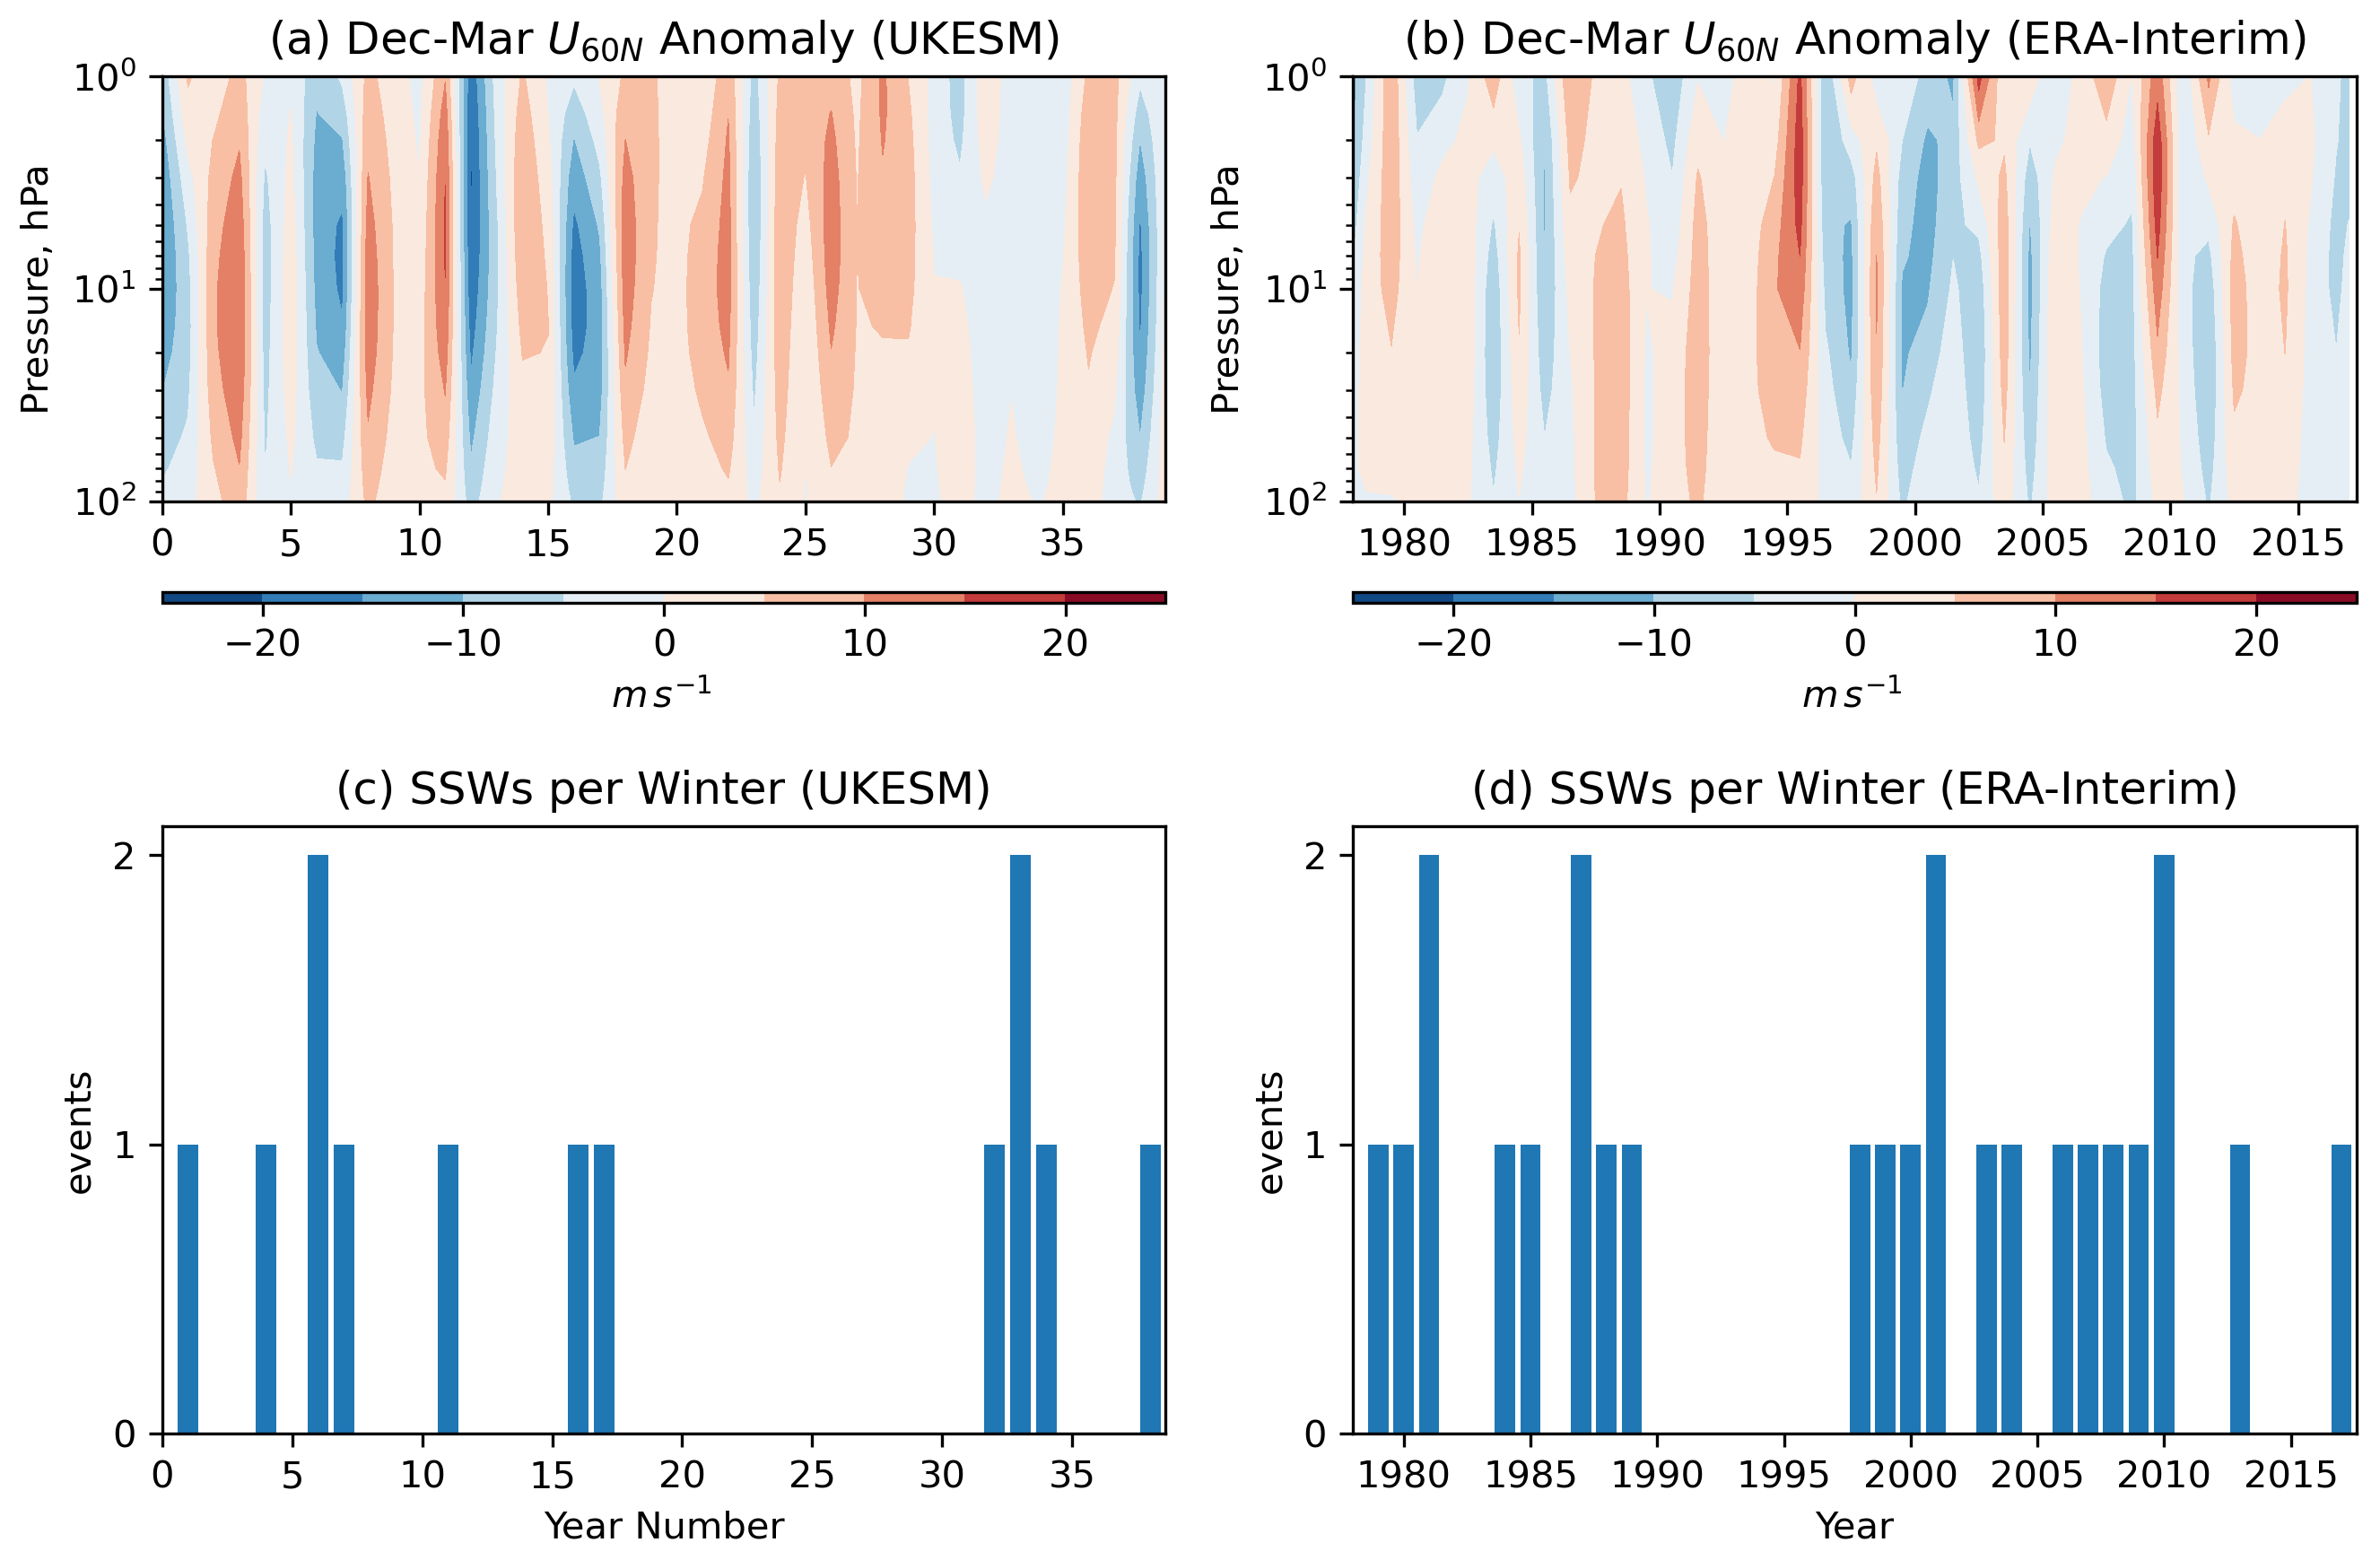
\includegraphics[width = \linewidth]{Figures/Figures-origins/SSW_series_ERA_UKESM.png}
\caption[Vortex ZMZW and SSW time series from UKESM pi-control and ERA-Interim]{\textbf{(a, b)}: Dec-Mar annual mean ZMZW anomaly from the climatological mean at 60$^\circ$\,N from a 40 year sample from the pre-industrial control simulation of UKESM \textbf{(a)} and the ERA-Interim dataset between 1979 and 2018 \textbf{(b)}. \textbf{(c, d)}: Time series of SSWs recorded per winter season in the same datasets.}
\label{fig:SSW_series_sample}
\end{center}
\end{figure}

%---------------------------------------------------------------

\begin{figure}[h!]
\begin{center}
\noindent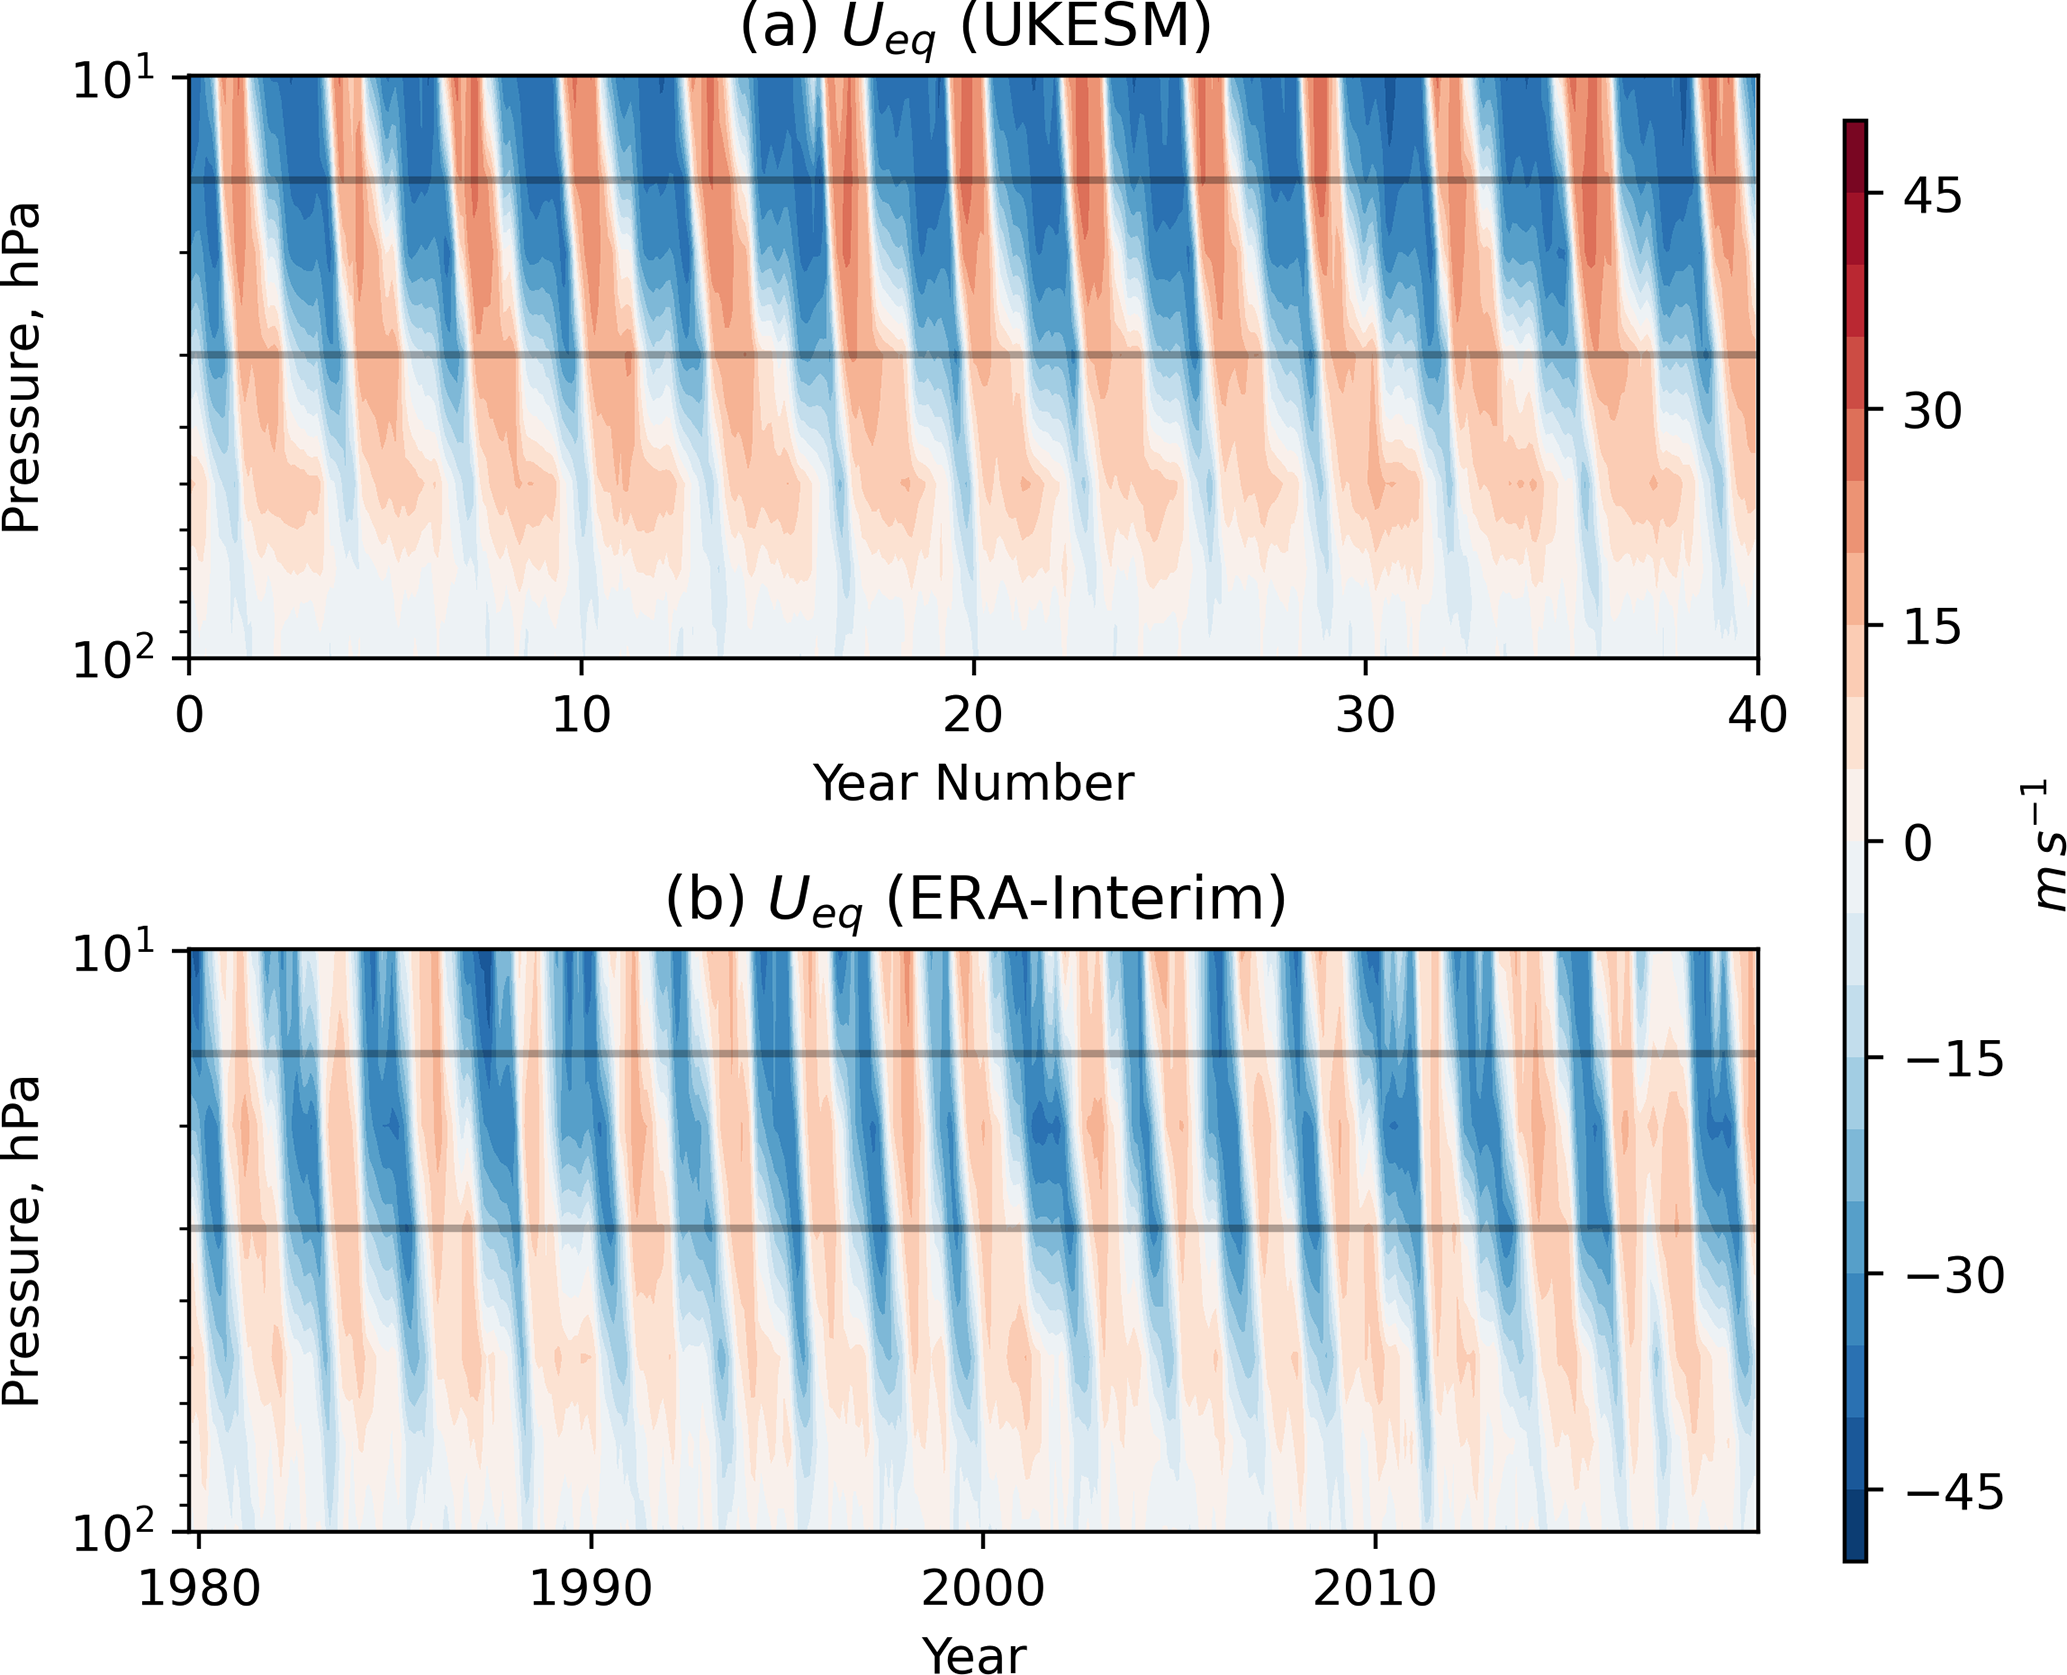
\includegraphics[width = 0.8\linewidth]{Figures/Figures-origins/equatorial_U_UKESM_ERA.png}
\caption[Time-height profiles for equatorial ZMZW from UKESM and ERA-Interim.] {ZMZW averaged between 5$^{\circ}$\,S--5$^{\circ}$\,N latitude from from a 40 year sample of the pre-industrial control simulation of UKESM \textbf{(a)} and the ERA-Interim dataset between 1979 and 2018 \textbf{(b)}. Horizontal lines mark the 15\,hPa and 30\,hPa levels between which the deep QBO metric employed by \cite{andrewsObserved2019d} is defined.}
\label{fig:equatorial_U_sample}
\end{center}
\end{figure}


%---------------------------------------------------------------

There is evidence of coupling between the two major modes of stratospheric variability in the model, giving rise to a Holton-Tan relationship \citep{ansteyHighlatitude2014b}. Figure \ref{fig:holton_tan_comp} shows height-latitude cross-sections of NH winter zonal wind differences between QBO E-W composites defined at various equatorial levels. The familiar pancake structure of alternating easterly / westerly differences is present at equatorial latitudes, indicative of the QBO phase but there is also a response at high latitudes. In good agreement with observations the largest high latitude response amplitude is seen when  the QBO is defined at 50hPa, with anomalously weaker polar vortex strength in QBO-E than in QBO-W years. Higher levels (15\,hPa and 20\,hPa) show little significant QBO-vortex coupling. For comparison we also show in figure \ref{fig:holton_tan_comp} the composite different response for QBO composites selected on the basis of the average QBO winds over a greater depth of the equatorial atmosphere (15-30 hPa and 20-50 hPa). We note that while this QBO definition will select some of the same years as in the separate single-level composite definitions, it is specifically designed to identify only QBO  phases that have extended vertical coherence, following \citep{graySurface2018b} and \cite{andrewsObserved2019d}, so the resulting composite  differences in figure 4 will not necessarily be an average of the corresponding single-level differences. Interestingly, the 15--30 hPa deep-QBO selects years that exhibit not only a weaker polar vortex in QBO-E but also a weaker sub-tropical tropospheric jet (see 200 hPa, 30--40N). This results in a more coherent response in the mid-latitude troposphere and at the surface, in excellent agreement with the results of \cite{graySurface2018b} and \cite{andrewsObserved2019d}. 

%---------------------------------------------------------------

\begin{figure}[h!]
\begin{center}
\noindent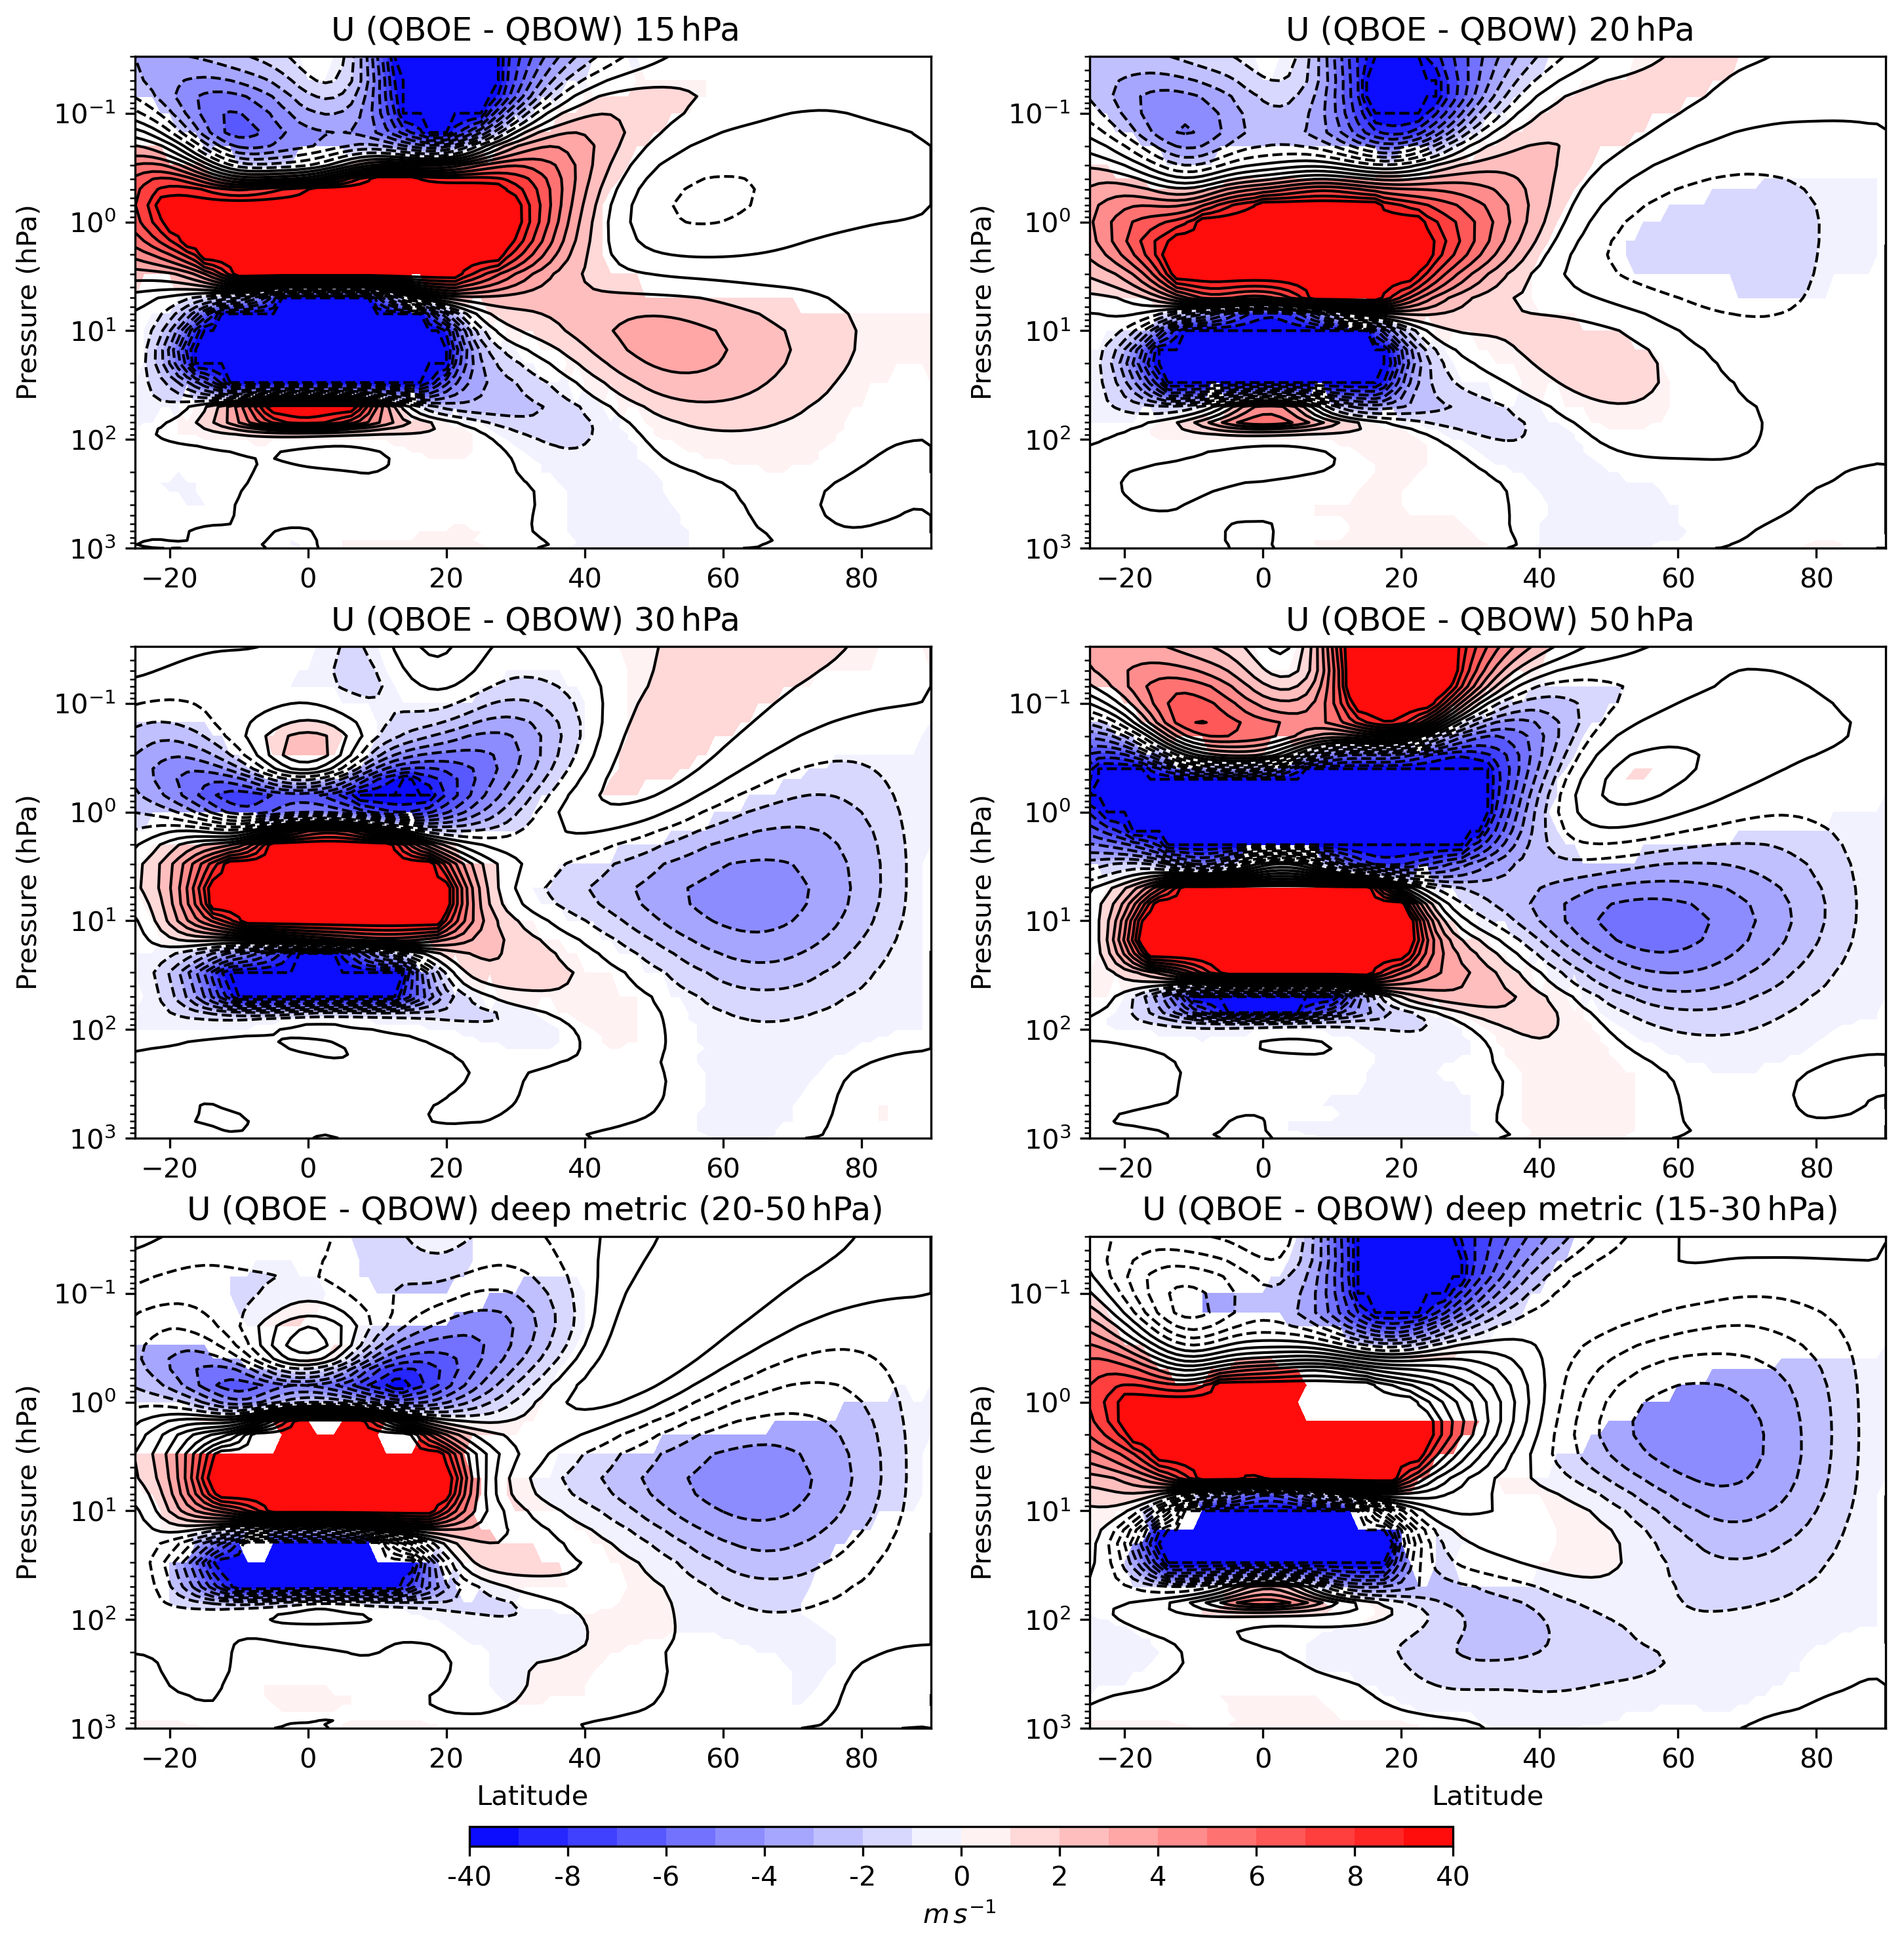
\includegraphics[width = 0.85\linewidth]{Figures/Figures-origins/holton_tan_composites.png}
\caption[ZMZW composite differences between QBO phases in UKESM pi-control.]{Dec-Mar ZMZW composite differences between QBO East and QBO West phases evaluated in Sep-Oct at individual levels as well as using the deep QBO metric. The phase of the QBO is defined any Sep-Nov equatorial ($5^{\circ}$\ S--$5^{\circ}\ $N average) ZMZW that exceeds a magnitude of 5\ m\,s$^{-1}$. Coloured shading indicates differences significant above the 95\% confidence level under a 2 tail student’s t-test.}
\label{fig:holton_tan_comp}
\end{center}
\end{figure}

The presence of the Holton-Tan relationship is also seen in the modelled frequency of SSWs (figures 5). Significantly higher rates are observed in QBO-E winters than QBO-W. Also notable is the asymmetry in abundance of QBO-E and QBO-W winters - nearly twice as many QBO-E winters are observed compared to QBO-W under all phase definitions (figure 5, legends). This suggests an element of phase locking between the QBO and the seasonal cycle possibly associated with seasonally variations in the strength of mean equatorial upwelling or mid-latitude planetary wave forcing in winter \citep{pascoeQuasibiennial2005b, gruzdevTwo2000b, rajendranSynchronisation2016b} resulting in QBO phase transitions that occur preferentially in certain months. 

\begin{figure}[h!]
\begin{center}
\noindent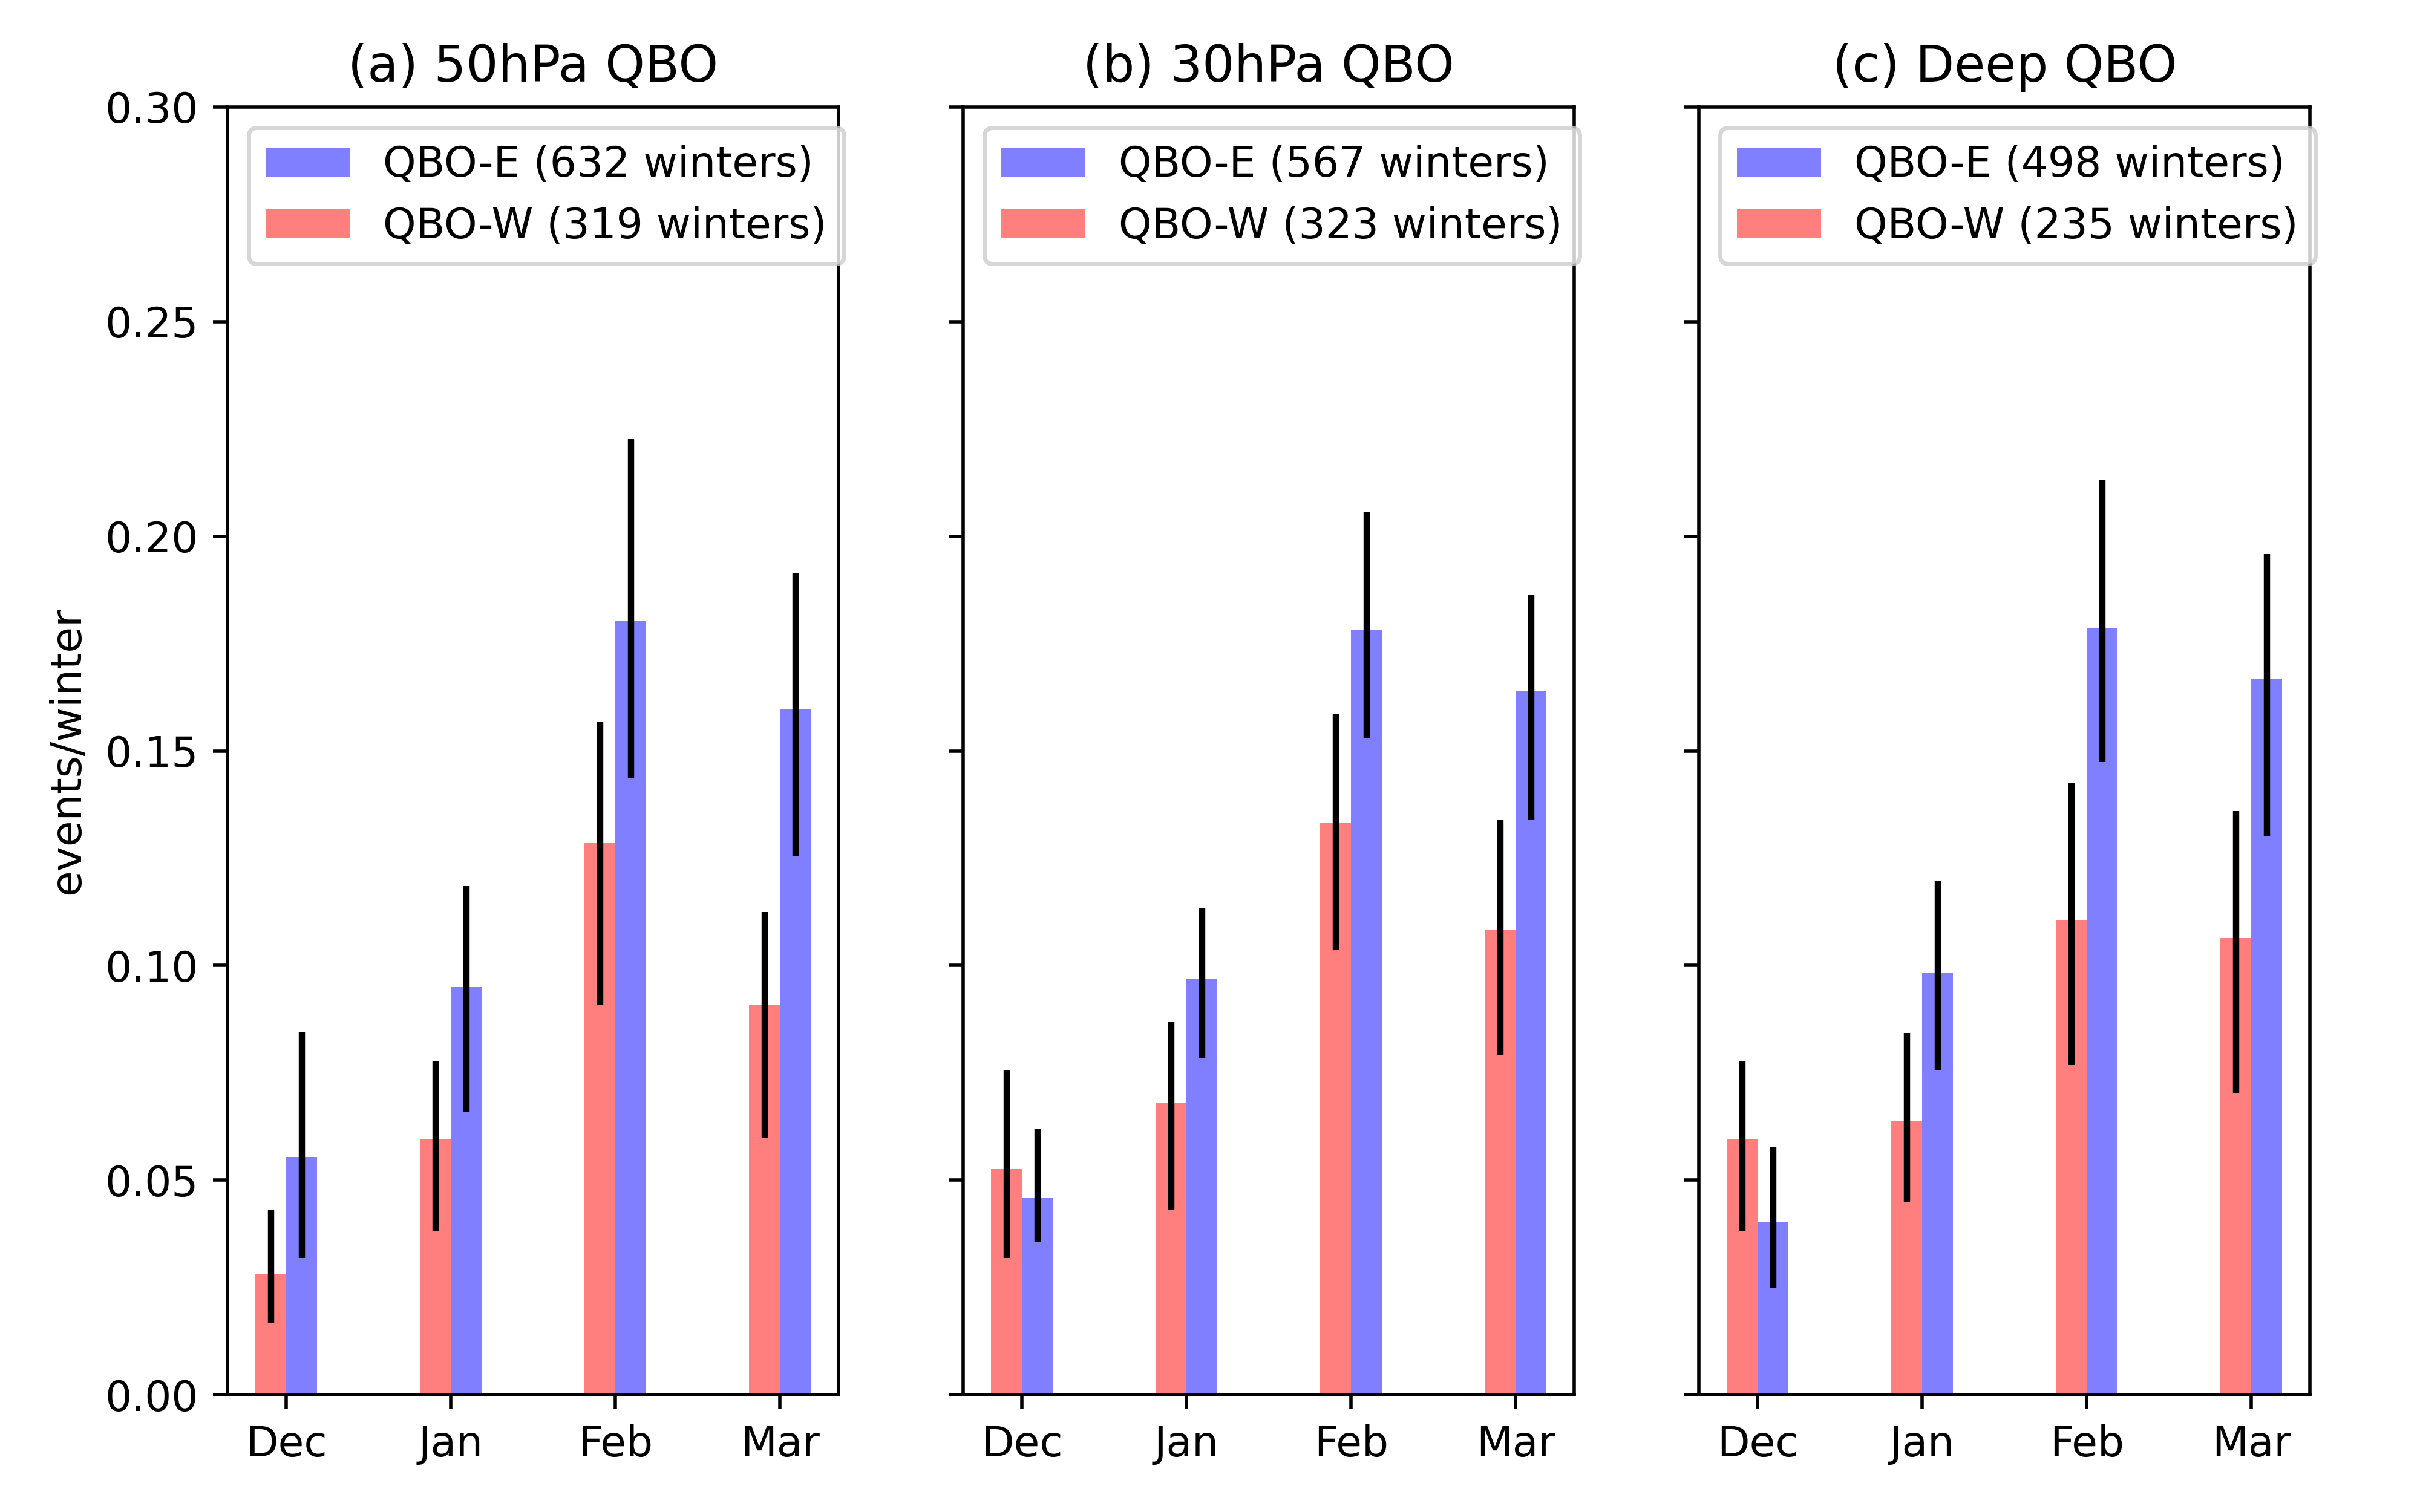
\includegraphics[width = 0.9\linewidth]{Figures/Figures-origins/SSW_histograms_QBOphases.png}
\caption[Histogram of SSWs per winter in different QBO phases in UKESM.]{SSWs per winter season for years exhibiting QBO-E and QBO-W conditions in early winter (Sep-Nov) defined on different pressure levels (a,b) as well as using the deep metric (c), the vertical mean between 15 and 30\,hPa defined in \cite{andrewsObserved2019d}. The QBO phase is defined as any Sep-Nov equatorial ($5^{\circ}$\ S--$5^{\circ}\ $N average) ZMZW that exceeds a magnitude of 5\ m\,s$^{-1}$. Error bars on all plots are derived using the same bootstrapping method outlined in figure \ref{fig:SSW_histogram}}
\label{fig:SSW_hist_QBO_phase}
\end{center}
\end{figure}

There is also evidence of in-season coupling between the vortex and phases of ENSO as well as the AL. Composites of ZMZW under different Ni\~{n}o3.4 conditions (figure \ref{fig:ZMZW_comp_ENSO_AL}a, b) shows a response from vortex winds to the 2 types of anomalous ENSO behaviour. The vortex appears significantly stronger under La Ni\~{n}a conditions and weaker under El Ni\~{n}o, a result which is consistent with numerous studies from both observations and other models (see section \ref{sec:external_influence_SSTs}). As is noted in \cite{polvaniDistinguishing2017b}, the vortex response to ENSO in the model appears more linear than those generally found in observation based studies; the magnitude of responses to each phase is similar. In contrast, the vortex response to different signs of the AL (figure \ref{fig:ZMZW_comp_ENSO_AL}c, d) index is highly asymmetric. The vortex is considerably weakened under anomalously negative AL values (corresponding to a more intense Aleutian Low) while the positive AL phase only leads to a marginal strengthening in vortex winds. This may me due to the proposed mechanism by which the AL influences the vortex, via alteration of planetary wave propagation into the stratosphere. This provides modulation of the weakening mechanism of the vortex under negative AL but not a strengthening under positive - simply an absence of wave fluxes. Nevertheless, these AL composites are consistent with the findings of studies outlined in \ref{sec:external_influence_AL} which report a weakened vortex under negative AL conditions. Both sets of composites indicate that the model is able to reproduce expected in-season vortex responses from these key modes of surface variability, further suggesting its suitability for an analysis of external influence on the vortex from these modes on multi-decadal timescales. 

\begin{figure}[h!]
\begin{center}
\noindent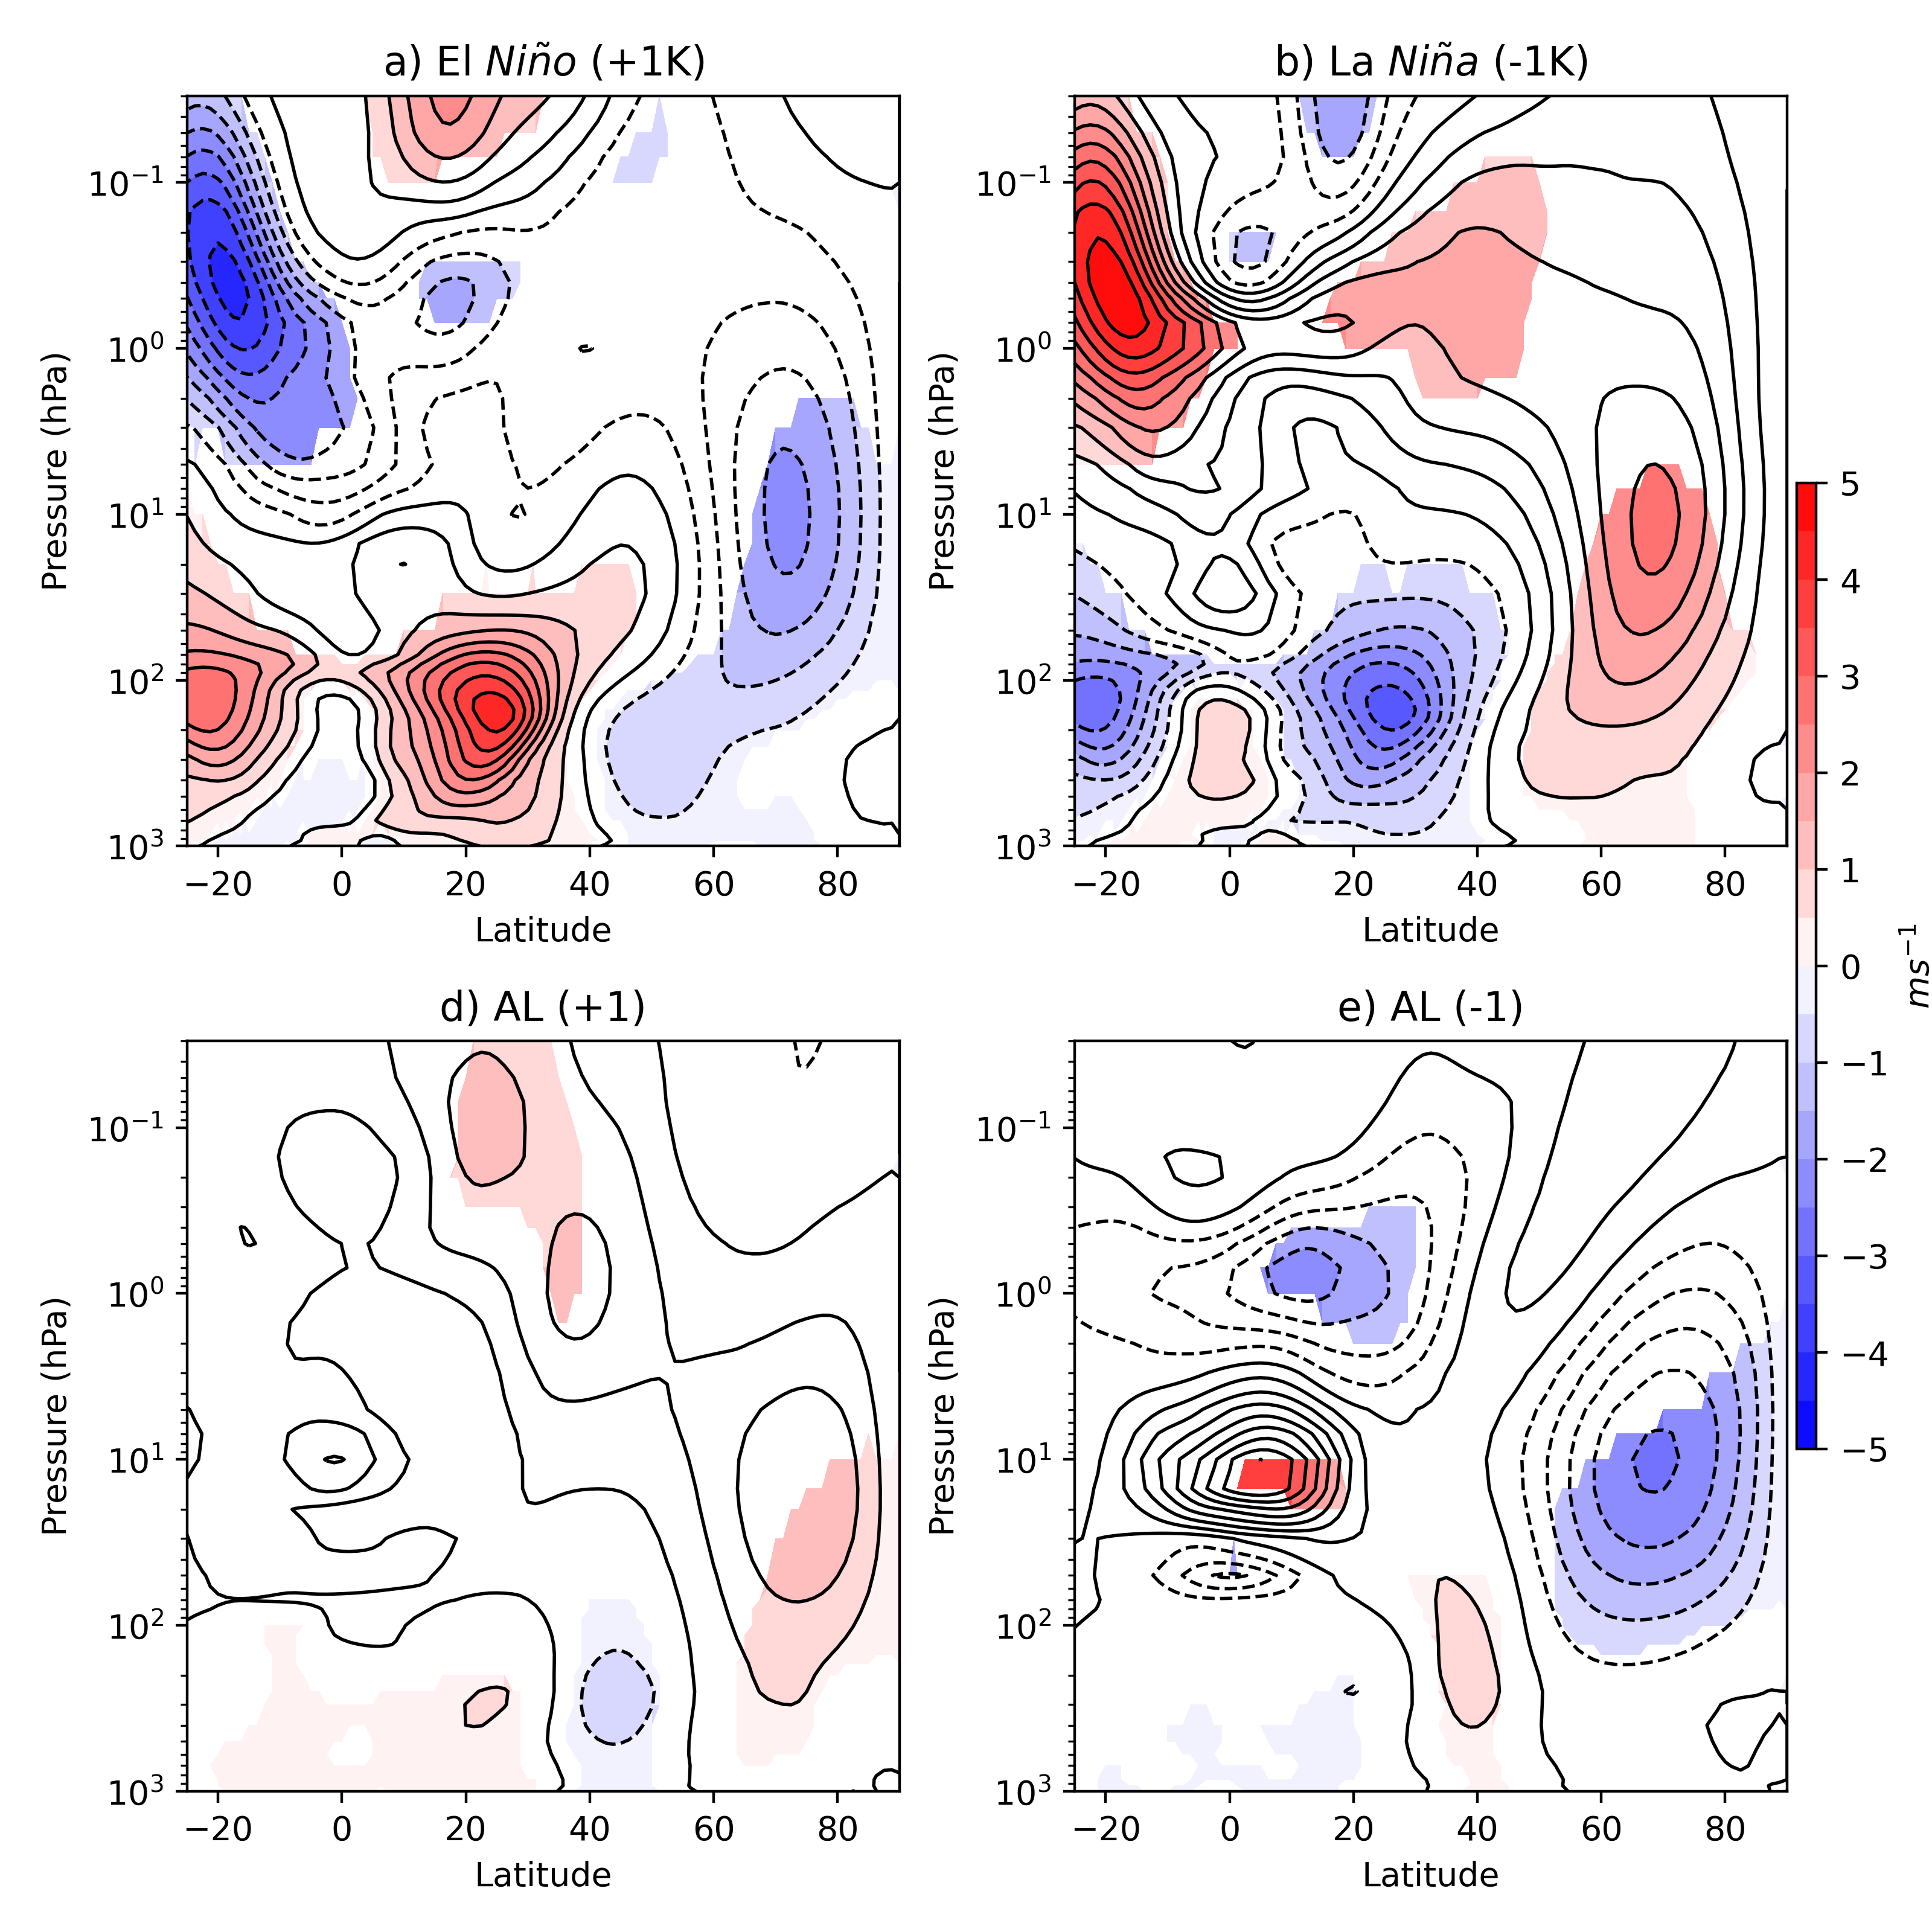
\includegraphics[width = 0.75\linewidth]{Figures/Figures-origins/ZMZW_comps_ENSO_AL.png}
\caption[Dec-Mar ZMZW anomaly composites for different phases of ENSO and the AL]{Dec-Mar ZMZW anomaly composites for positive (El Ni\~{n}o) and negative (La Ni\~{n}a) phases of the Ni\~{n}o3.4 index evaluated in Sep-Nov (a, b) and the Aleutian low index evaluated in Dec-Feb (c, d). The phase of Ni\~{n}o3.4 is defined as an SST anomaly of greater magnitude than 1K and the AL phase as an index value derived using the principal component based definition of greater magnitude than 1. Coloured shading indicates anomalies significant above the 95\% confidence level under a 2-tailed student’s t-test.}
\label{fig:ZMZW_comp_ENSO_AL}
\end{center}
\end{figure}



\section{Regression Analysis}
We next employ a multi-linear regression analysis to measure the relative contributions to the time-series of SSWs per year (as in figure \ref{fig:SSW_series_sample}) from the QBO, ENSO and the Aleutian low. The results from this analysis are summarised in table 1.  Sensitivity experiments were performed to identify the optimum averaging lagged response by the vortex to each index: the deep 15-30 hPa QBO index and Ni\~{n}o3.4 indices were both defined using early winter (Sep-Nov) averages while the AL index was defined using Dec-Mar averages. The coefficients are all significant to the 95\% level but are relatively small and the $R^2$ score is only 0.047 indicating these variables account for only a small portion of the variability in the SSW timeseries. While results from this multi-linear regression analysis are easy to interpret, the approach does not directly tackle the problem posed in this study, that of multi-decadal variability in SSWs and its origins, for two main reasons. Firstly, regression analysis assumes stationarity i.e. it provides a measure of stationary contributions to variability and will only highlight signals that are relatively persistent for the whole simulation. Secondly, it  analyses variability in the time series at all timescales simultaneously, so that the results are dominated by the timescales with larger amplitude variations.  This means that the results in table 1 are most likely dominated by the shorter (inter-annual) timescales and any small amplitude variations at longer timescales will not be revealed. The latter can be addressed to some extent by smoothing or filtering the time-series, as discussed in the next section, but this requires prior knowledge of which frequencies are of interest. Furthermore, co-variability in predictor indices of a regression model may lead to spurious coefficients. This may be an issue here as \cite{raoModulation2019d} note correlations between ENSO and the AL. The variance inflation factor is a measure of the degree to which each regression coefficient is altered by predictor co-variations. the VIF for each predictor is greater than 1 indicating a moderate degree of co-variation with other predictors \citep{akinwandeVariance2015b} which may further hamper the efficacy of this regression method. An alternative and superior approach to this problem employs wavelet analysis, described more fully in the next section, which successively examines different frequency intervals to identify the presence of signals thus avoiding dominance by one particular frequency, and also measures the time evolution of the signal so that non-stationary signals can also be identified. 

\begin{table}[h!]
\centering
\begin{tabular}{|p{3cm}||p{3cm}|p{3cm}|}
 \hline
 \multicolumn{3}{|c|}{SSW regression}\\
 \hline
 Regression Variable& Coefficient& p value\\
 \hline
 Ni\~{n}o3.4  & 0.1625$^+_-$0.035& 0.0002\\
 AL  &   -0.0927$^+_-$0.04  & 0.048\\
 deep QBO  & -0.1993$^+_-$0.03&0.0001\\
 \hline
 \end{tabular}
\begin{center}
\caption{Summary of results from regression analysis of SSWs per NH winter time series.}
\label{table:regression_SSW}
\end{center}
\end{table}

%---------------------------------------------------------------

\section{Long-term Variability of the Polar Vortex}
A more comprehensive assessment of the long-term variability of SSWs can be made using a wavelet power spectrum approach outlined in section \ref{sec:Wavelet_Analysis}. We count the number of SSWs in each winter season (Dec-Mar) and calculate the corresponding wavelet power spectrum, shown in figure \ref{fig:SSW_series_wavelet}. As described above, the analysis highlights the presence of power in the signal as a function of frequency (period in years, along the y-axis) and as a function of time (year of simulation along the x-axis). As expected, there is an intermittent but relatively persistent signal with period around 2-4 years throughout the simulation, corresponding to the period of the QBO which supports the presence of a Holton-Tan relationship between the QBO and the polar vortex in the model. The so-called 'global power spectrum' (i.e. the time average of the wavelet spectrum) shown on the right of figure \ref{fig:SSW_series_wavelet} shows that the signal is on the boundary of the 95\% statistical significance. Other signals at periods near 20-30 years are similarly intermittent and manifest as a peak in the time-averaged spectrum that is also near the 95\% significance boundary. There is also a feature at periods between $\sim$60-90 years in the interval between 400-800 yrs. This feature shows statistical significance (based on comparisons between power in the spectrum and that of an AR1 process with the same autocorrelation structure as the series being analysed) for around 300 years of the 1000-yr simulation but does not cross the significance threshold for the time-averaged spectra. There is a possible limitation of this wavelet methodology due to the discrete nature of the time series being analysed (time points take values 0/1/2). The Morlet wavelet is a continuous function and, as a result, convolution with a highly discretised series may alias features on the resulting wavelet spectra. This limitation must be considered when drawing conclusions from the wavelet spectra and is discussed further below.

\begin{figure}[h!]
\begin{center}
\noindent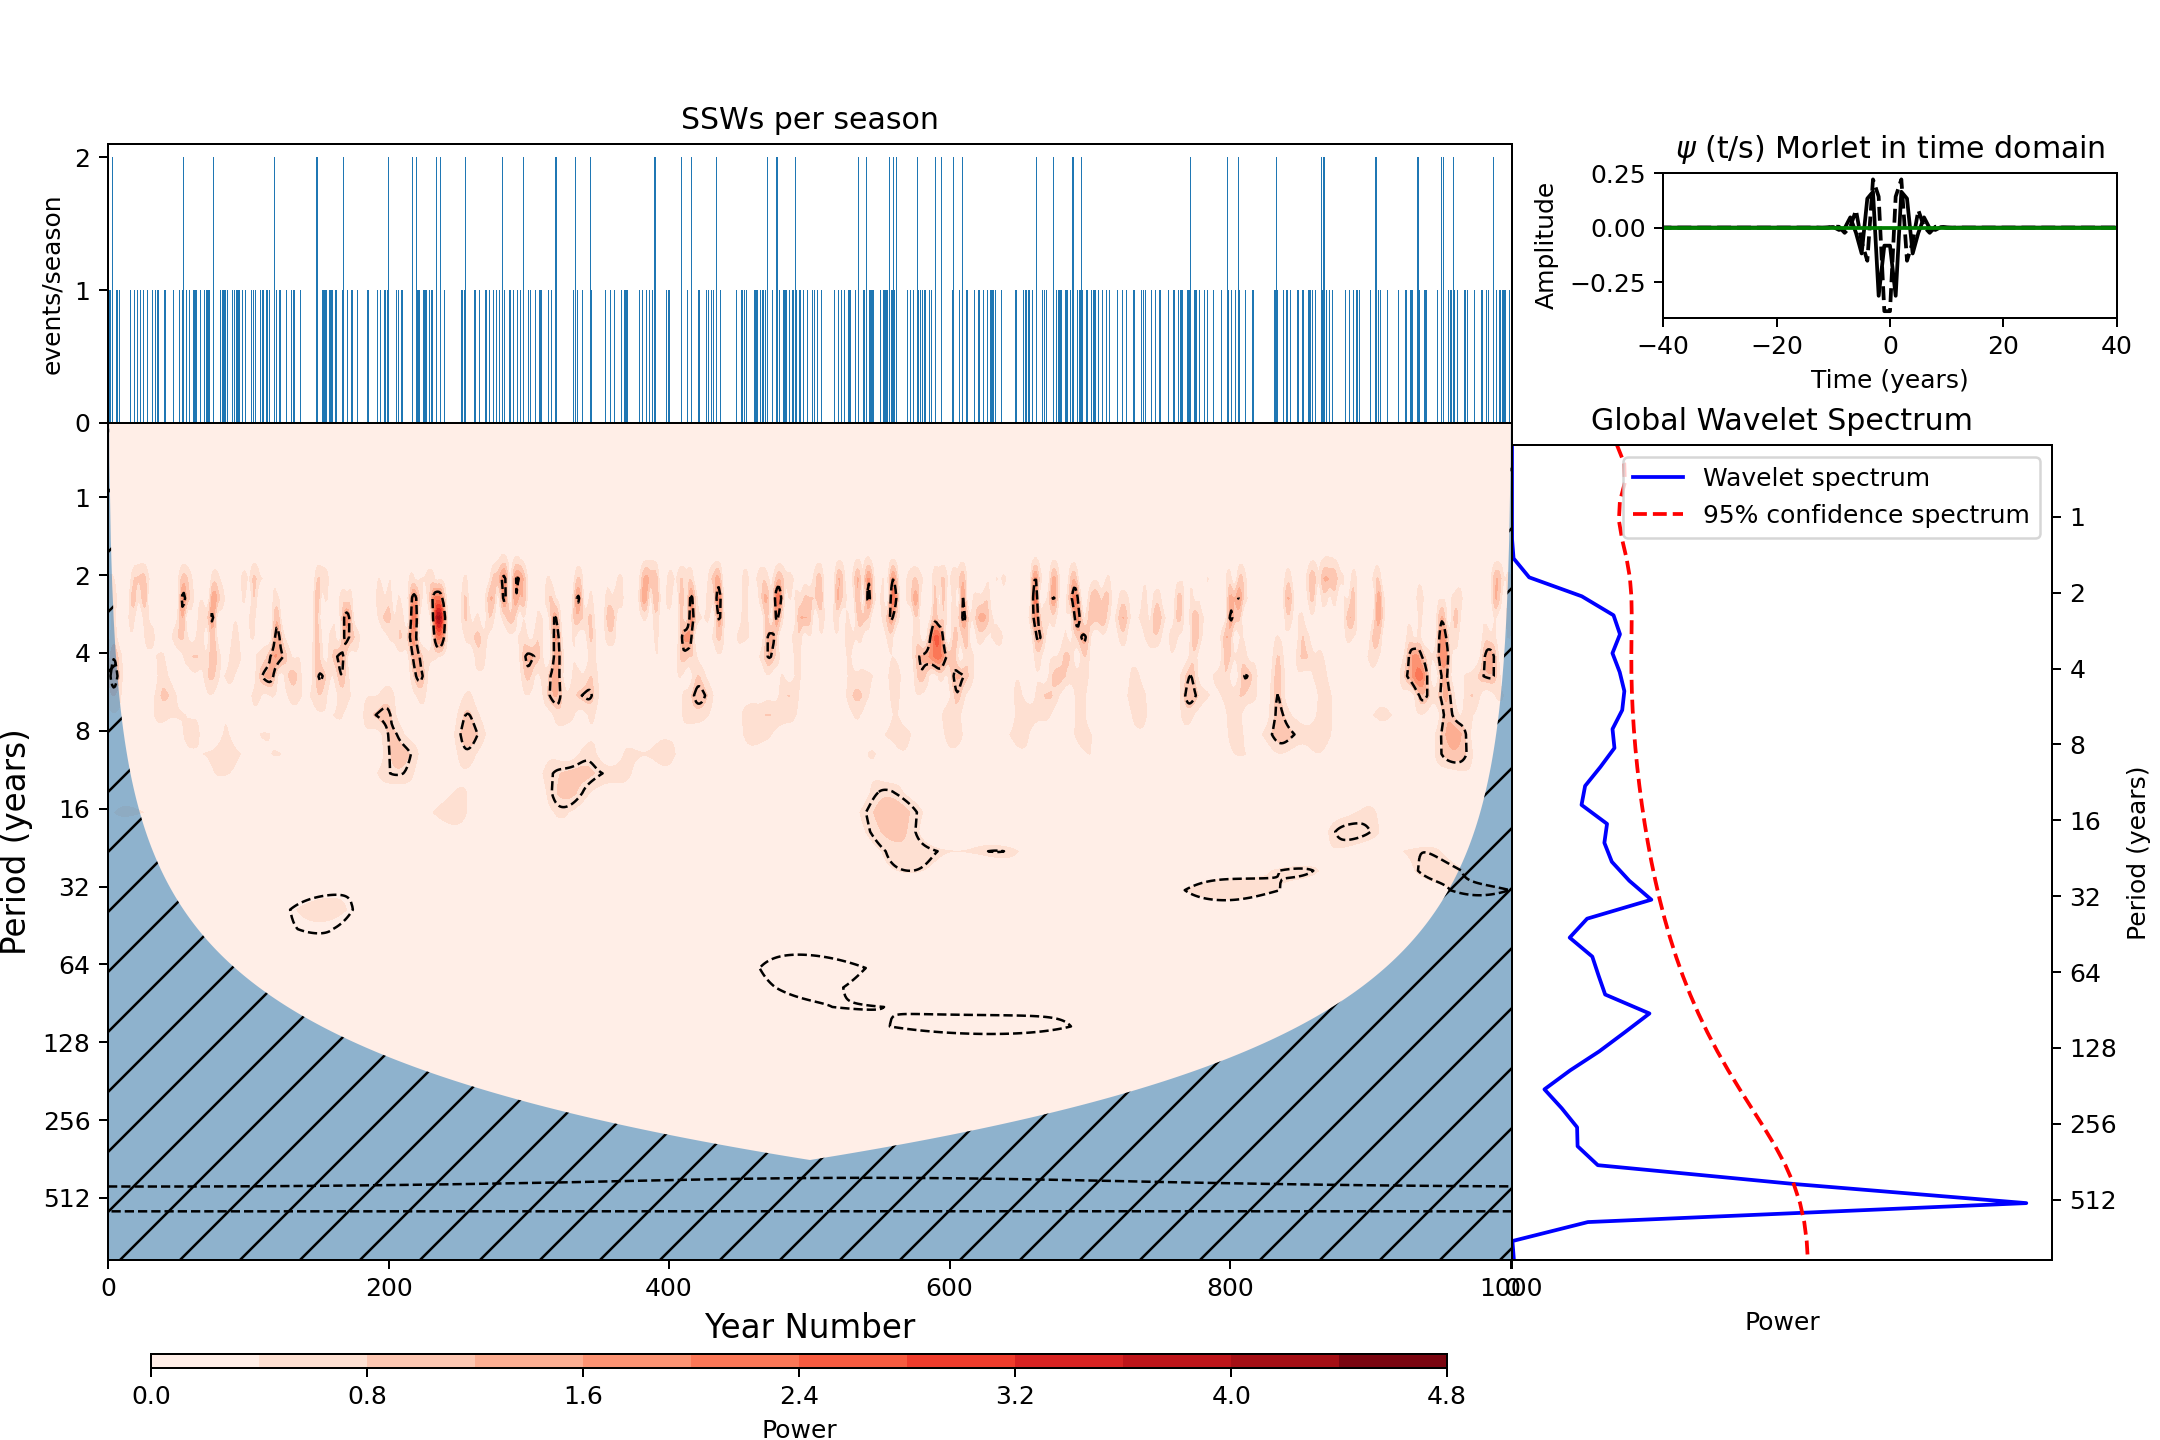
\includegraphics[width = 0.8\linewidth]{Figures/Figures-origins/SSW_wavelet.png}
\caption[Wavelet power spectrum for SSW time series in UKESM pi-control]{\textbf{Top left}: SSW events per Dec-Mar season in UKESM \textbf{Bottom left}: Wavelet power spectrum of time series in top left. Hatching represents area outside the cone of influence in which edge effects are significant and power should not be considered. Yellow contours represent the 95\% confidence level assuming mean background AR1 red noise. \textbf{Top Right}: Morlet wavelet used for the wavelet transform in the time domain. \textbf{Bottom right:} Global power spectrum, the wavelet power averaged over the whole simulation (blue line), and global 95\% confidence spectrum (red dashed line).}
\label{fig:SSW_series_wavelet}
\end{center}
\end{figure}

%---------------------------------------------------------------

The focus of this study is on the longer-term time variations to understand the source of variability characterised by hiatus intervals (no SSWs over an extended period) and consecutive-event intervals (at least one SSW every year for an extended period). We therefore apply low-pass filtering to the time series of SSWs per season using a 5-year rolling window and examine the spectral characteristics of this smoothed series (which we refer to henceforth as $SSW_{5yr}$). This averaging is similar to the standard practice of smoothing daily data to remove the noise associated with daily weather variations, thus isolating longer seasonal timescales. It also decreases the impact of the time series discretisation and therefore reduces the chance of introducing spurious spectral features on the wavelet power spectrum which could be otherwise encountered when analysing the un-smoothed time series.  

\begin{figure}[h!]
\begin{center}
\noindent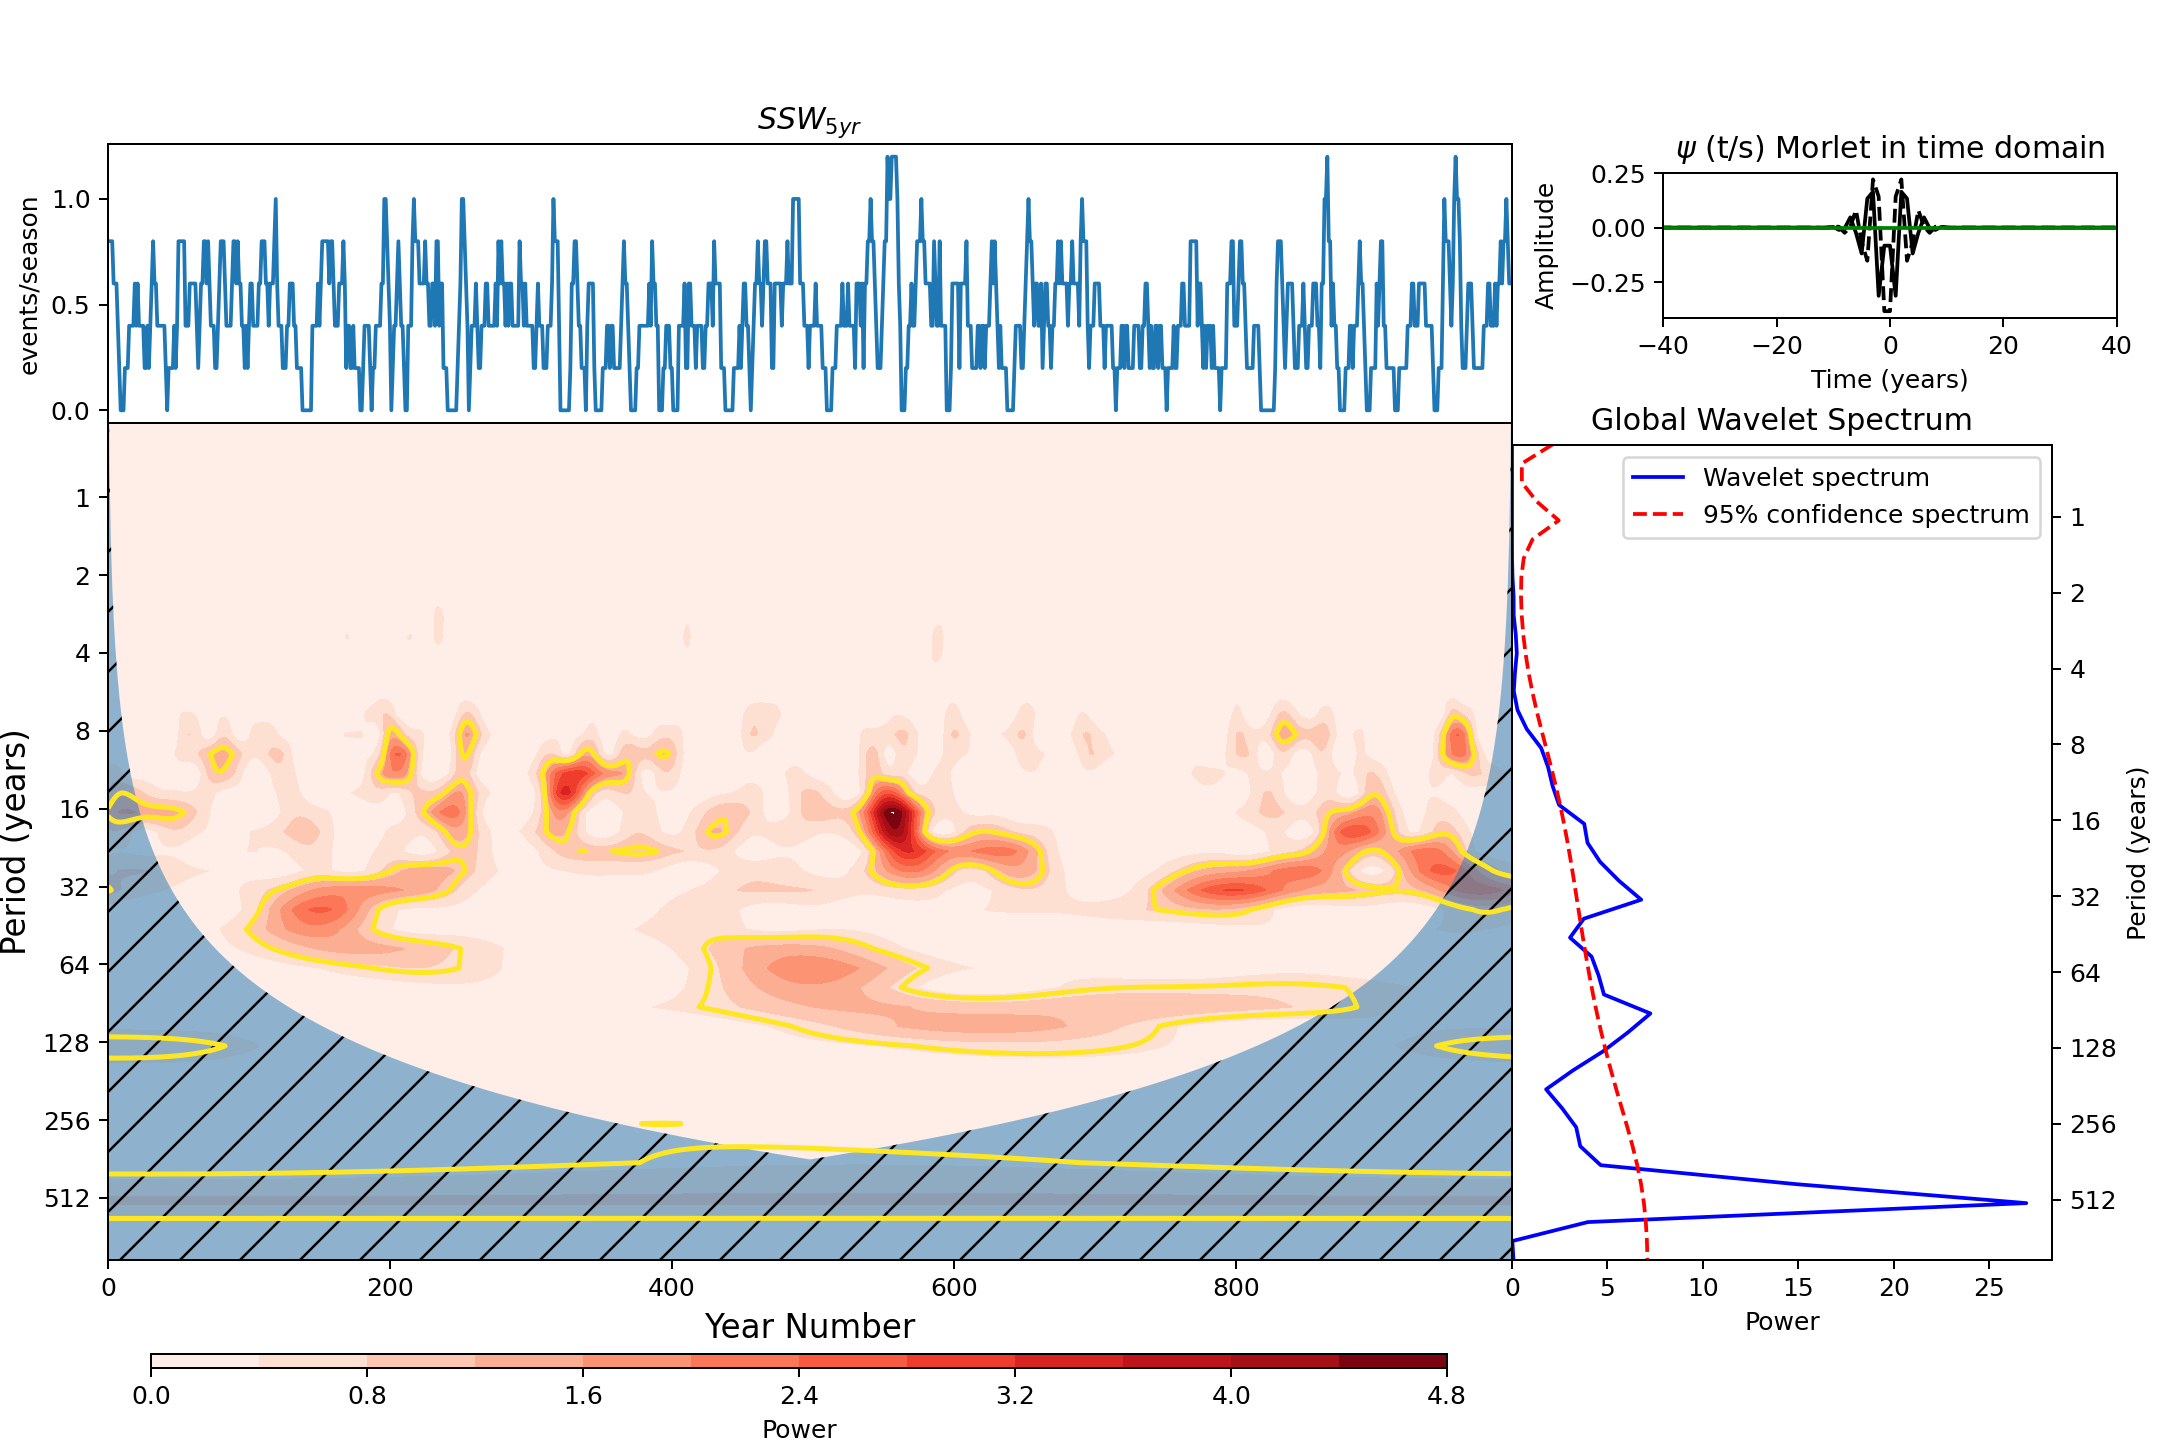
\includegraphics[width = 0.8\linewidth]{Figures/Figures-origins/SSW_wavelet_5_yr_wavelet.png}
\caption[Wavelet power spectrum for Dec-Mar 5 year mean SSW time series in UKESM pi-control]{\textbf{Top left}: SSW events per Dec-Mar season in UKESM smoothed using a 5 year running mean. \textbf{Bottom left}: Wavelet power spectrum of time series in top left. Hatching represents area outside the cone of influence in which edge effects are significant and power should not be considered. Navy contours represent 95\% confidence level assuming mean background AR1 red noise. \textbf{Top Right}: Morlet wavelet used for the wavelet transform in the time domain. \textbf{Bottom right:} Global power spectrum, the wavelet power averaged over the whole simulation, and global 95\% confidence spectrum.}
\label{fig:SSW_series_5yr_wavelet}
\end{center}
\end{figure}

%---------------------------------------------------------------
The wavelet power spectrum of $SSW_{5yr}$ (figure \ref{fig:SSW_series_5yr_wavelet}) shares many of the characteristics of the spectra of the un-smoothed series (figure \ref{fig:SSW_series_wavelet}), but the longer period signals are now more clearly evident, as expected. The $SSW_{5yr}$ wavelet spectrum shows the two broad regions of statistically significant maxima corresponding to signal periods of $\sim$20-30 years and $\sim$60-90 years, but with increased significance both locally and in the time-average. For example, the feature around 90 year period appears significant for 450 years in $SSW_{5yr}$ compared to 350 years before smoothing. One possible explanation for this increase lies in our definition of the significance level on power which is dependent on the lag-1 autocorrelation of the time-series. Introducing a 5 year averaging window will increase the autocorrelation, possibly leading to a less strict significance level. However, this is unlikely because the significance level is constructed using a red noise process with the same autocorrelation as the series. This means that for $SSW_{5yr}$, the threshold for 95\% confidence level increases with increasing period more steeply than in the un-smoothed case and yet the power exhibited at those long periods in $SSW_{5yr}$ nevertheless achieves higher statistical significance. This indicates that the smoothing has enhanced the visibility of a real signal in the $SSW_{5yr}$ time series that was less visible in the un-smoothed time-series. As a check for robustness, we also include the $SSW_{5yr}$ wavelet spectrum including the over-represented November SSW events (figure \ref{fig:SSW_series_5yr_NDJFM_wavelet}). it looks similar to  the spectrum shown in figure \ref{fig:SSW_series_5yr_wavelet} but contains more persistent power on the 8-32 year timescales. The feature noted about on the Dec-Mar $SSW_{5yr}$ wavelet spectrum on $\sim$60-90 years timescales is also present with persistent power for around 450 years of the simulation at these periods. We proceed with the Dec-Mar SSWs for the analysis of possible drivers of this variability as the cause of the November SSW bias in the model is not fully understood and may make attribution of signals more difficult. 


\begin{figure}[h!]
\begin{center}
\noindent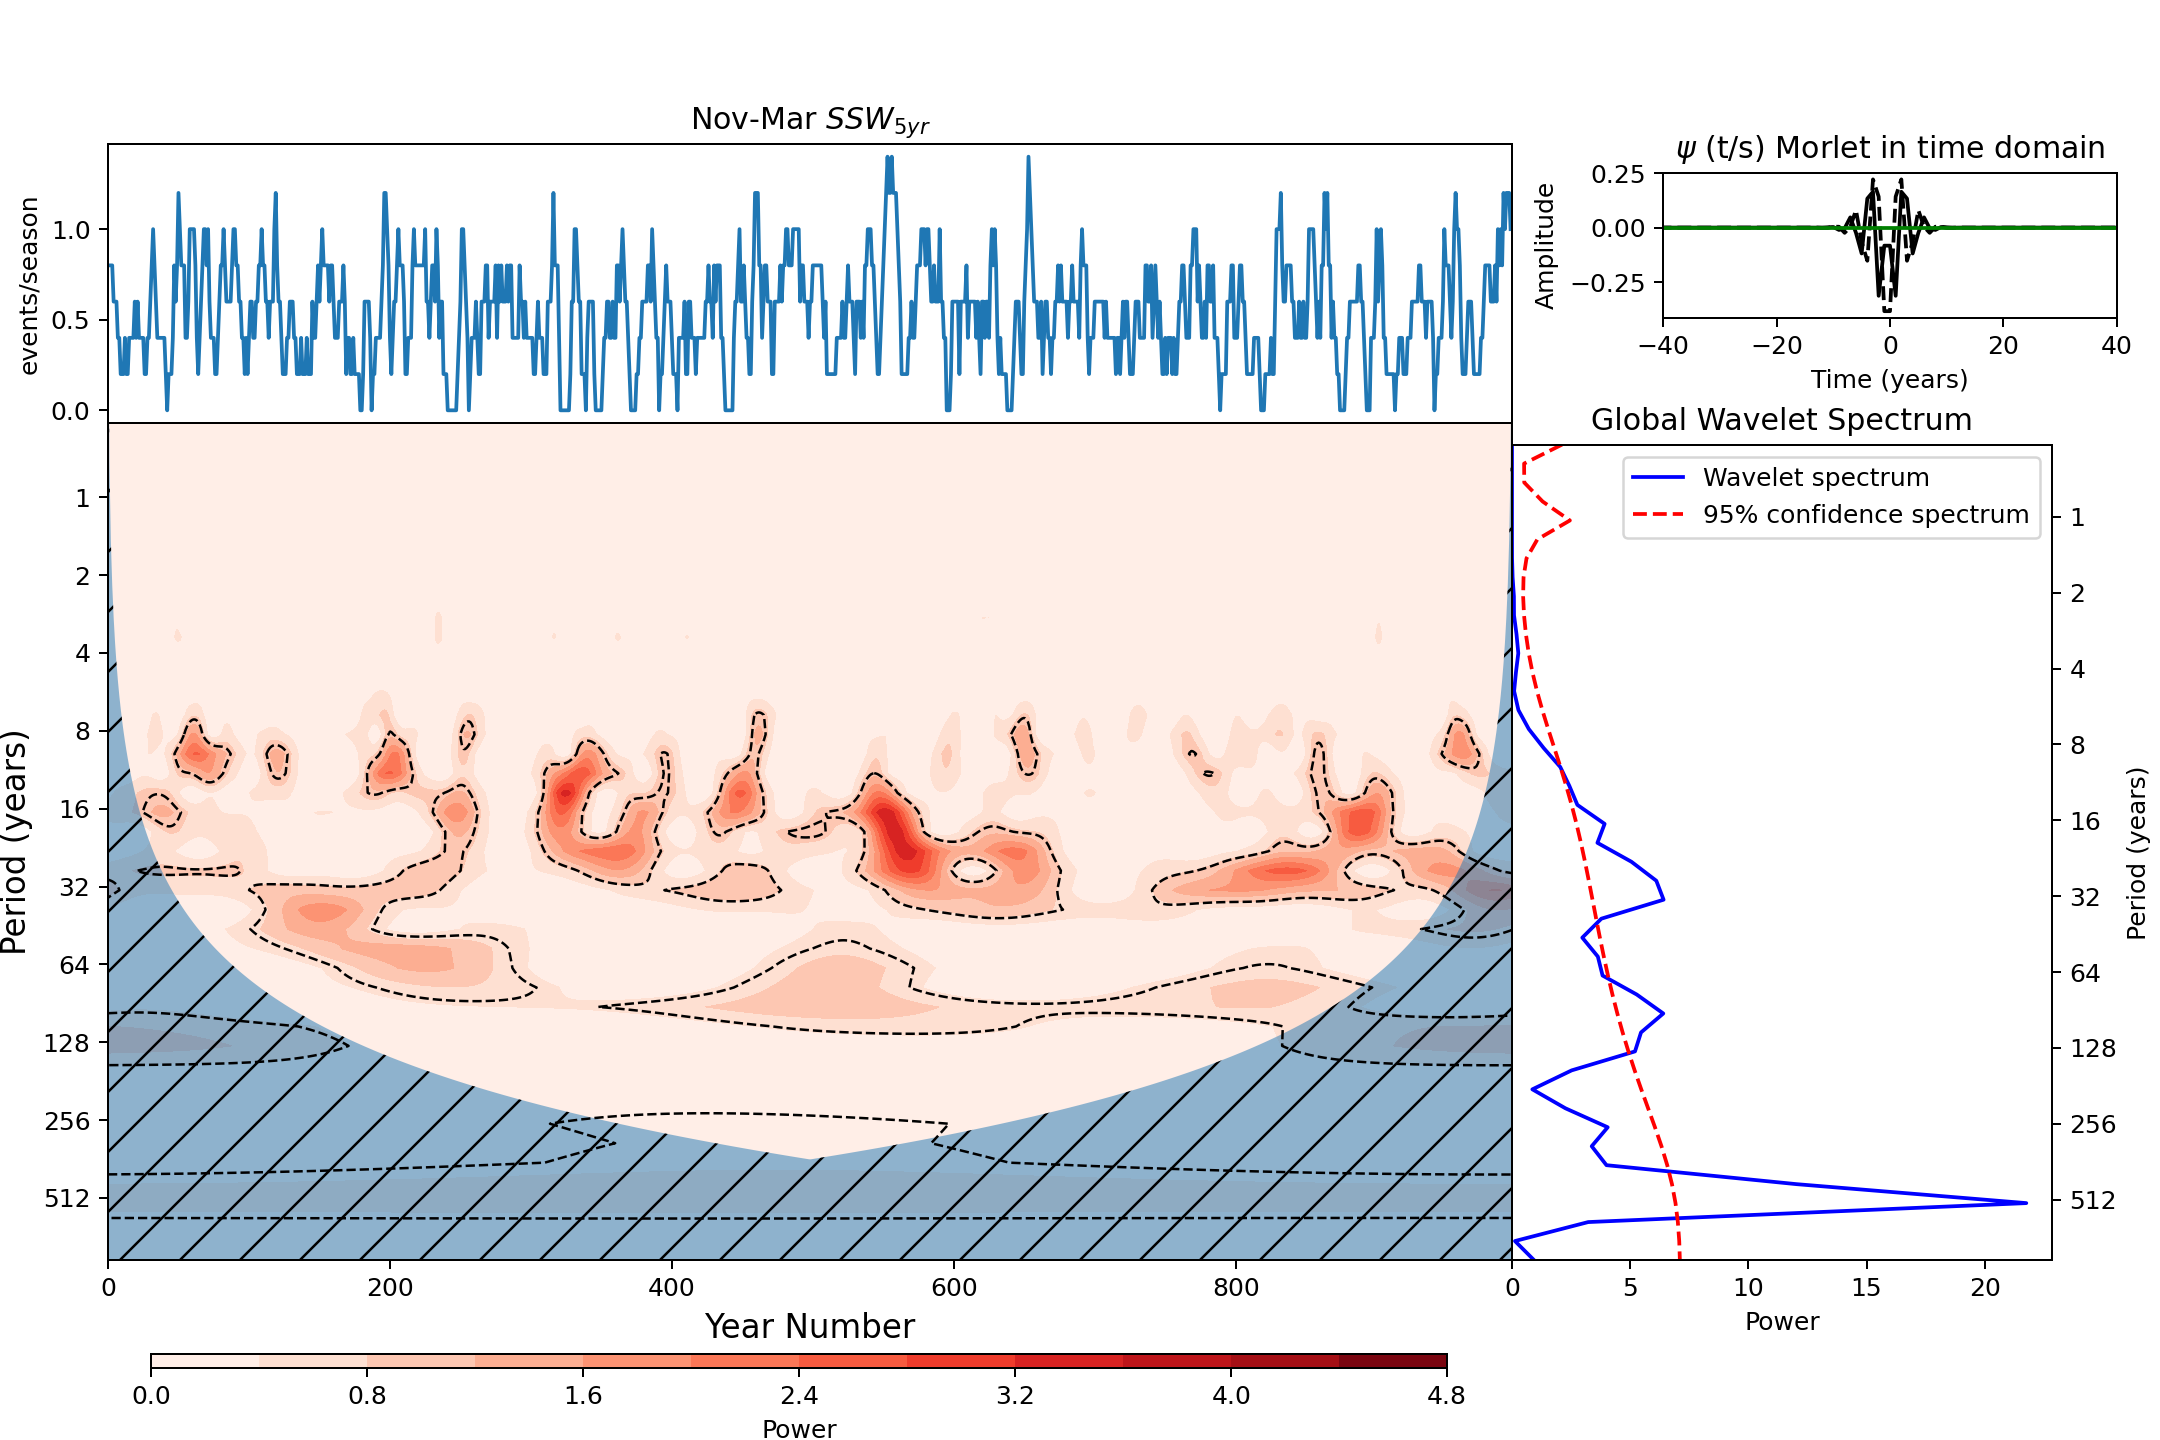
\includegraphics[width = 0.8\linewidth]{Figures/Figures-origins/SSW_wavelet_5_yr_NDJFM.png}
\caption[Wavelet power spectrum of Nov-Mar 5 year mean SSW time series in UKESM pi-control]{Like figure \ref{fig:SSW_series_5yr_wavelet} for the Nov-Mar SSWs per NH winter season timeseries smoothed with a 5 year rolling window.}
\label{fig:SSW_series_5yr_NDJFM_wavelet}
\end{center}
\end{figure}

%---------------------------------------------------------------


\section{Surface Forcing of Polar Vortex Variability}
In the absence of external forcing mechanisms such as greenhouse gas or anthropogenic aerosol forcing, the presence of long-term variability such as the 60-90 year periodicity seen in $SSW_{5yr}$ (figure \ref{fig:SSW_series_5yr_wavelet}) suggests a source of long-term internal variability from within the climate system. 

The most obvious potential driver of such long timescale variability is the ocean due to its high degree of thermal inertia. Previous work has identified coupling between tropical SSTs and the polar vortex, such as the relationship to ENSO conditions (see section \ref{sec:external_influence_SSTs}). The model exhibits an expected connection between ENSO and the vortex on interannual timescales indicated by the regression analysis results (table 1) and ZMZW composites for El Ni\~{n}o and La Ni\~{n}a winters (figure \ref{fig:ZMZW_comp_ENSO_AL}a, b). Figure \ref{fig:ENSO_wavelet} shows the wavelet power spectrum for the 5 year smoothed Sep-Nov ENSO 3.4 index as well as the cross power spectrum with $SSW_{5yr}$. We use the early NH winter ENSO index to capture the lagged response of the vortex to this mode of variability. The ENSO index is slowly varying so will likely remain in the same state between early and mid-winter. We also smooth the ENSO index for the purposes of calculating the cross spectrum with $SSW_{5yr}$. (The spectrum of the un-smoothed Ni\~{n}o3.4 index is provided in figure \ref{fig:ENSO_unsmoothed_wavelet} and shows significant power in the expected period range of 4-7 years \citep{santosoDefining2017b}). The smoothed ENSO 3.4 index shows intermittent power at periods around 16 years which appears significant in the global spectrum. It also exhibits a small signal coincident with the 90 year variability in $SSW_{5yr}$, however this feature only persists for around 100 years of the simulation. Cross spectra between the two series (figure 8b) reveals that the coincidence in signals at the 90 year period, while significant under our test, is marginally prominent but only covers a small proportion of significant signals in $SSW_{5yr}$. This suggests there may be some contribution from ENSO to the observed SSW variability but it is only marginally significant and on its own it cannot explain the signal in $SSW_{5yr}$ that persists for 450 years. The source of this ENSO signal at 90 year periods is unclear, although the PDO spectrum shares some of the same characteristics on the 90 year timescale (supp figure A4) which is consistent with results of \cite{Newman2016} which proposes the PDO as a low pass filtered version of ENSO. 

\begin{figure}[h!]
\begin{center}
\noindent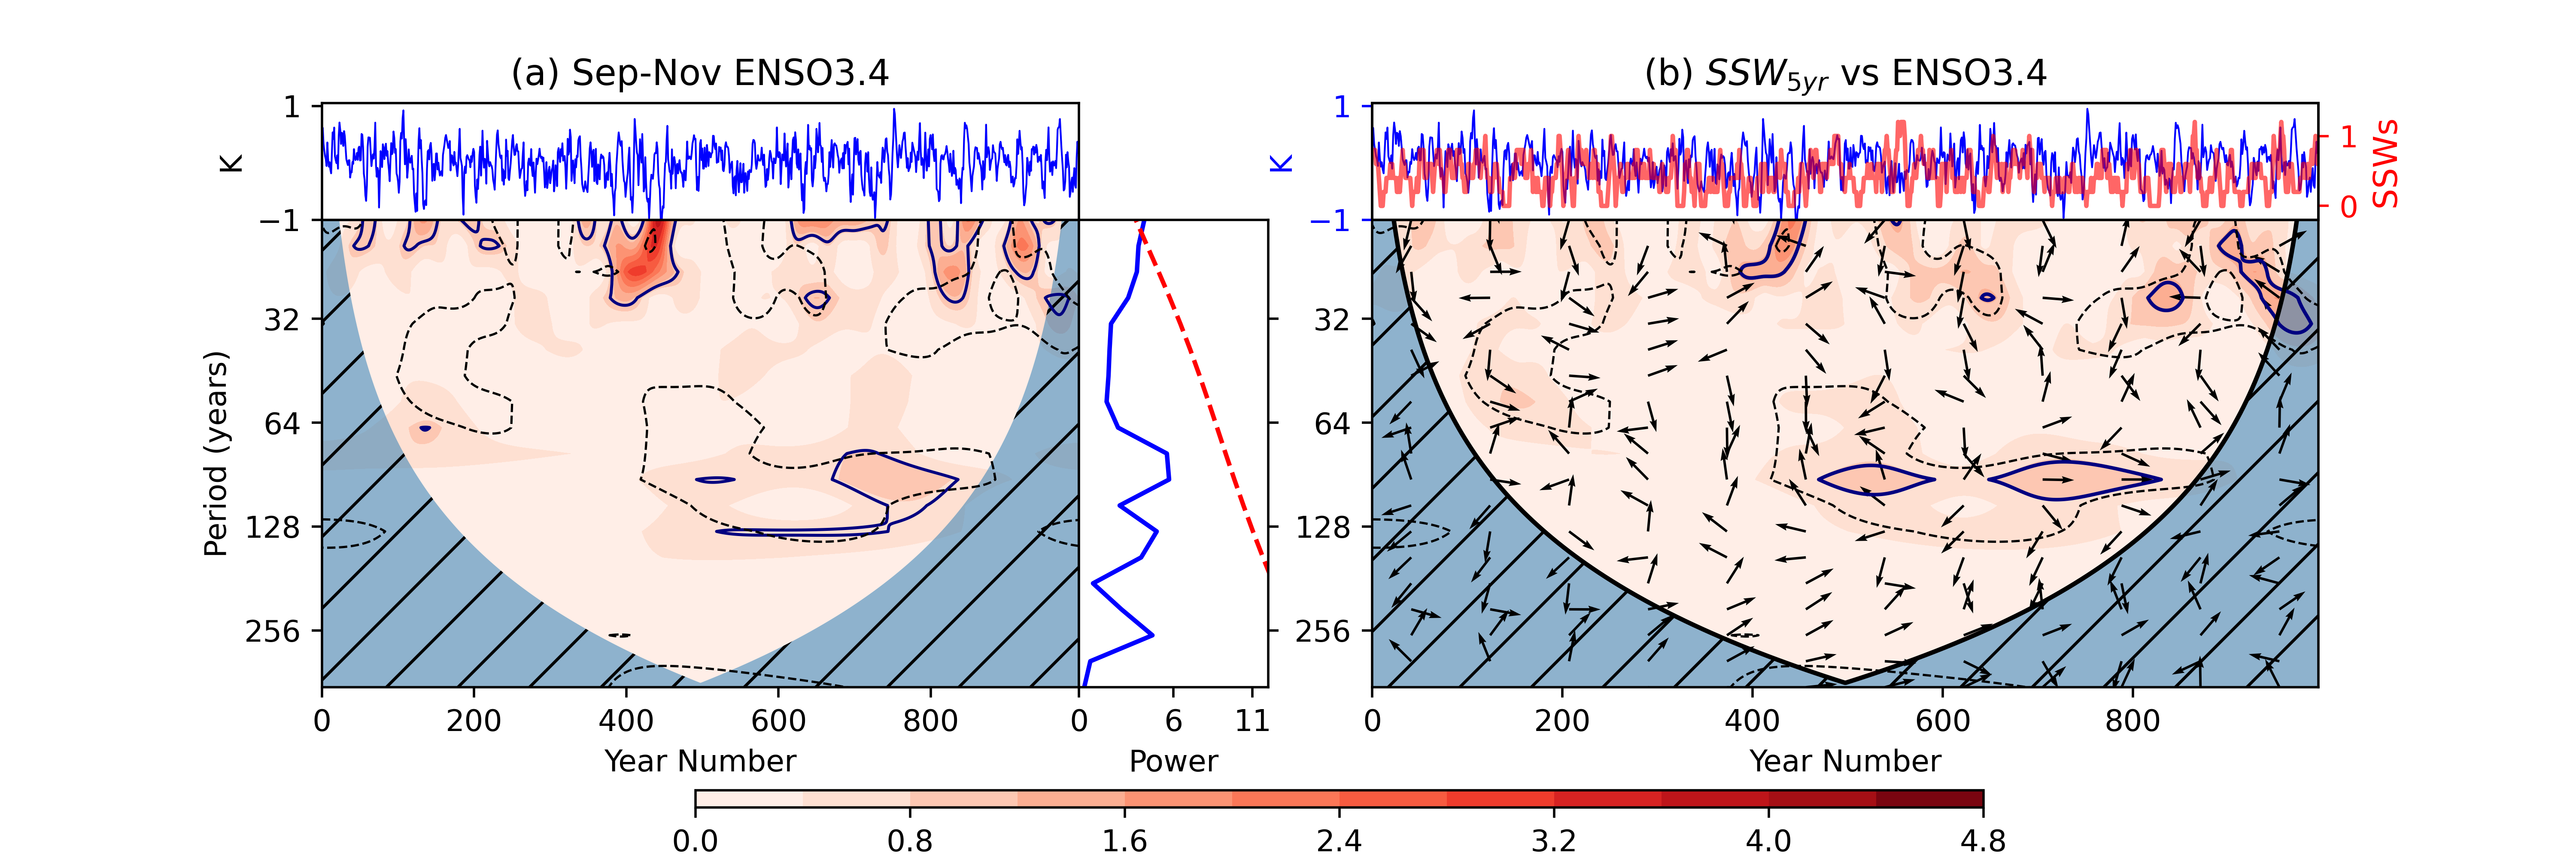
\includegraphics[width = \linewidth]{Figures/Figures-origins/ENSO_wavelet_combined.png}
\caption[Wavelet power spectrum for Sep-Nov Ni\~{n}o3.4 index and cross power spectrum with SSW$_{5yr}$]{\textbf{(a, top)}: Ni\~{n}o3.4 time series, \textbf{a, bottom left}: Wavelet power spectrum (shaded contours represent wavelet power and navy contours the 95\% significance level compared to an AR1 process), \textbf{a, bottom right}: global wavelet power spectrum (blue) and 95\% confidence level (dashed red). \textbf{b}: Cross spectra between $SSW_5yr$ and the Ni\~{n}o3.4 index. \textbf{b, top}: Ni\~{n}o3.4 and $SSW_5yr$ time series. \textbf{b, bottom}: Cross power spectrum. Shading indicates cross power, navy contours the 95\% confidence interval and arrows the relative phase angle between signals in the time series (to the right: in phase, vertically upwards: $\frac{\pi}{2}$ out of phase with SSWs leading, to the left: $\pi$ out of phase, vertically downwards: $\frac{\pi}{2}$ out of phase Ni\~{n}o3.4 leading). Black, dashed contours on both spectra represent the 95\% confidence intervals for the wavelet power spectrum of $SSW_{5yr}$.}
\label{fig:ENSO_wavelet}
\end{center}
\end{figure}

\begin{figure}[h!]
\begin{center}
\noindent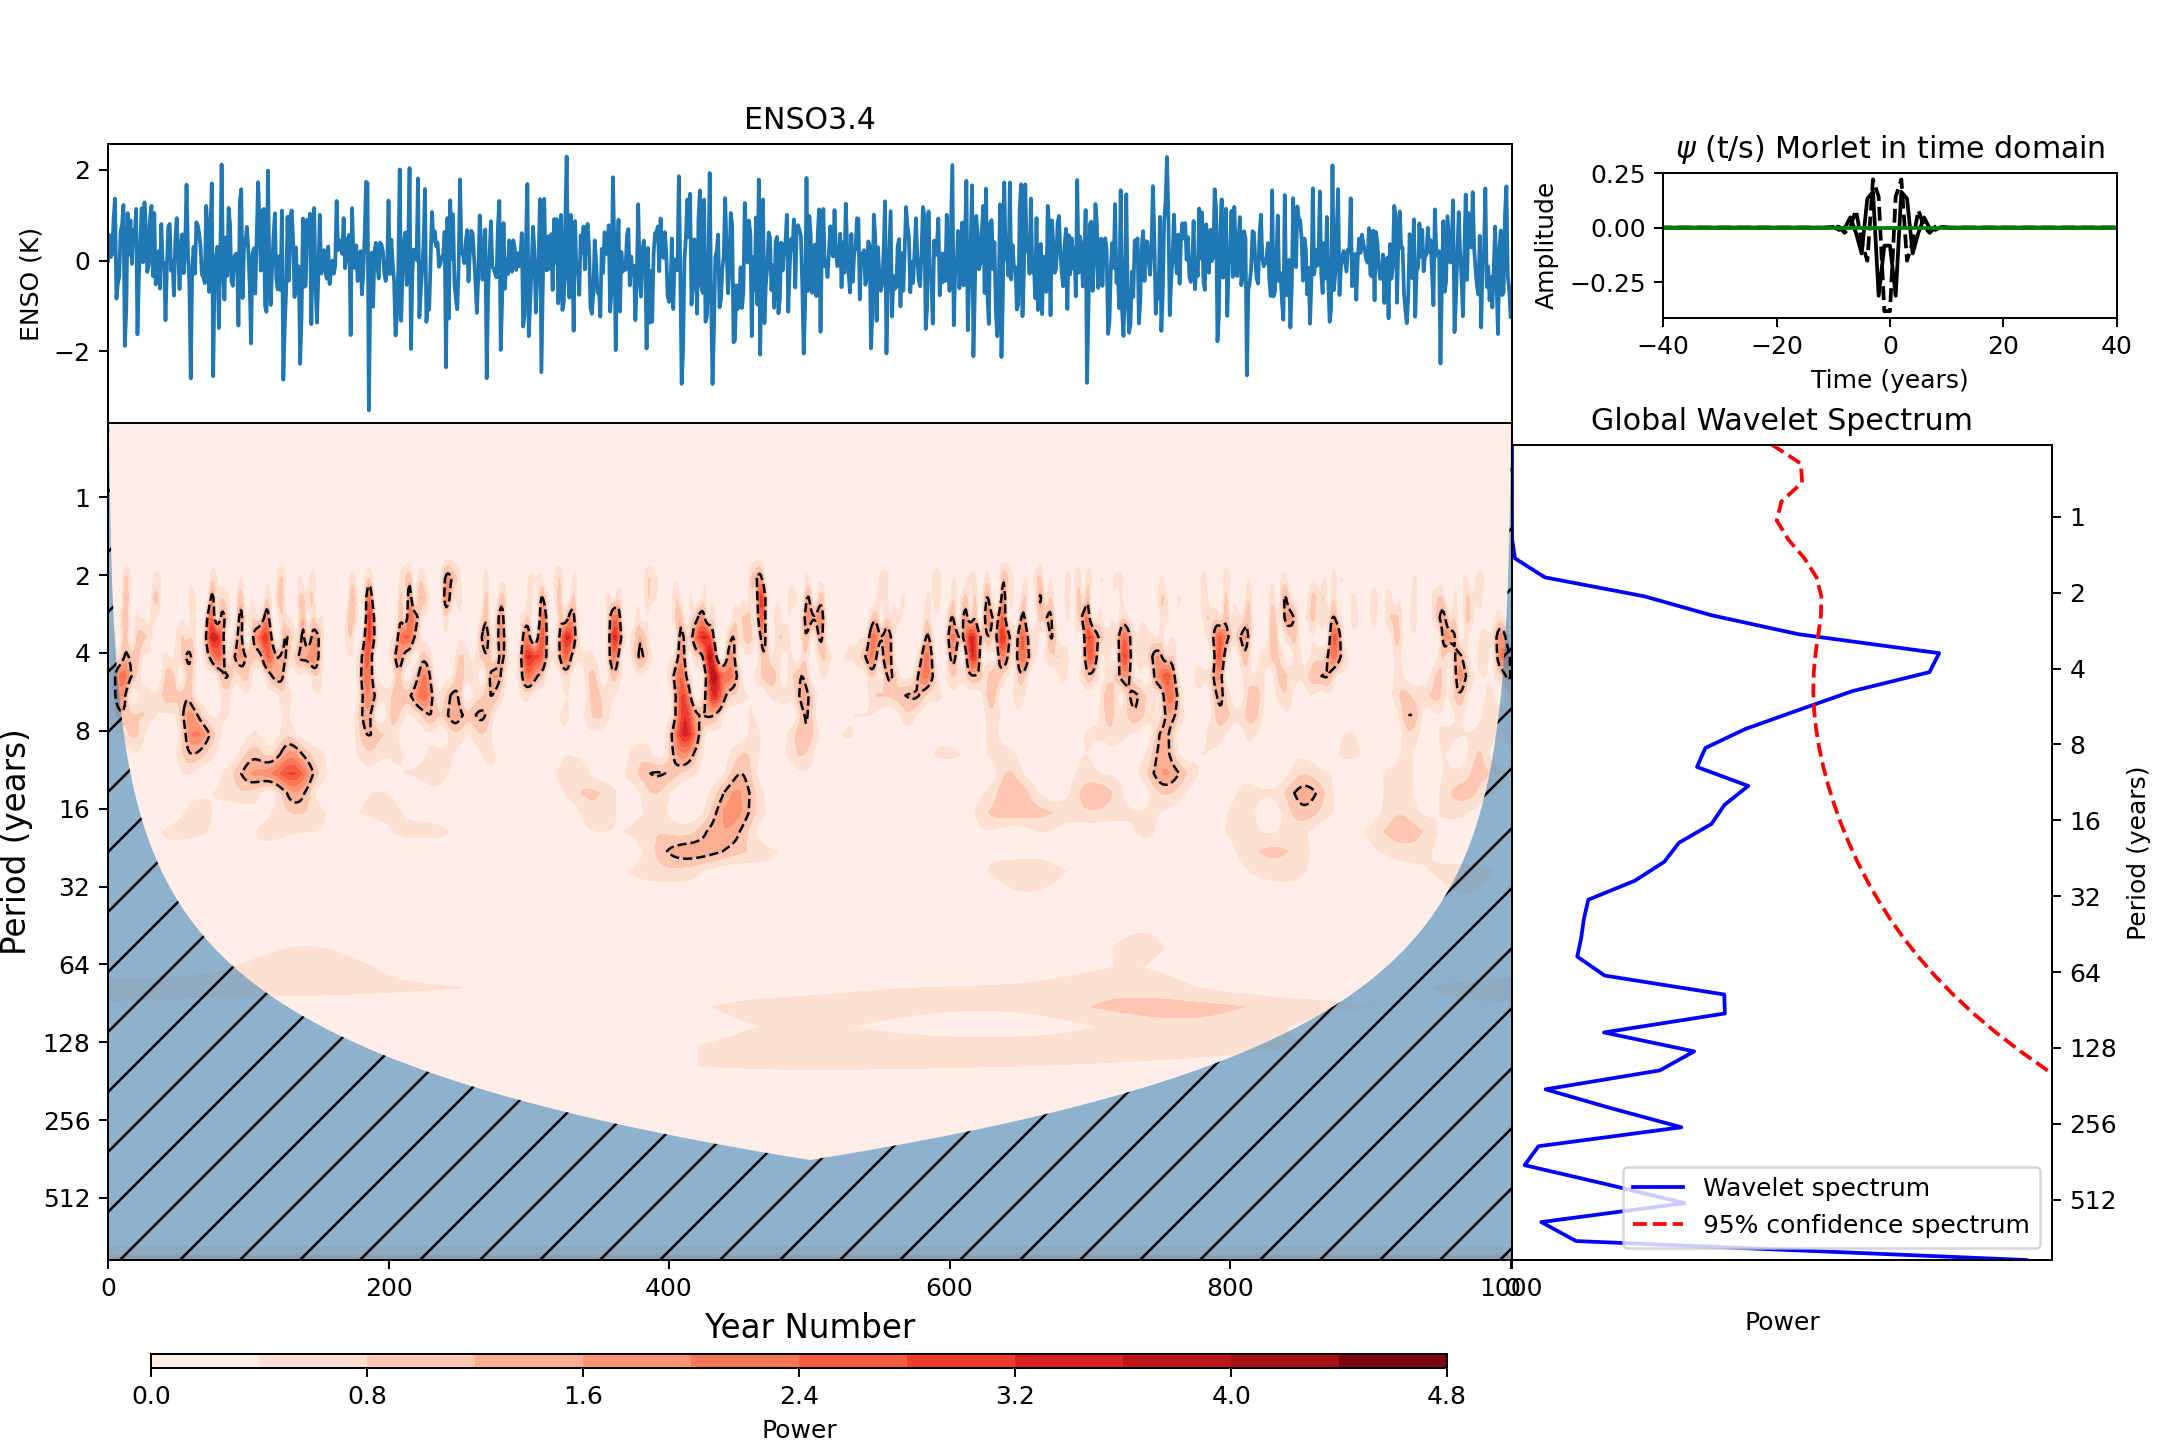
\includegraphics[width = \linewidth]{Figures/Figures-origins/ENSO_wavelet_unsmoothed.png}
\caption{Like figure \ref{fig:SSW_series_wavelet} for the Sep-Nov  Ni\~{n}o3.4 index} 
\label{fig:ENSO_unsmoothed_wavelet}
\end{center}
\end{figure}

In the interest of completeness, we also explore the long-term variability of other tropical ocean regions and their potential teleconnections with the polar vortex. Four additional tropical regions were selected based on those identified by \cite{scaifeTropical2017b} and outlined in section \ref{sec:model_diagnostics}. While all four regions show some elements of multi-decadal variability (figure \ref{fig:tropical_SST_wavelet}), particularly the Tropical Atlantic with a peak period of approximately 140 years for 700 years of the simulation, none of the spectra show variability that coincides well with that of $SSW_{5yr}$. There is some overlap of the Atlantic and Tropical East Pacific spectra with the regions of significant periodicity at around 60-90 years in the $SSW_{5yr}$ spectrum but, like the Ni\~{n}o3.4 index, the overlaps between the series are minimal and cannot reasonably explain the vortex signal, especially the signal of period approximately 90 years that persists in $SSW_{5yr}$ for around 450 years (figure \ref{fig:tropical_SST_wavelet} dashed contours).

\begin{figure}[h!]
\begin{center}
\noindent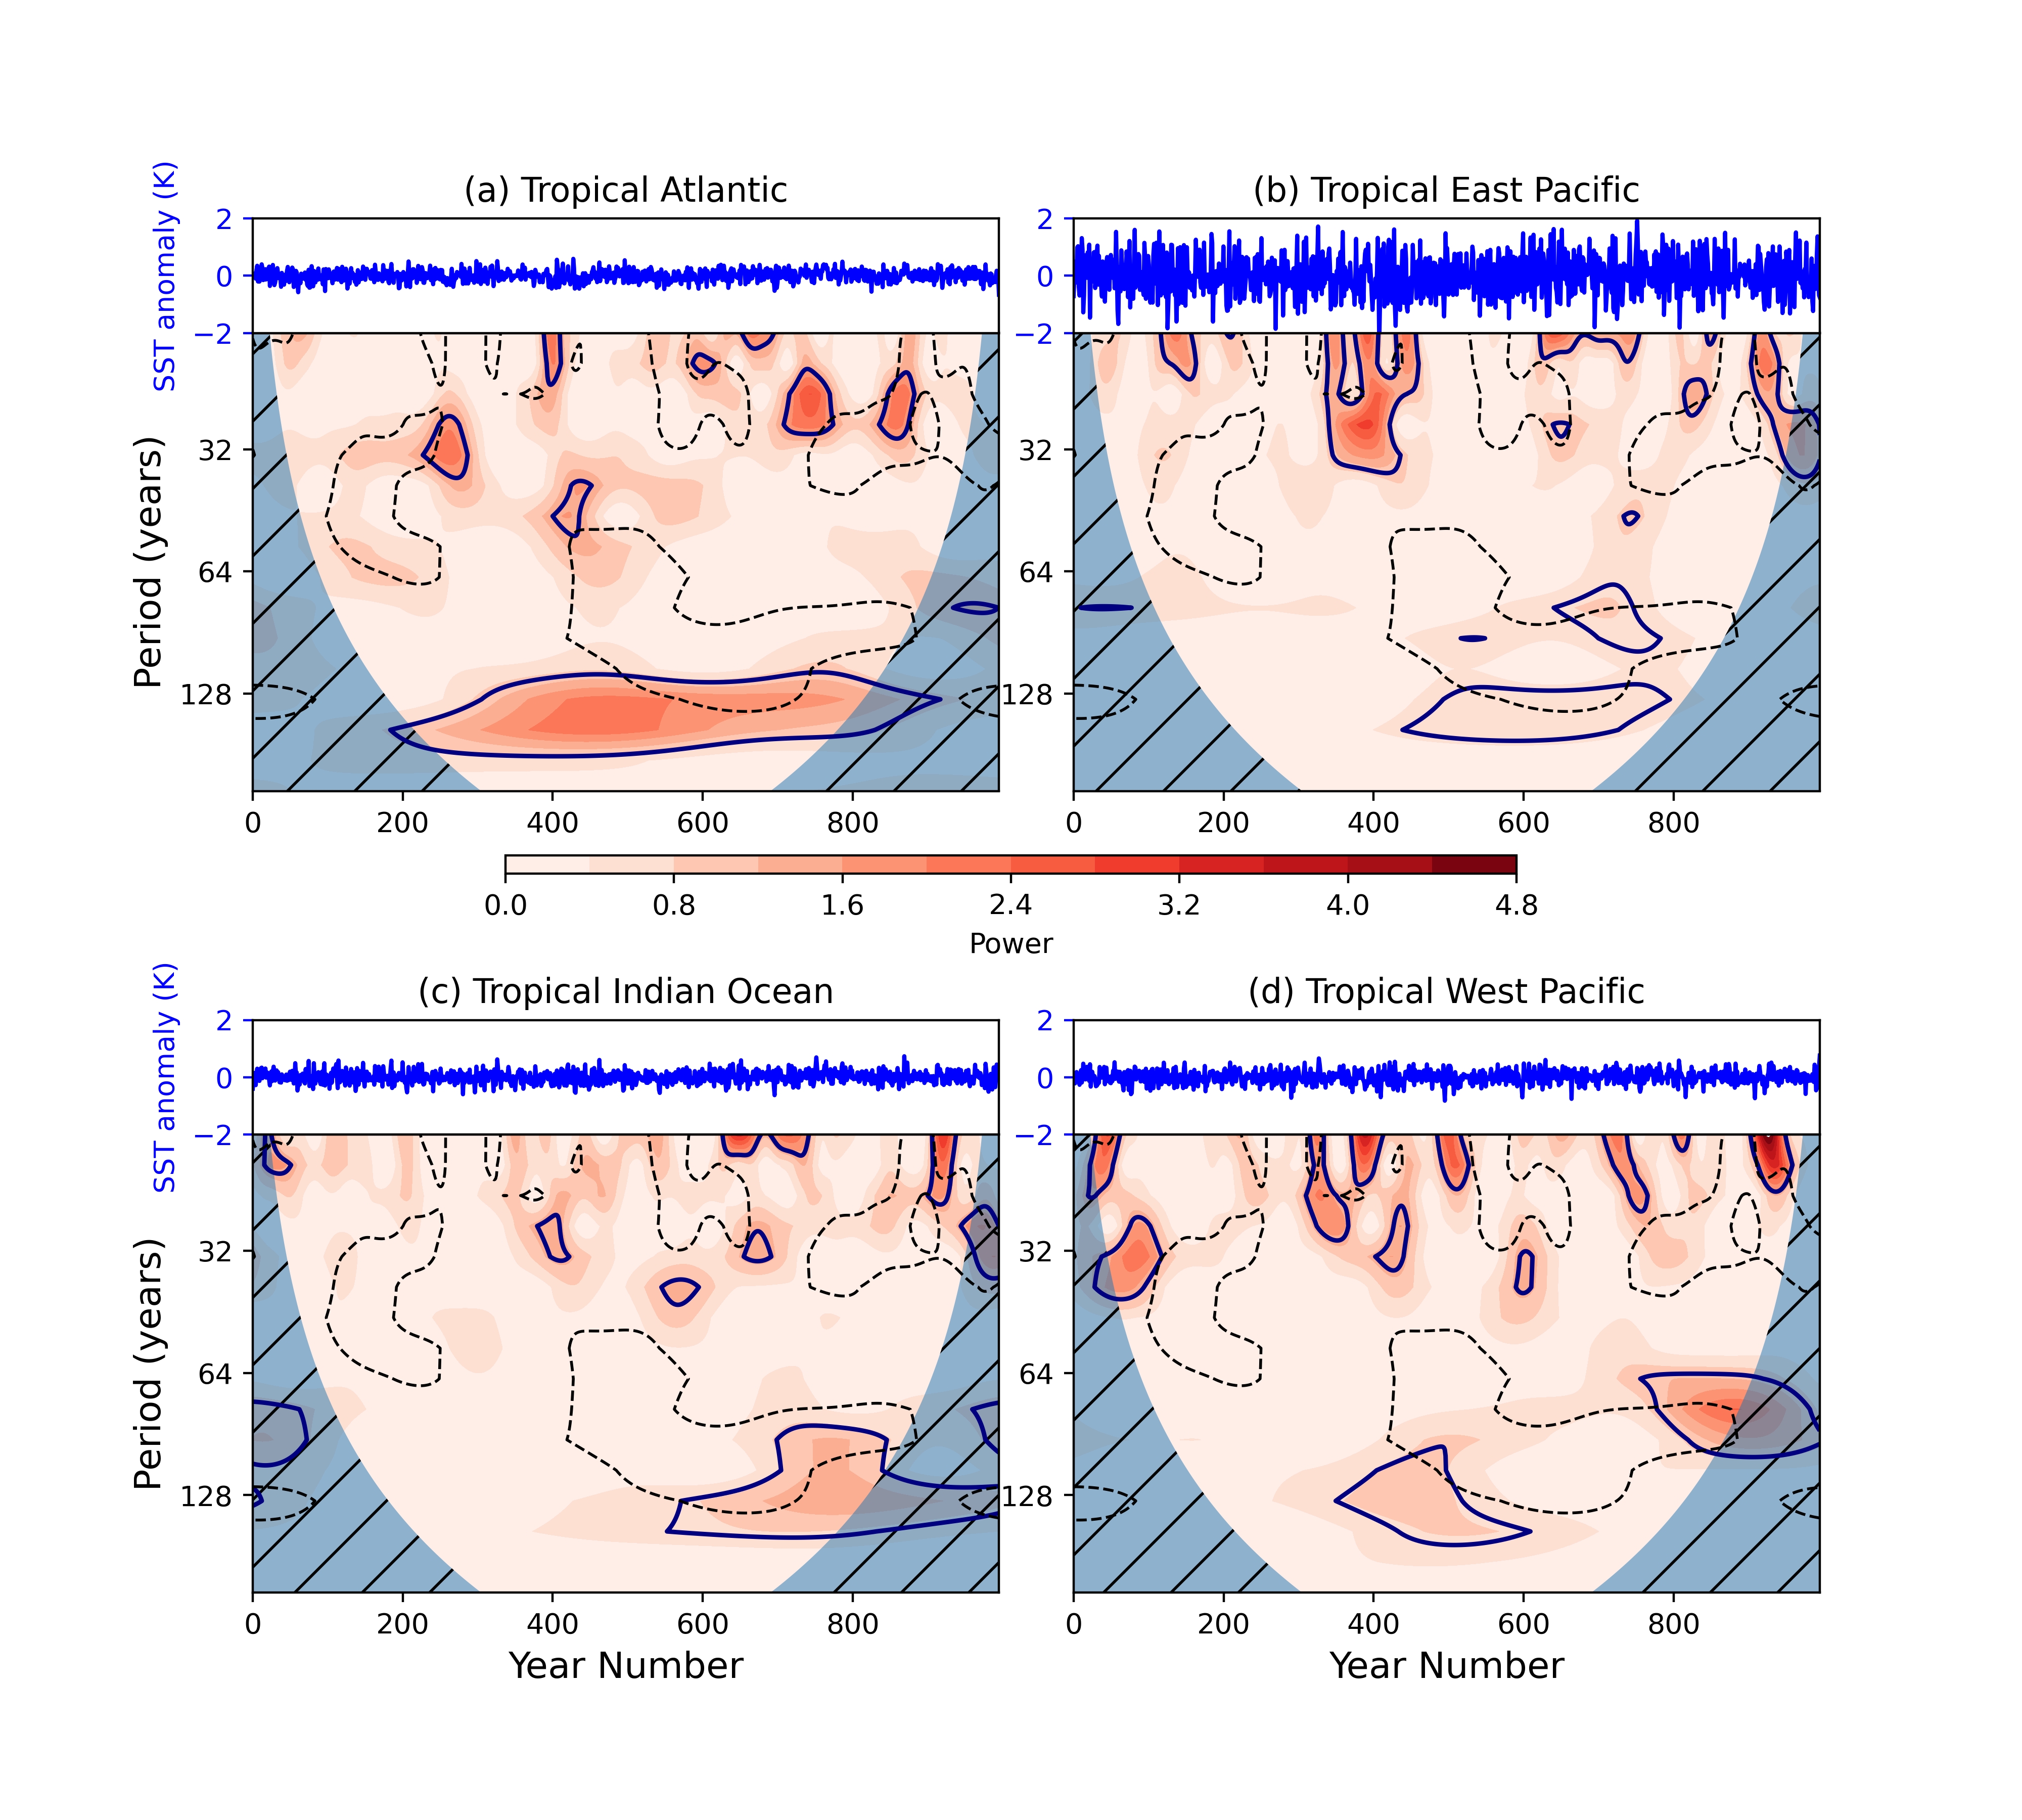
\includegraphics[width = 0.8\linewidth]{Figures/Figures-origins/SSTs_tropical_wavelet.png}
\caption{Sep-Nov SST anomaly time series and associated wavelet power spectrum for Tropical Atlantic (5$^{\circ}$\,S–5$^{\circ}$\,N, 60$^{\circ}$\,W–0$^{\circ}$\,W), Tropical East Pacific (5$^{\circ}$\,S–1$^{\circ}$\,N, 160$^{\circ}$\,E–270$^{\circ}$\,E), Tropical West Pacific (5$^{\circ}$\,S–25$^{\circ}$\,N, 110$^{\circ}$\,E–140$^{\circ}$\,E) and Tropical Indian Ocean (5$^{\circ}$\,S–10$^{\circ}$\,N, 45$^{\circ}$\,E–100$^{\circ}$\,E). Shading indicates wavelet power, yellow contours show the 95\% confidence level when the power is compared to and AR1 red-noise process and dashed contours indicate the 95\% confidence level for the power spectrum of $SSW_5yr$.}
\label{fig:tropical_SST_wavelet}
\end{center}
\end{figure}

The strength of the Aleutian Low (AL) has also been used as an indicator of tropospheric wave forcing and its influence on the polar vortex \citep{wooConnection2015b}. We perform a similar wavelet and cross-spectrum analysis using an index based on the strength of the modelled NH winter (Dec-Mar) AL (see section \ref{sec:model_diagnostics} for details). The wavelet power spectrum for the 5-year smoothed AL index (figure \ref{fig:AL_wavelet}a) exhibits elements of periodic signals with maximum power corresponding to a period of around 55 years (between 40-60 years) but with fairly minimal overlap with the regions enclosed by the 95\% confidence level in the corresponding SSW wavelet analysis (green contours). AL indices derived from different winter months give similar spectral patterns (not shown).  The cross spectrum analysis between the AL and $SSW_5yr$ (figure \ref{fig:AL_wavelet}b) highlights this relatively small region of overlap in the interval between years 400-500. However, the phase relationship, indicated by the arrows in that region of overlap is difficult to interpret. The proposed physical mechanism of coupling between the AL and the vortex \citep{wooConnection2015b} involves an association between a deeper AL (i.e. lower pressure and hence a negative anomaly) with increased frequency of SSWs. This negative correlation would give rise to arrows pointing to the left if the relationship was present. In contrast, the upward arrows in figure 9b indicate a $\frac{\pi}{2}$ phase difference between the indices on these 60 year timescales, suggesting that peaks in $SSW_{5yr}$ variations are associated with maximum rates of change of the AL index at the same periods. As with Ni\~{n}o3.4, the spectra of the AL shares some features with that of the PDO (figure \ref{fig:PDO_wavelet}). This is consistent with studies into these modes of variability which find significant correlation of the PDO and AL \citep{mantuaPacific1997a, rodionovSpatial2005b} as well as studies that examine influence of PDO on vortex strength through a pathway involving the AL and ENSO \citep{raoModulation2019d}. Despite this possible pathway, the relatively short time interval of overlap between the AL and $SSW_{5yr}$ signals at the 60-yr period, the absence of any significant signal around the 90-yr period, together with the inconsistent phase relationships, points to a conclusion that AL forcing is unlikely to be the primary driver of long-term variability in $SSW_{5yr}$. Indeed, examination of the cross-spectrum between the un-smoothed AL and SSW indices (figure \ref{fig:AL_unsmoothed_wavelet}) shows little indication of a coherent relationship between periodic signals in the two indices at any timescale. Finally, while the regression results of the un-smoothed indices give a significant coefficient for the AL (table 1), its magnitude is small compared to that of Ni\~{n}o3.4 and the deep QBO, the uncertainty on the coefficient is large and the associated p value is close to the 95\% significance boundary. The weak relationship between the AL and SSWs is unexpected due to the well acknowledged influence of the AL over planetary wave flux in the upper troposphere \citep{wooConnection2015b}. To attempt to address this, we also analyse an AL metric evaluated as the area weighted average over a box recommended by \cite{garfinkelWhy2012b} who use an SSW precursor region in 500hPa height defined by $52.5^{\circ}$–$72.5^{\circ}N$, $165^{\circ}$–$195^{\circ}E$. However, we find a lower correlation between this measure and our SSW timeseries than between the original EOF based metric and SSWs ($r = -0.21$ for the EOF based AL and $r = -0.13$ for the box based AL).

%---------------------------------------------------------------

\begin{figure}[h!]
\begin{center}
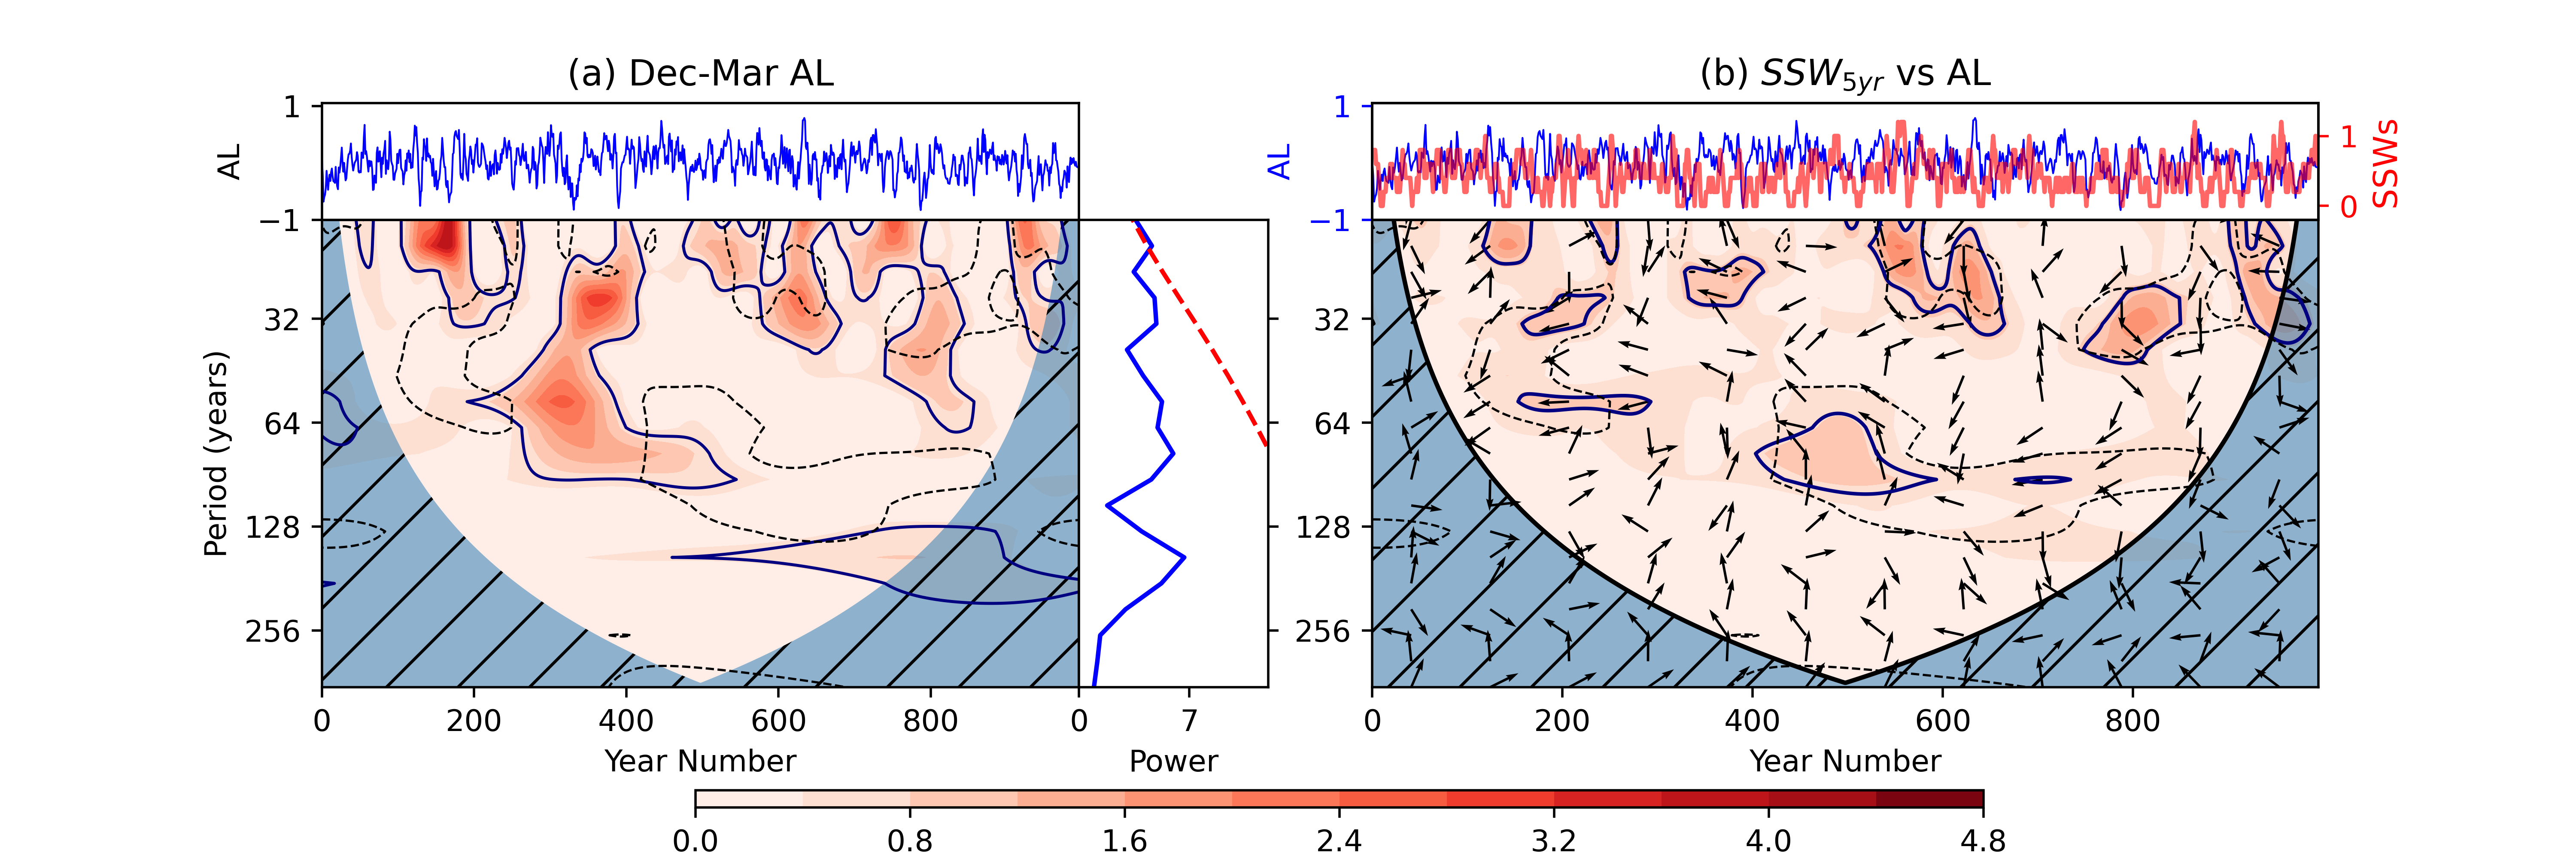
\includegraphics[width = \linewidth]{Figures/Figures-origins/AL_wavelet_combined.png}
\caption{Like figure \ref{fig:ENSO_wavelet} for the Dec-Mar Aleutian Low index smoothed with a 5 year window. \textbf{a}: AL time series and associated wavelet power spectrum. \textbf{b}: Cross power spectrum between AL and $SSW_{5yr}$.}
\label{fig:AL_wavelet}
\end{center}
\end{figure}

\begin{figure}[h!]
\begin{center}
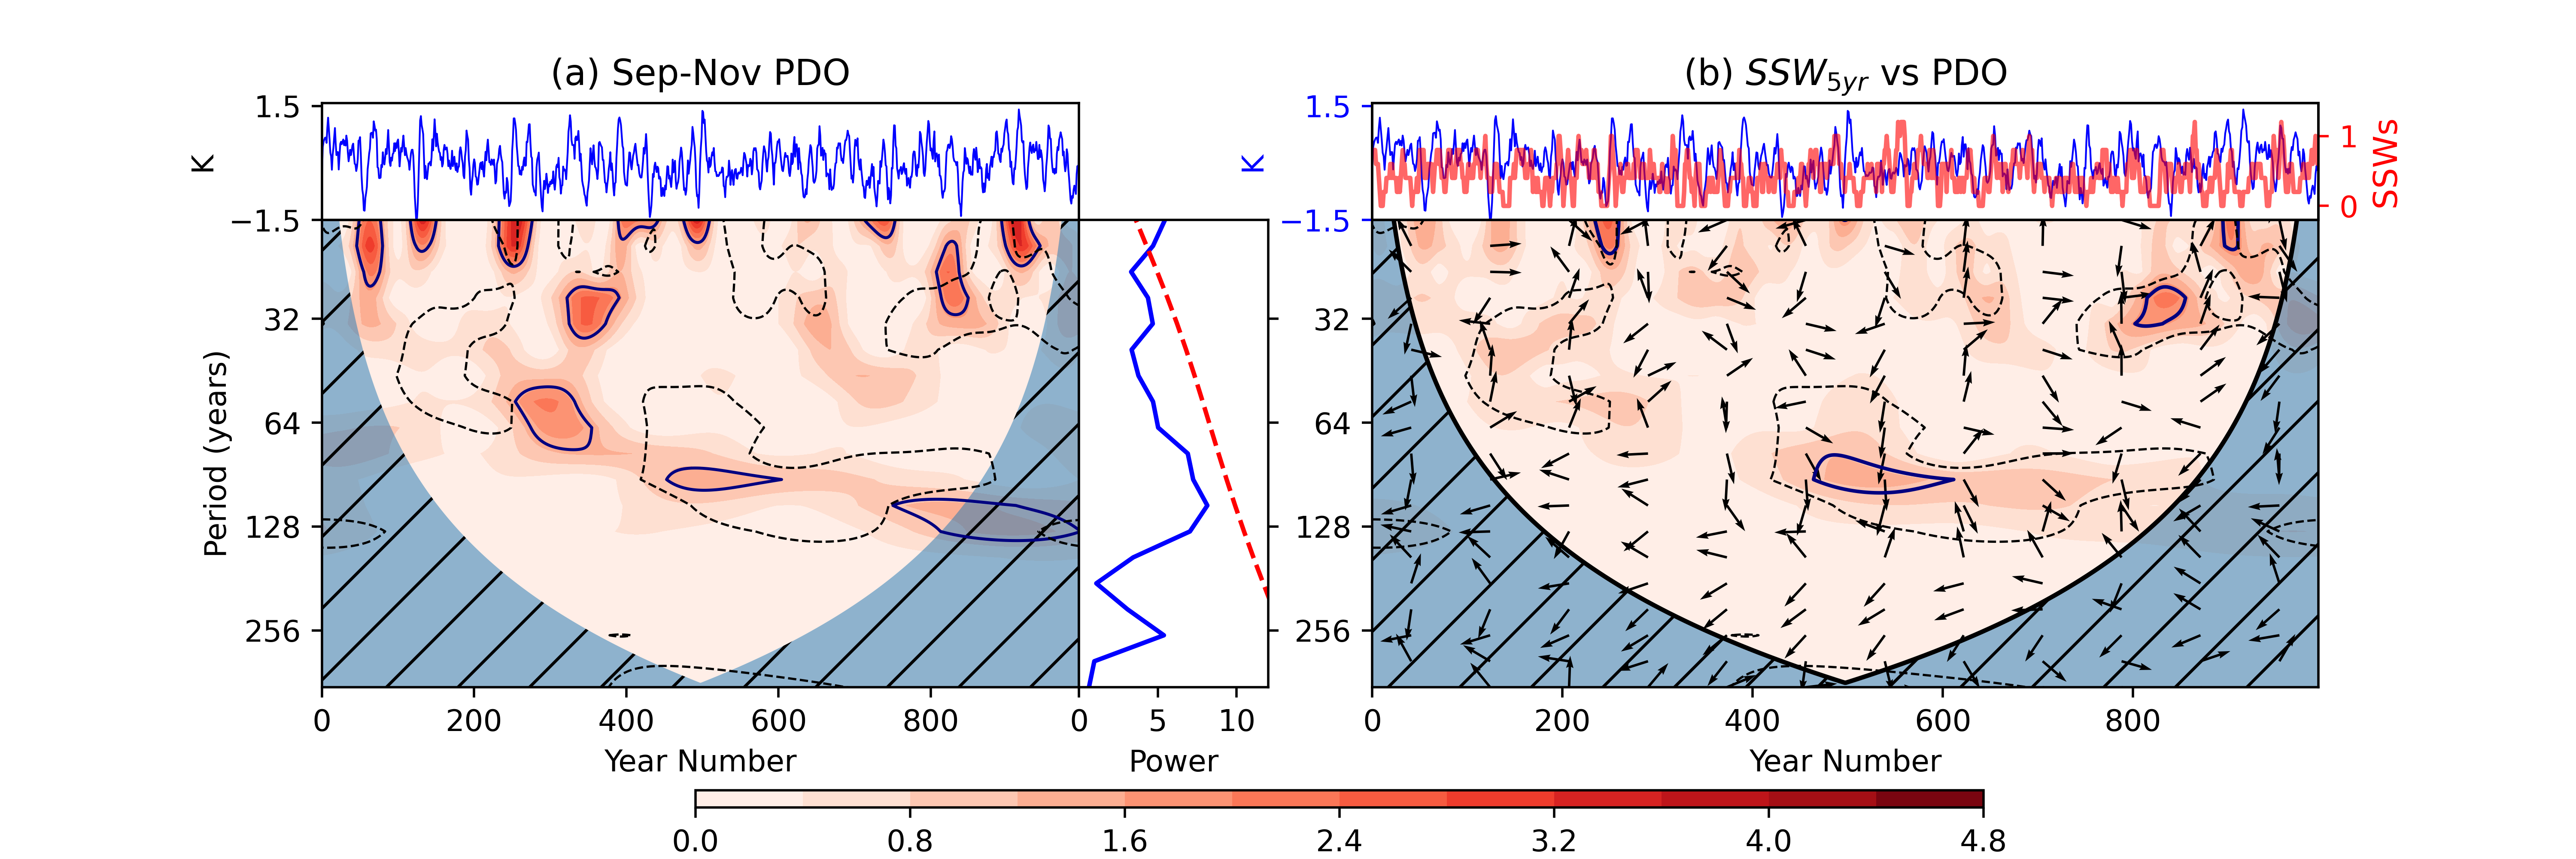
\includegraphics[width = \linewidth]{Figures/Figures-origins/PDO_wavelet_combined.png}
\caption[Wavelet power spectrum for 5 year mean PDO index from UKESM]{Like figure \ref{fig:ENSO_wavelet} for the Sep-Nov PDO index smoothed with a 5 year window. \textbf{a}: PDO time series and associated wavelet power spectrum. \textbf{b}: Cross power spectrum between PDO and $SSW_{5yr}$.}
\label{fig:PDO_wavelet}
\end{center}
\end{figure}

\begin{figure}[h!]
\begin{center}
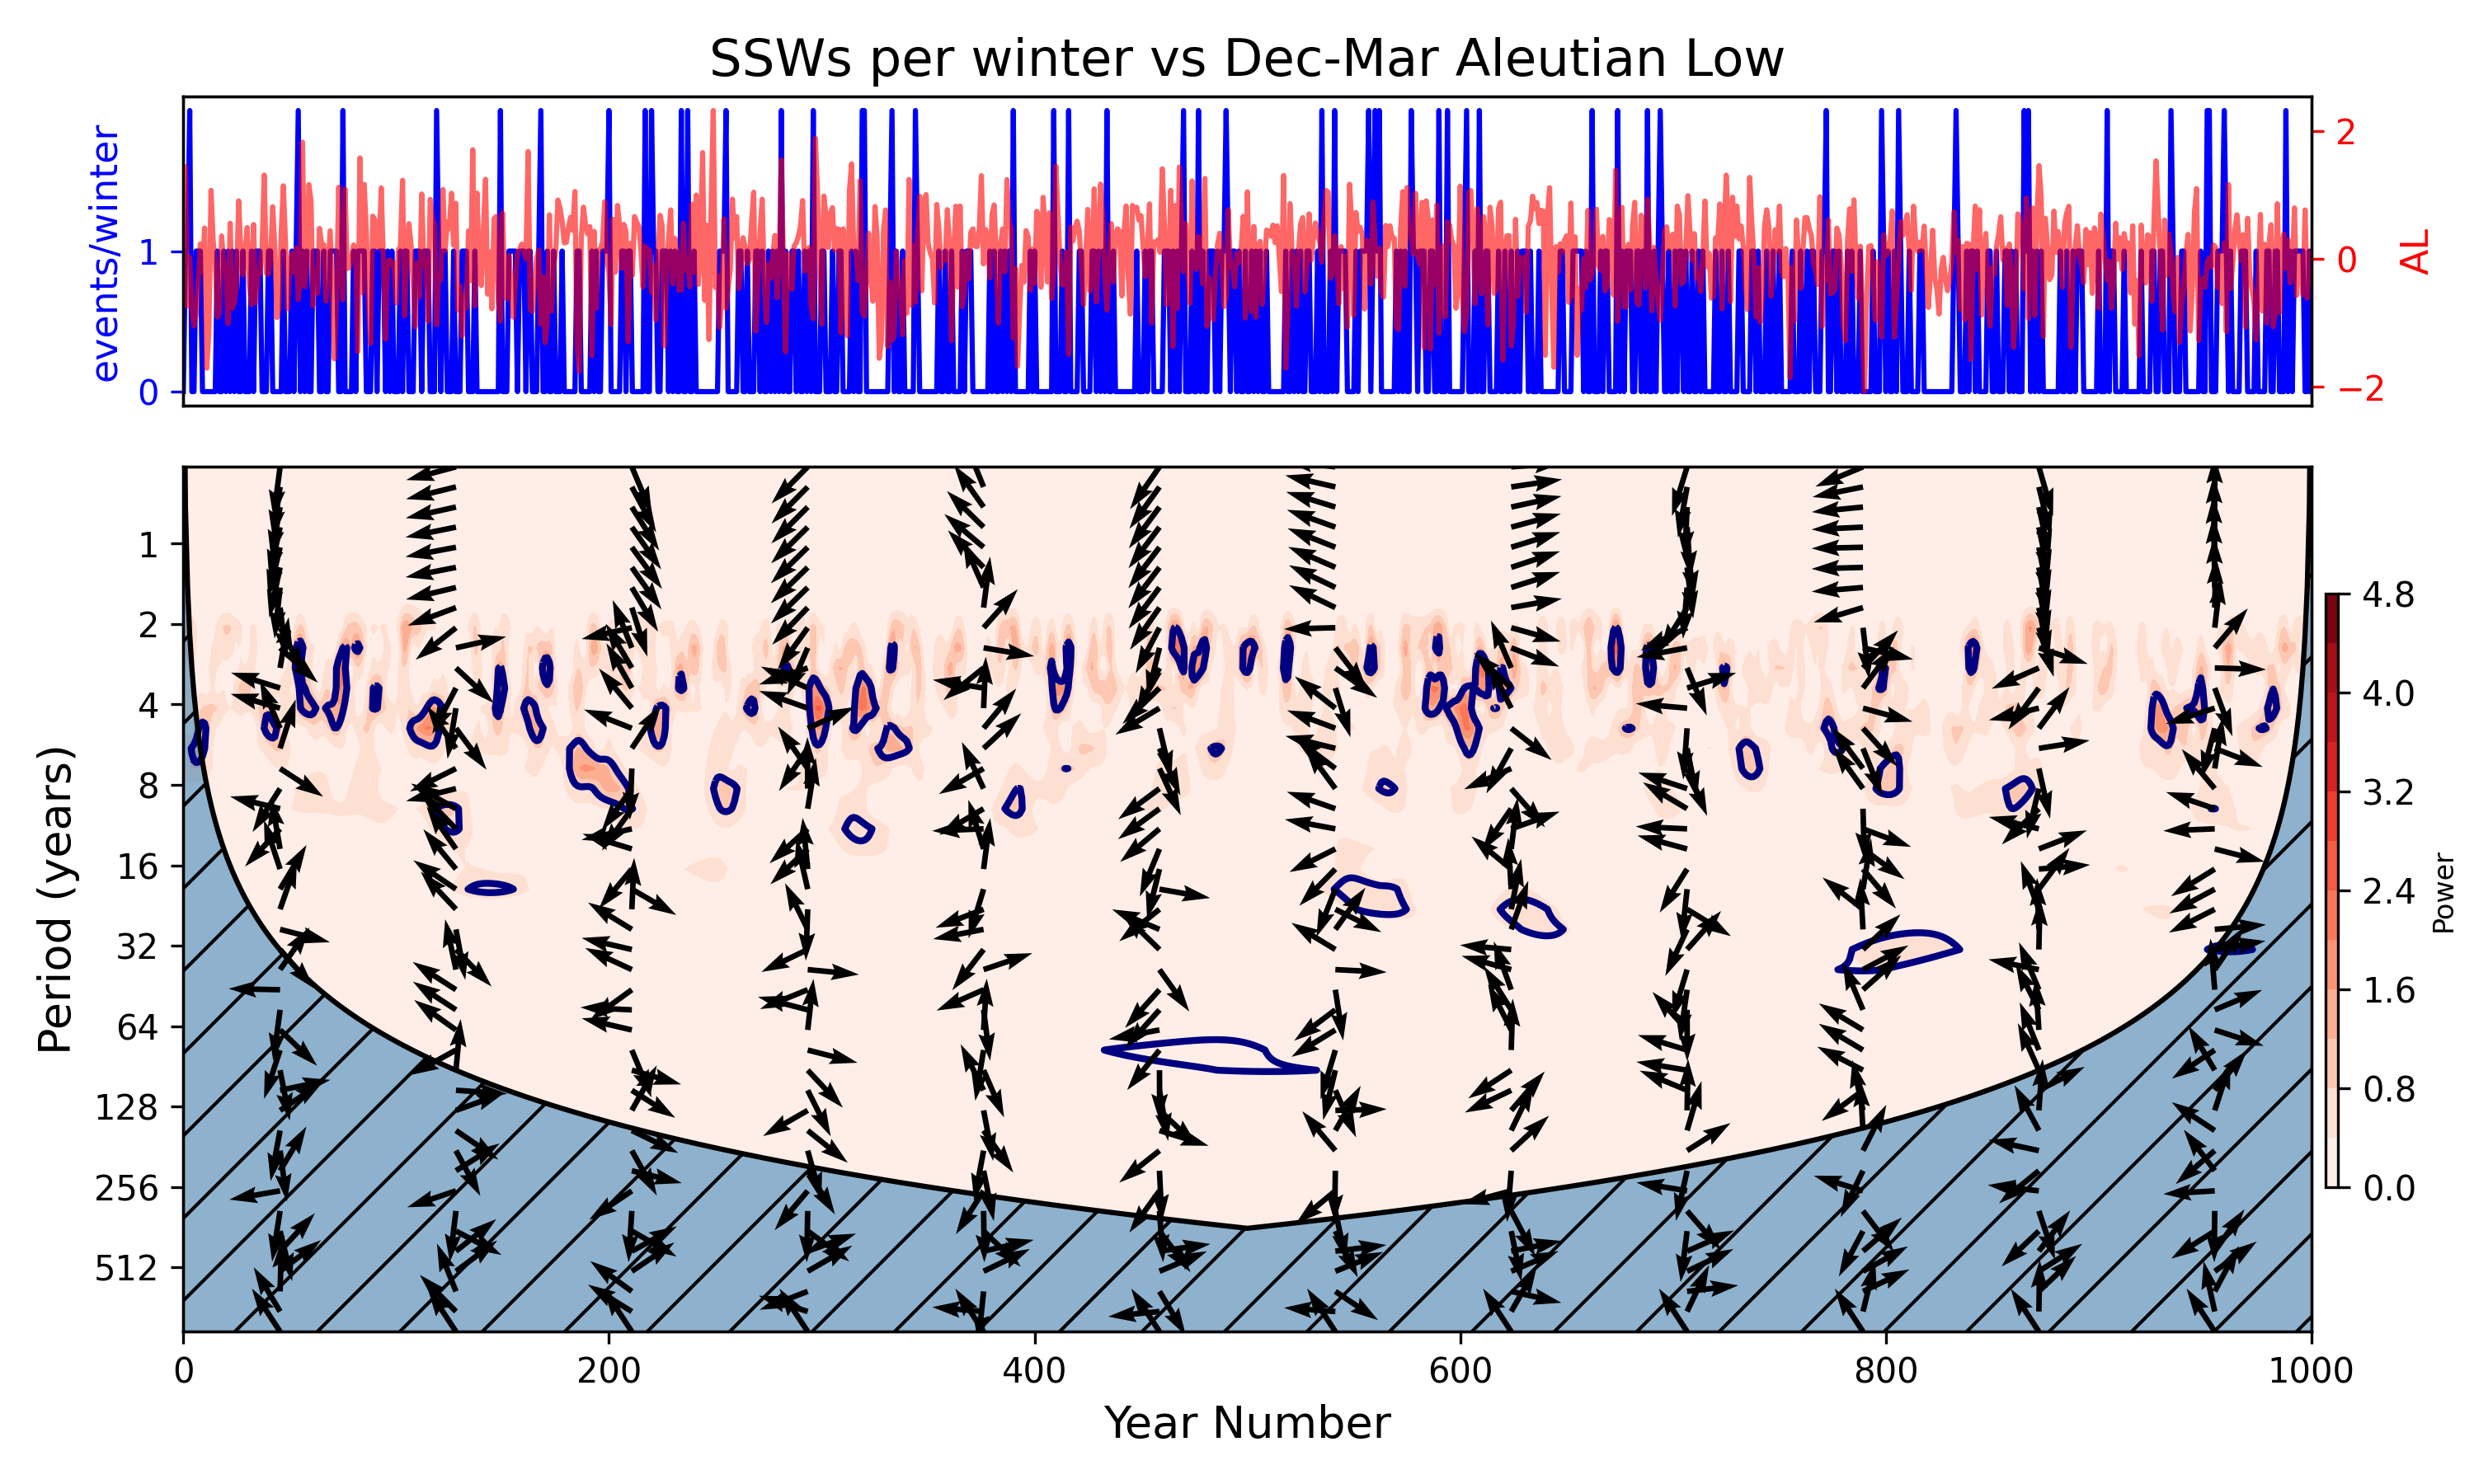
\includegraphics[width = \linewidth]{Figures/Figures-origins/SSWs_vs_AL_wavelet_unsmoothed.png}
\caption[Wavelet cross power spectrum between AL index and SSW timeseries]{\textbf{Top}: December–March Aleutian Low index (red) and SSWs per NH winter (blue) time series. \textbf{Bottom} Cross-wavelet power spectrum between the two time series.}
\label{fig:AL_unsmoothed_wavelet}
\end{center}
\end{figure}

%---------------------------------------------------------------

\section{Vortex-QBO Interactions}
Despite some coincident signals between tropical SSTs, AL and $SSW_{5yr}$, long-term variability in these surface indices are unable to fully account for the  multidecadal signals in SSW frequency. An additional potential source of internally generated long-term variability may reside within the stratosphere. Studies have noted relatively long-term variations in the strength of the Holton-Tan relationship \citep{luDecadalscale2008,luMechanisms2014c,ospreyClimatology2010b} although the cause of these variations is not well understood. In order to investigate this figure \ref{fig:QBO_levs} shows the wavelet power spectrum of early winter (Sep-Nov) QBO winds evaluated at selected levels. Since the QBO evolves relatively slowly, employing Sep-Nov averaged winds provides a reasonable representation of the QBO and also allows us to evaluate the in-season lagged relationship between the QBO and subsequent occurrence of an SSW. There is a clear signal between 2 and 4 years for the majority of the simulation, as expected, but no prominent power at longer periods,  confirming that there is no significant long-term variability in the periodicity of the QBO winds that could explain the long-term variations in $SSW_{5yr}$ via the Holton-Tan relationship.

\begin{center}
\begin{figure}[h!]
\noindent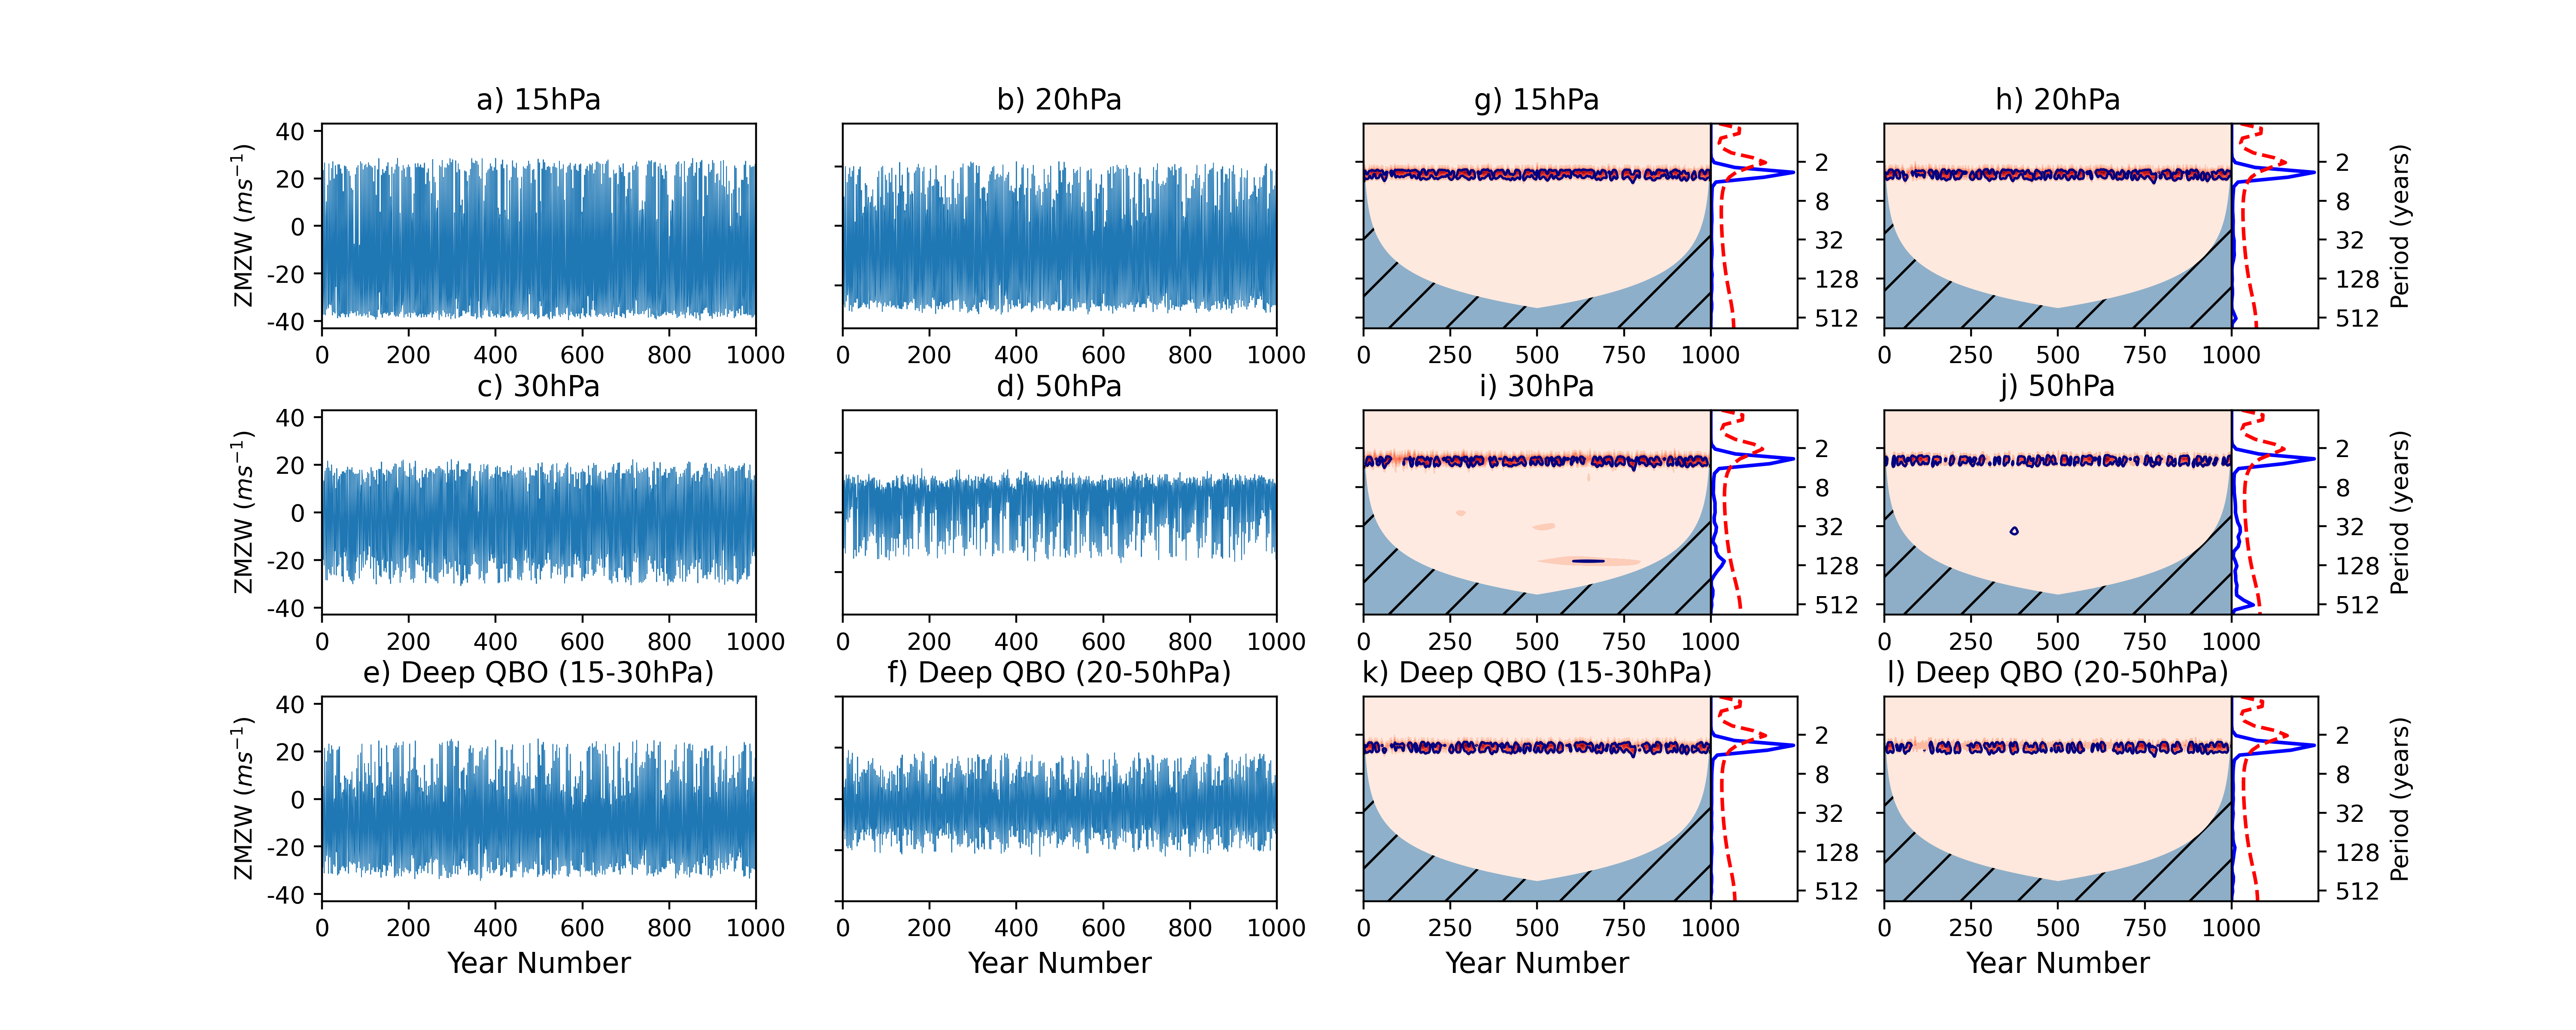
\includegraphics[width = \linewidth]{Figures/Figures-origins/QBO_levels.png}
\caption[QBO timeseries and associated wavelet power spectra at different levels in UKESM]{\textbf{(a-f)}: Sep-Nov mean ZMZW averaged between 5$^\circ$S--5$^\circ$N latitude on different pressure levels (a-e) and the deep metric averaged between 15--30\,hPa (f). \textbf{(g-l)}: Wavelet power spectra for each time series shown in (a-c). Shading represents wavelet power with a colour scale the same as that seen in figure \ref{fig:SSW_series_5yr_wavelet} and navy contours indicate regions of significant power (>95\% confidence interval) compared to a background AR1 process.}
\label{fig:QBO_levs}
\end{figure}
\end{center}

%---------------------------------------------------------------

While the wavelet analysis technique is able to isolate and reveal frequency modulations very well it is less suited to examine amplitude modulations which are clearly evident by eye in some of the QBO index time-series. For example, both the 20 hPa and deep (15-30 hPa) QBO time series show multi-decadal variations in the magnitude of the westerly phase while the easterly phase amplitudes are relatively uniform in time. Similarly, the 50\,hPa and 30\,hPa time series show amplitude modulation predominantly in the easterly phase. This amplitude modulation can be highlighted by taking the Hilbert Transform of each QBO time-series (figure \ref{fig:QBO_levs_amp}a-f). Wavelet analysis of the transformed QBO time series now shows significant power on multidecadal timescales (figure \ref{fig:QBO_levs_amp}g-l). In particular, the 20\,hPa and deep QBO time-series exhibit signals coincident in time and around similar periods (60-90 years) to those observed in $SSW_5yr$. On the other hand, the QBO indices based on equatorial winds at 50\,hPa or 30\,hPa show minimal power at these periods, despite showing a strong intraseasonal HT relationship (figure \ref{fig:holton_tan_comp}). Given that the 15-30 hPa deep QBO  index exhibits  both multidecadal timescale variability and a strong intraseasonal HT coupling, we continue further analysis of the SSW-QBO interactions using the 15-30 hPa index. 

%---------------------------------------------------------------

\begin{figure}[h!]
    \begin{center}
    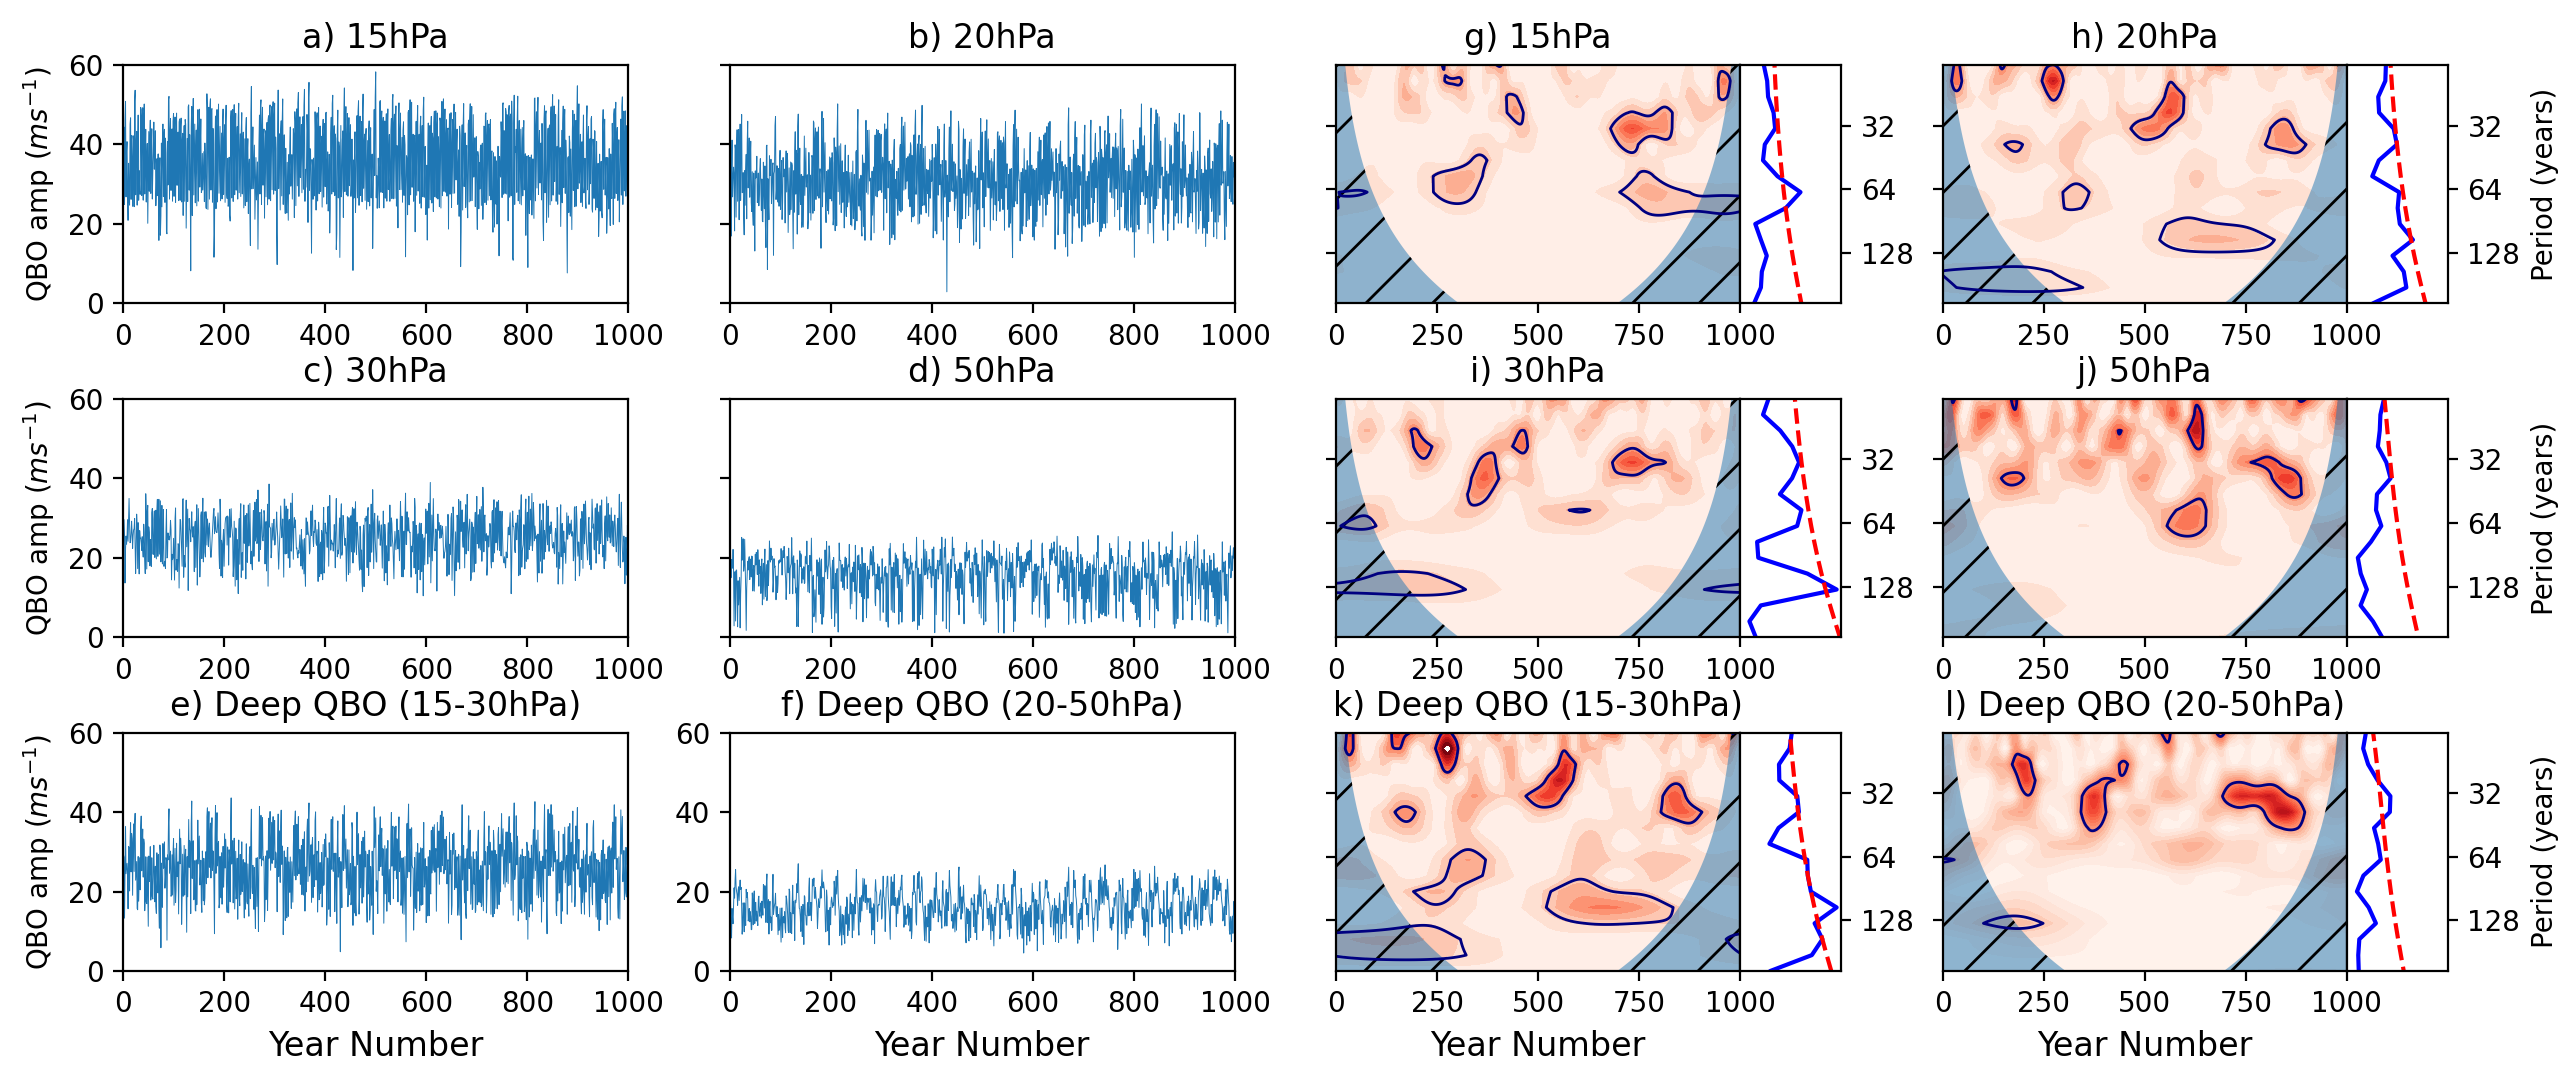
\includegraphics[width = \linewidth]{Figures/Figures-origins/QBO_levels_amp.png}
    \caption[QBO amplitude timeseries and associated wavelet power spectra at different levels in UKESM]{\textbf{(a-e)}: Hilbert amplitude of Sep-Nov mean ZMZW averaged between 5$^\circ$\,S--5$^\circ$\,N latitude on different pressure levels (a-e) and the deep metric averaged between 15--30\,hPa (f). \textbf{(g-l)}: Wavelet power spectra for each time series shown in (a-c). Shading represents wavelet power with a colour scale the same as that seen in figure \ref{fig:SSW_series_5yr_wavelet} and navy contours indicate regions of significant power (>95\% confidence interval) compared to a background AR1 process.}
    \label{fig:QBO_levs_amp}
    \end{center}
\end{figure}

%---------------------------------------------------------------

Wavelet analysis of the 5-year smoothed deep (15-30\,hPa) QBO amplitude modulation index (figure 12a) enhances the clarity of the long-term periodicity, showing statistically significant power at around 90 years in the interval between year numbers 500-800. The cross power between $SSW_5yr$ and this QBO amplitude modulation index (figure \ref{fig:QBO_SSW_subfig}) coincides extremely well with the signals observed in $SSW_5yr$ at around 90 years. There are also coincident features at other timescales, although the feature between years 450-550 at periods of 60 years is less well captured. The phase-relationship arrows in the main region of long-term variability (periods around 90 years in the interval 450-800 years) point broadly to the left ($\pi$ phase shift), indicating that the signals are approximately anti-phased (the slight downward pointing of the arrows suggests a small deviation from this lag-zero relationship and is discussed below). The anti-phase relationship is consistent with the HT relationship in which a westerly (positive) QBO anomaly corresponds to a reduction in the frequency of SSWs.

%---------------------------------------------------------------

\begin{center}
\begin{figure}[h!]
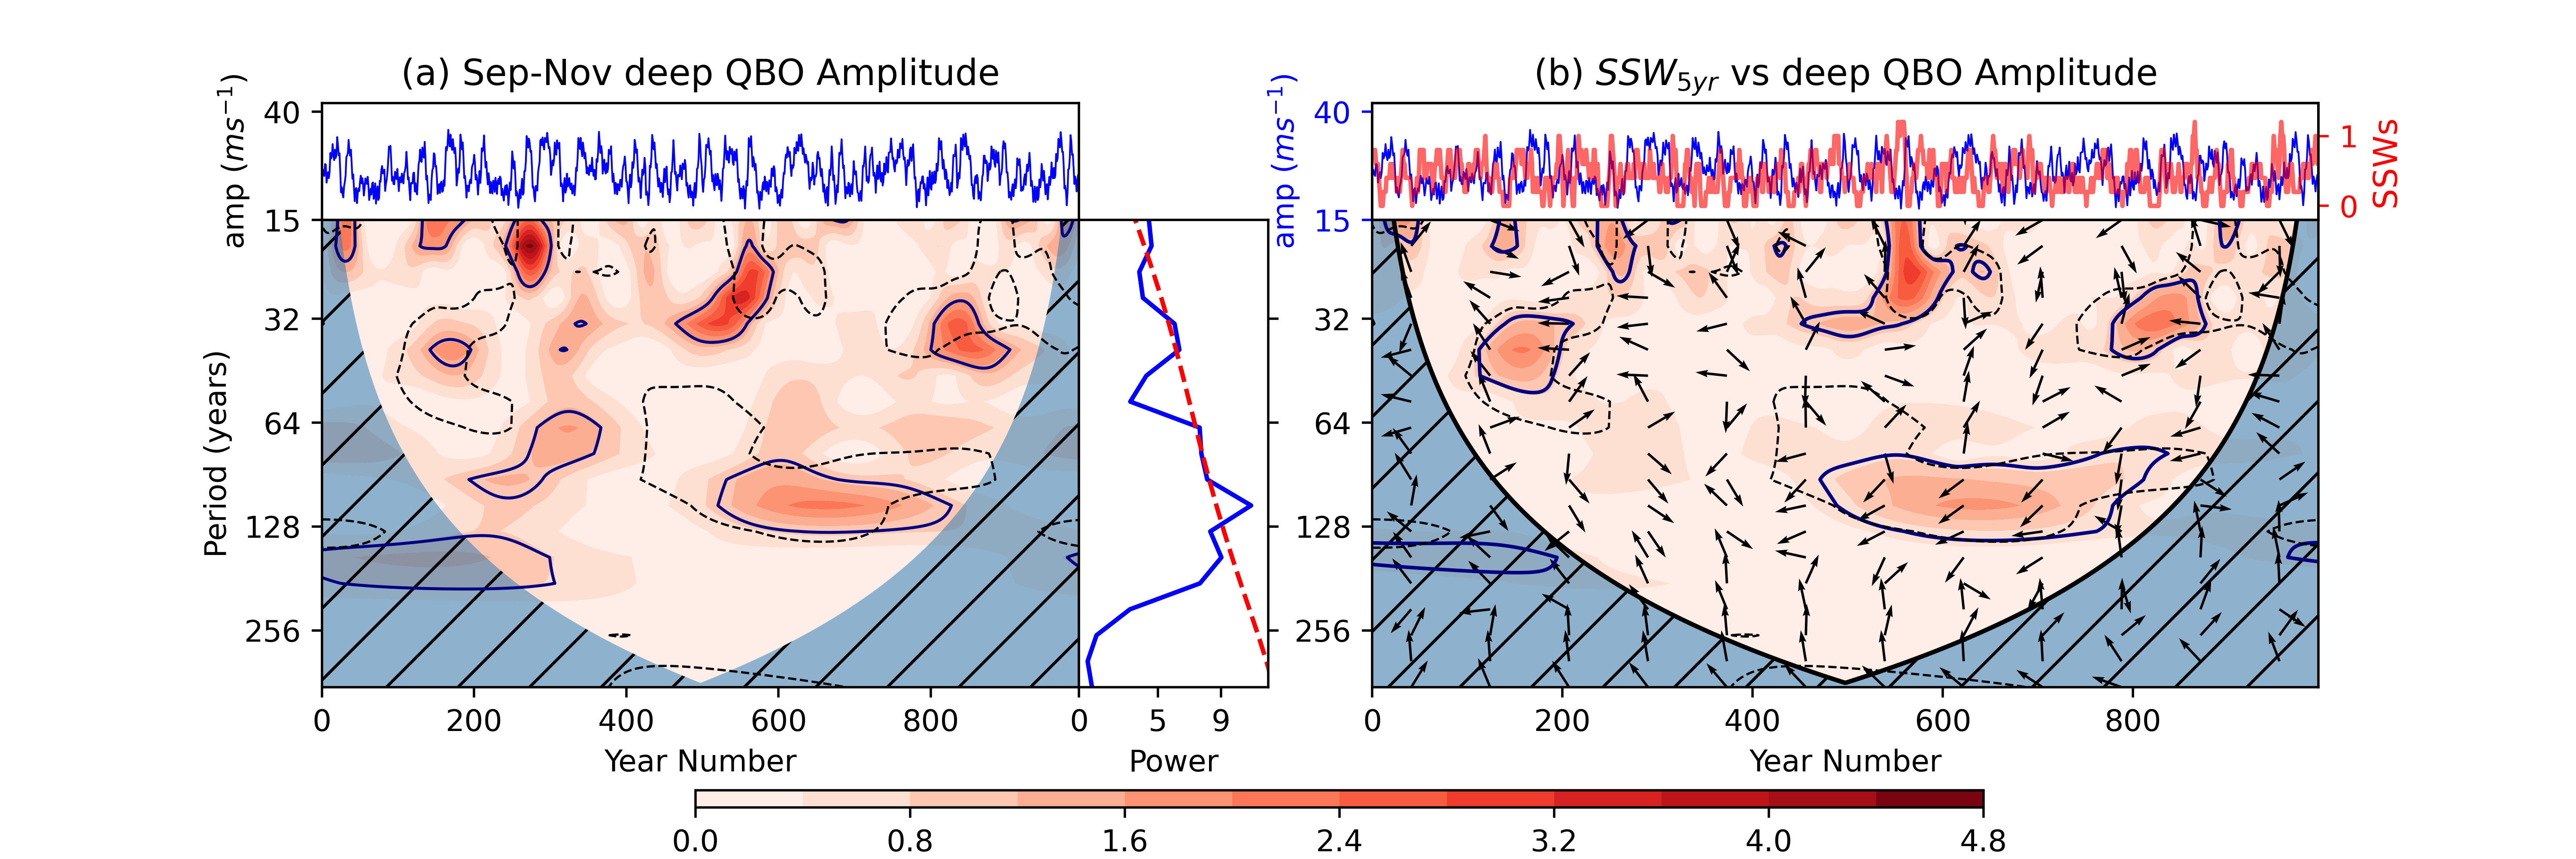
\includegraphics[width = \textwidth]{Figures/Figures-origins/deep_QBO_amp_wavelet_combined.png}
\caption[Wavelet and cross spectra for the deep QBO amplitude in UKESM.]{As figure 8 for the Sep-Nov deep QBO (15--30\,hPa) amplitude index smoothed with a 5 year window. \textbf{a}: QBO amplitude time series and associated wavelet power spectrum, \textbf{b}: Cross power spectrum between deep QBO amplitude and $SSW_5yr$.}
\label{fig:QBO_SSW_subfig}
\end{figure}
\end{center}

%---------------------------------------------------------------


In our earlier discussion we linked long-term variability in SSW frequency to the existence of extended hiatus periods, during which the vortex is relatively undisturbed with no SSW events (figure \ref{fig:SSW_series_sample}). The cross-spectrum analysis with deep QBO amplitude modulation suggests a possible physical interpretation involving the Holton-Tan relationship varying on longer timescales, in which a series of consecutive years that exhibit a large amplitude, deep westerly QBO in early winter leads to a series of winters with reduced SSW frequency i.e. a hiatus period. Correspondingly a series of large-amplitude deep easterly QBO years would lead to a series of consecutive-event years.

We verify the results of the wavelet analyses described above by repeating the multi-linear regression (table 1) but using the 5-year smoothed QBO, ENSO and AL indices to measure their  relative contributions to the 5-year smoothed  $SSW_5yr$ time-series. The resulting regression coefficients for the deep QBO amplitude and AL remain significant at the 95\% level, although the AL's contribution remains small and close to the significance boundary. The coefficient for Ni\~{n}o3.4 is not significant, suggesting that the connection between this ENSO index and the vortex variability is dominated by timescales less than 5 years. If we further isolate multi-decadal signals by fourier filtering each timeseries, so that only periodicities longer than 60 years are retained, the Ni\~{n}o3.4 coefficient is near 0 while the deep QBO amplitude signal is near -0.2. This is consistent with our wavelet analysis which suggest a dominant role for QBO amplitude variations on these long timescales. The AL coefficient remains significant but smaller than that of the QBO (and outside error ranges). For completeness, we repeated the regression analysis using a 5-year smoothed PDO index instead of the AL but there was no significant change in the coefficients (not shown). This is consistent with the fact that the AL and PDO indices exhibit similar spectra and there is a high correlation between them (-0.45 unfiltered and -0.68 filtered), as also found by \cite{mantuaPacific1997a} and \cite{rodionovSpatial2005b}. 

\begin{table}
\centering
\begin{tabular}{|p{3cm}||p{3cm}|p{3cm}|}
 \hline
 \multicolumn{3}{|c|}{SSW$_{5yr}$ regression}\\
 \hline
 Regression Variable& Coefficient& p value\\
 \hline
 Ni\~{n}o3.4  & -0.0127$\pm$0.032& 0.688\\
 AL  &   -0.072$\pm$0.021  & 0.046\\
 deep QBO amp &-0.124$\pm$0.031&0.0001\\
 \hline
\end{tabular}
\begin{center}
\caption{Summary of results from multi-linear regression analysis of SSW$_{5yr}$.} 
\end{center}
\end{table}

\begin{table}
\centering
\begin{tabular}{|p{3cm}||p{3cm}|p{3cm}|}
 \hline
 \multicolumn{3}{|c|}{Filtered (>60 year periods) SSW$_{5yr}$ regression}\\
 \hline
 Regression Variable& Coefficient& p value\\
 \hline
 Ni\~{n}o3.4  &   $\sim$0$\pm$0.01  & $\sim$1\\
 AL & -0.0794$\pm$0.03& 0.042\\
 deep QBO amp &-0.199$\pm$0.01&0.00003\\
 \hline
\end{tabular}
\begin{center}
\caption{Summary of results from multi-linear regression analysis of a fourier filtered version of SSW$_{5yr}$ retaining power corresponding to periods greater than 60 years.}  
\end{center}
\end{table}


To further clarify the role of the QBO, we note that an examination of figure 10 shows that the majority of the long-term amplitude variability in the 15-30 hPa deep QBO index lies in the amplitude of the westerly phase (the easterly phase amplitude is relatively constant with time). Also, as noted earlier, the simulation exhibits more hiatus intervals than consecutive-event intervals, which suggests that the observed long-term variability may arise primarily from the westerly QBO phase. To explore this hypothesis, we isolate the SSW  hiatus intervals by modifying the $SSW_5yr$ time-series in the following way. All SSW rates above 0.54 events per season (the climatological mean) are re-set to 0.54 thereby removing variability in 5 year intervals that exhibit anomalously high SSW rates. Figure \ref{fig:SSW_low_rate_QBO} shows the cross power spectrum between this modified $SSW_5yr$ time-series and the time-series of deep QBO amplitude. It retains significant cross power within the portion of significant $SSW_5yr$ power (figure \ref{fig:SSW_low_rate_QBO} black dashed contours) when compared with figure \ref{fig:QBO_SSW_subfig}b in which the full time-series is used and also shows a phase relationship significantly closer to anti-phased (i.e. pointing to the left). This is further support that the deep QBO - SSW relationship  on these long timescales in the model arises primarily from the SSW hiatus periods. 


\begin{figure}[h!]
\begin{center}
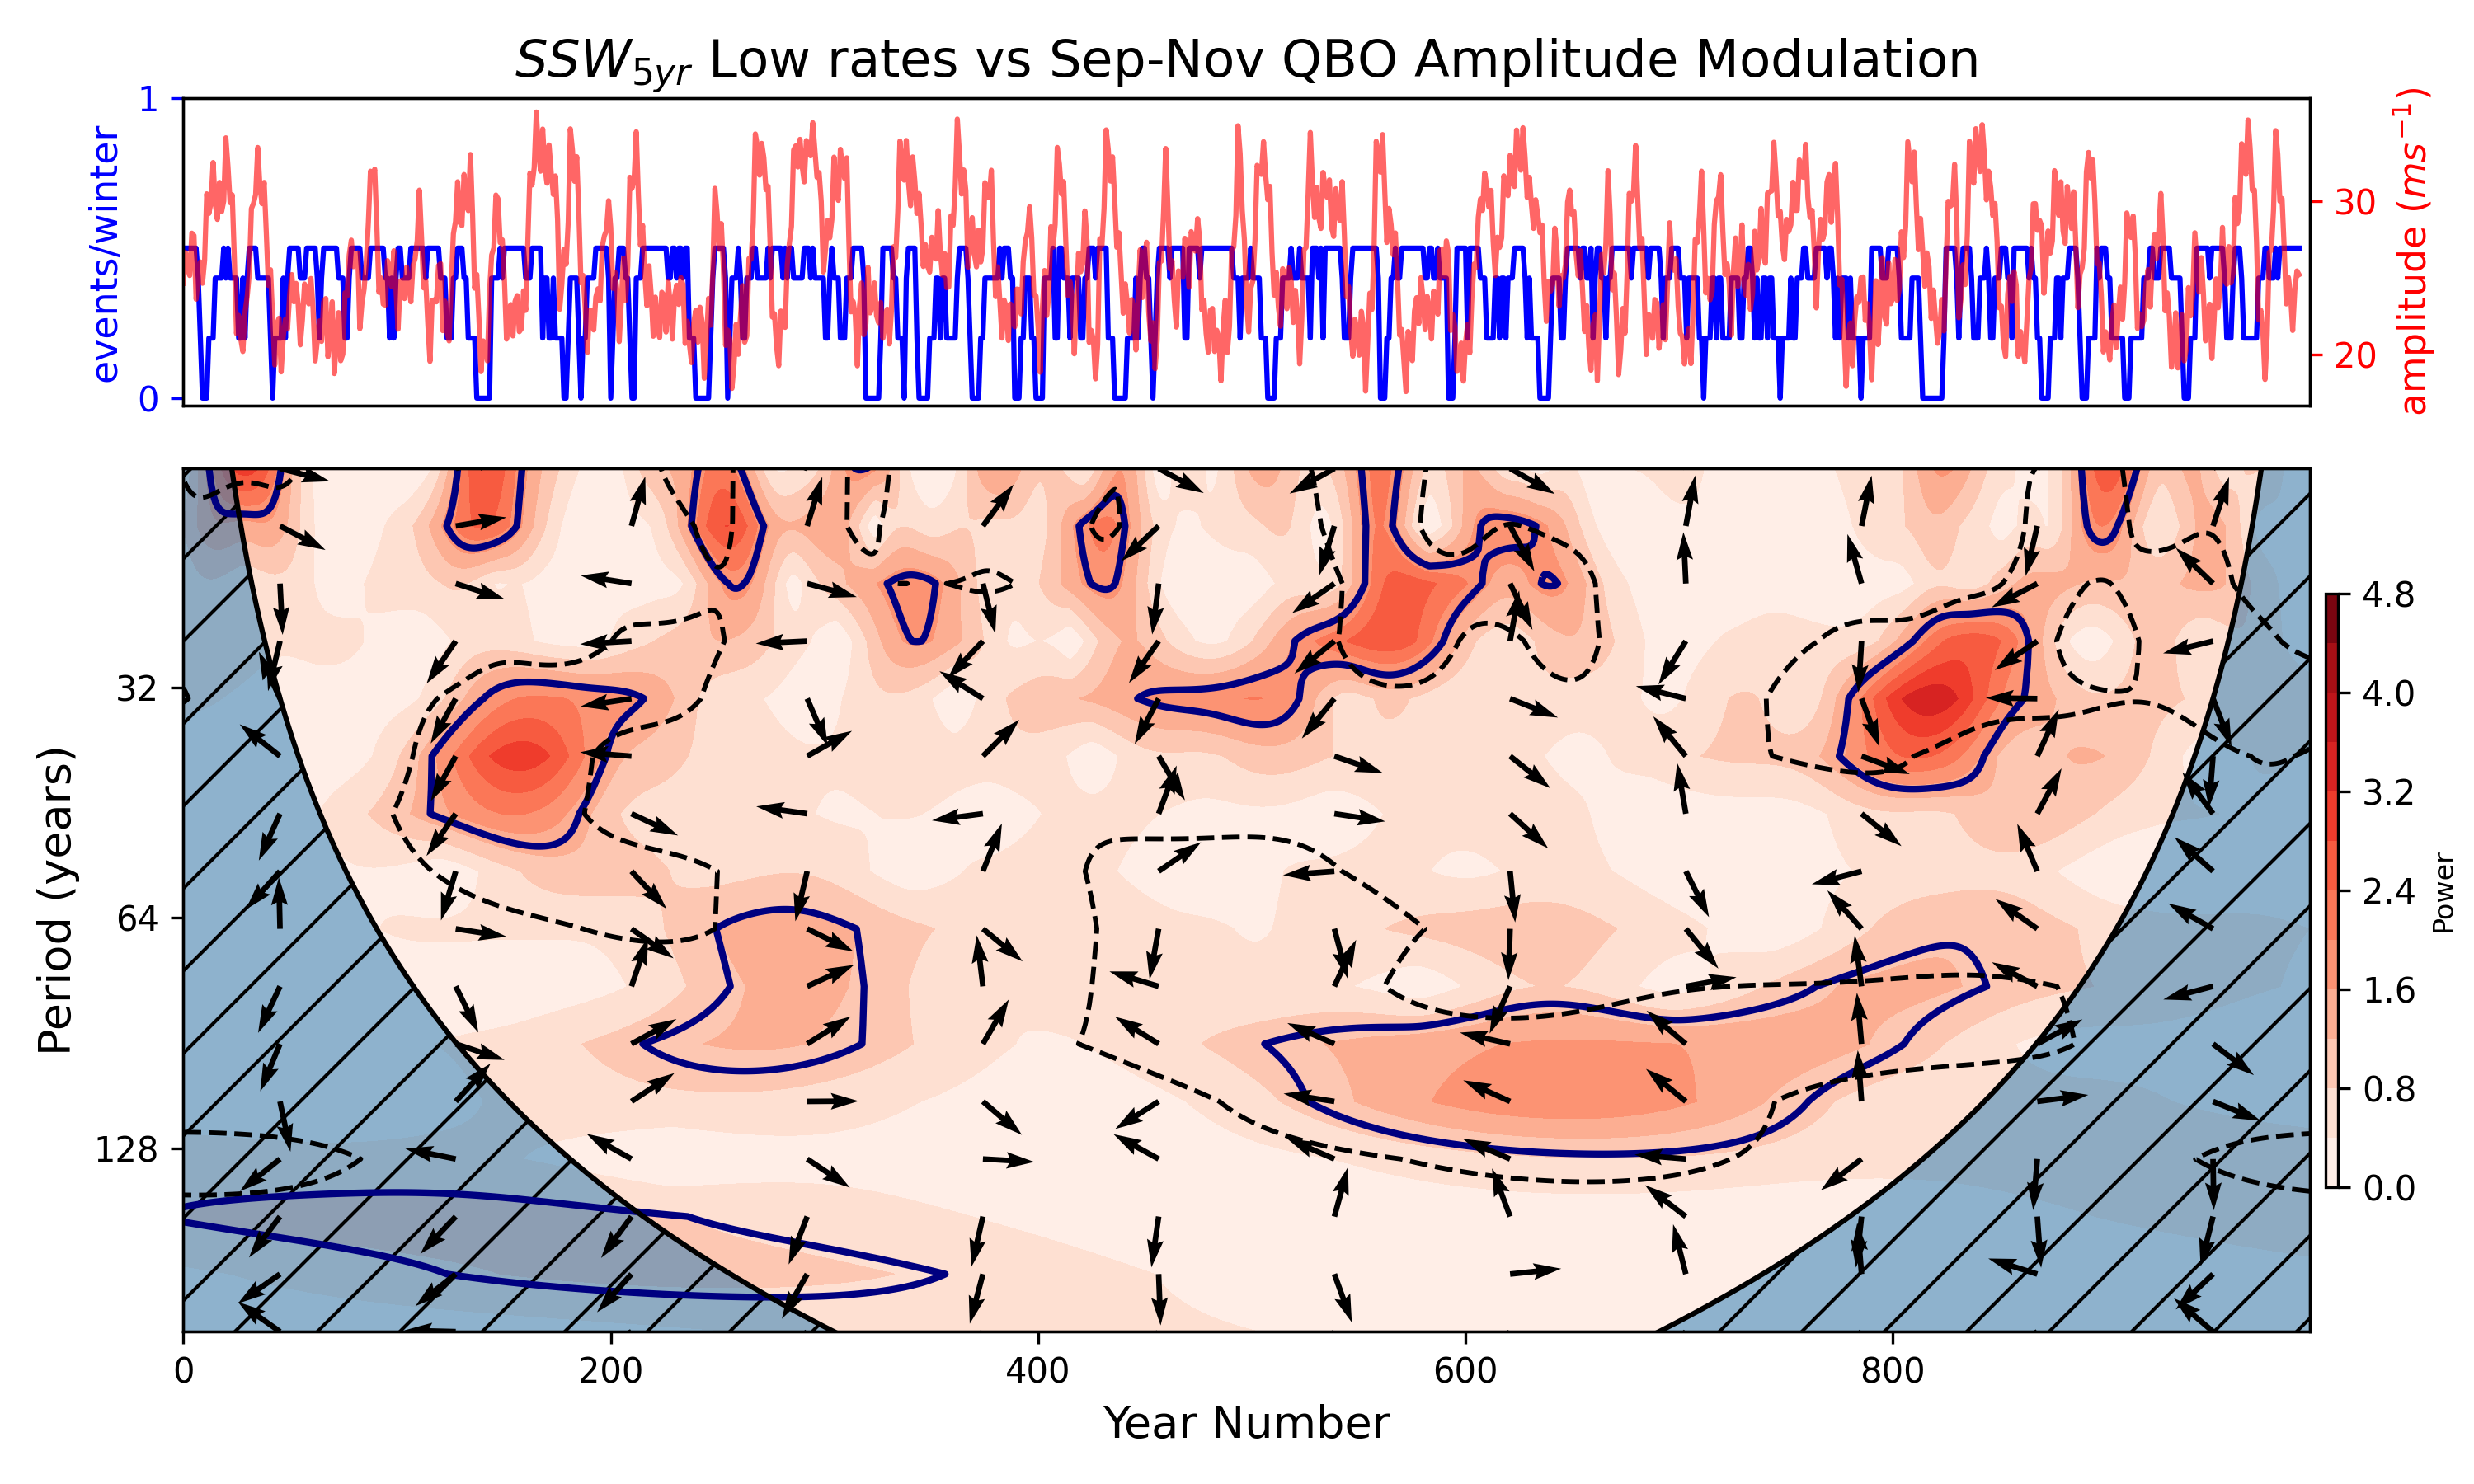
\includegraphics[width = 0.8\linewidth]{Figures/Figures-background/cross_power_SSWs_lowrate_vs_QBO_amplitude_modulation_5yr_mean.png}
\caption[cross power spectrum between deep QBO amplitude and SSW$_{5yr}$ with variations in high SSW rates removed]{\textbf{Top}: $SSW_{5yr}$ time series with variability in high SSW rate intervals removed by setting all rates above the climatological mean (0.54 events per season) to the mean (blue) and Sep-Nov deep QBO Hilbert Amplitude index smoothed with a 5 year window (red). \textbf{Bottom}: Cross wavelet power spectrum between the two time series.}
\label{fig:SSW_low_rate_QBO}
\end{center}
\end{figure}

An obvious question is whether this sensitivity to deep QBO westerlies that we find in the model is also present in the real atmosphere. Examination of the ERA-Interim dataset shows limited support. Some winters in the 1990s are characterised by anomalously westerly Sep-Nov equatorial winds which are vertically coherent between the 15 and 30\,hPa levels. However this effect is intermittent and does not span the whole interval of the 1990s during which SSWs were markedly absent in the observational record (not shown). On the other hand, a mini hiatus that was present in the mid 2010s is associated with 3 years of deep westerly anomaly in the QBO. Overall, it is clear that the relationship, if present in the real atmosphere, is likely obscured by other factors including greenhouse gas increases and volcanic eruptions and the observational dataset is too short to provide useful validation for these long timescale variations.  

\section{Summary and Discussion}
While there is much observational evidence for an impact of SSWs on the underlying tropospheric weather and climate, their multi-decadal variability and the associated forcing mechanisms are not well understood due to the short observational record. Analysis of long climate model simulations is currently the only available tool for understanding this variability. In this chapter we have examined variability in the appearance of hiatus and intervals of consecutive SSWs in a 1000-yr pre-industrial control simulation of one such model (UKESM).

We found realistic decadal and multi-decadal variability in the model, with hiatus intervals of 10 years or more in which no SSWs occurred, similar to the observed SSW record in the 1990s \citep{pawsonCold1999b, Shindell1999} and also intervals of consecutive-event periods in which at least one SSW occurred every year, as observed in the early 2000s \citep{manneyRemarkable2005a}. A 5-yr smoothed representation of SSW frequency ($SSW_{5yr}$) was found to vary periodically for approximately 450 years of the 1000-yr simulation with maxima in wavelet power corresponding to periodicity of around 60-90 years. 

A possible tropical SST source of this long-term variability was investigated. Wavelet and cross-spectrum analyses were performed using a variety of different tropical SST indices, including the ENSO 3.4 index, and also an index of the strength of the Aleutian Low (AL) which is linked to large-scale planetary wave forcing of the winter stratosphere. While all of these indices displayed elements of long-term variability, some of which overlapped with the periodicity and time intervals seen in the $SSW_{5yr}$ spectrum, none of them could fully account for the extended 450 year interval of significant power at 60-90 years seen in the $SSW_{5yr}$ spectrum. The weak relationship between the AL and SSW occurrence is unexpected and modifying the metric by using a box average SLP measure utilised in \cite{garfinkelWhy2012b} did not recover a stronger connection. Further analysis of the AL-SSW relationship in the simulation would be useful to explore whether the AL exhibits a connection with the NH winter mean vortex winds or other continuous vortex metrics such as the NAM even though there is no apparent connection with SSW occurrence. 

A second possible source of long-term variability involving variations in the QBO was also investigated. A range of QBO indices were considered, including the standard approach of using equatorial winds at a specified pressure level e.g. 50 hPa and also a 'deep QBO' index which takes the average QBO wind over 15-30 hPa, designed to capture the degree of vertical coherence in the QBO winds (following \cite{graySurface2018b} and \cite{andrewsObserved2019d}). A straightforward wavelet analysis of these QBO indices reveals no power at periodicity longer than 2-4 years. However, while there is evidently no long-term variability in the frequency of the QBO, visual examination of the QBO time series clearly shows the presence of long-term variability in the QBO amplitudes. A measure of this amplitude modulation was extracted by taking the Hilbert Transform of the QBO index. Wavelet analysis of the amplitude variations from the Hilbert Transform of the QBO indices showed long-term periodicity matching that seen in the $SSW_{5yr}$ wavelet analysis. In particular, the deep QBO index exhibited significant signals coincident with those in $SSW_{5yr}$ corresponding to periodicities of around 90 years. This overlap accounted for nearly all 450 years of SSW variability present on the 90 year timescale. Regression analysis of 5 year smoothed and filtered indices confirmed the contribution of the deep QBO amplitude to variability in SSWs on timescales greater than 60 years. 

Our analysis has therefore revealed an unexpected relationship between the strength and vertical coherence of the QBO and long-term variability in the frequency of SSWs. The relationship was found to be particularly sensitive to the QBO westerly phase. Extended periods of deep westerly QBO phases were associated with hiatus periods with few or no SSWs, consistent with the Holton Tan relationship. While this result appears compelling, it should be noted that the model showed some biases in its QBO associated with the period and descent rate of shear zones. The extended period of close to 3 years could introduce an element of phase locking between the QBO and seasonal cycle causing winter months to occur preferentially in one QBO phase over the other (evident from figure \ref{fig:SSW_hist_QBO_phase}, legends). This may influence QBO-vortex coupling. However, these biases are common in modern GCMs \citep{bushellEvaluation2020b} and \cite{raoModulation2019d} show UKESM's representation of the HT effect is better than most major GCMs submitted to CMIP6 indicating this pi-control remains one of the most effective tools for studying multi-decadal variability in the stratosphere.

Combining the results of all these analyses, our overall conclusion is that multi-decadal variability in SSW frequency in UKESM is primarily accounted for by long term variability in QBO-SSW coupling, particularly at periodicities of around 90 years and, to a lesser extent, by variability in the intensity of the Aleutian Low at periodicities around 60 years, although coherence with the AL signals is far less persistent than with the QBO. Given the observed impact of SSWs on the underlying tropospheric weather and climate, improved understanding of the source and mechanisms of long-term variability in QBO-SSW interactions is likely to help improve future seasonal weather forecasts and decadal-scale climate predictions.

\subsection*{Outlook}
While the results from this chapter provide a novel type of variability in SSWs and its possible origin, the work reveals a number of areas of further research which we aim to address in subsequent chapters of this thesis.

\paragraph{Surface influence of SSW signals:} While we suggest a set of drivers for periodic signals in SSWs, we do not assess the influence of signals in hiatuses on the surface. Of particular interest may be the NH Ocean basins given the timescales of signals considered in this study (similar to characteristic modes of variation such as the AMOC and AMV) as well as vortex variability's association with surface modes in this region \citep{baldwinStratospheric2001a}. Analysis in the following chapter examines the interaction between signals in a vortex timeseries and key modes of tropospheric, surface and Atlantic variability.

\paragraph{Origins of QBO amplitude modulations:} Open questions also remain regarding the role of signals in SSW time series in the earth system. If, as we propose here, amplitude modulation in a deep QBO metric is responsible for driving SSW signals, a natural area of further research could focus on understanding the cause of such amplitude variability. Categorising whether QBO signals are externally driven by features such as tropical upwelling, ENSO (as well as other tropical SST variability) and deep convection or internally generated within the stratosphere would likely be key for this understanding. Work in chapter 4 also includes a closer analysis of tropical upwelling and deep convection in the Pacific region to attempt to diagnose the source of QBO amplitude modulation fully.

\paragraph{The role of QBO vertical structure in teleconnections:} Finally, the precise nature of QBO-SSW interactions is still not fully understood \citep{ansteyHighlatitude2014b}. While the importance of wave-mean flow interactions is widely recognised, further analysis is required to explore the relevance and usefulness of the deep QBO index highlighted in this chapter, that identifies a vertically coherent QBO phase. It appears to be especially relevant to long-term QBO-SSW interactions during the QBO-W phase and its importance is suggested in recent work \citep{andrewsObserved2019d}. Findings from a set of GCM experiments designed to explicitly analyse the role vertical QBO structure in teleconnections are presented in chapter 5. 
